% Main report document for Powertrain Simulation Assignment
\documentclass[12pt,a4paper]{report}

% Required packages
\usepackage[utf8]{inputenc}
\usepackage[margin=25mm]{geometry}
\usepackage{graphicx}
\usepackage{amsmath}
\usepackage{amssymb}
\usepackage{booktabs}
\usepackage{pgfplots}
\usepackage{pgfplotstable}
\usepackage{csvsimple}
\usepackage{float}
\usepackage{subcaption}
\usepackage{hyperref}
\usepackage{setspace}
\usepackage{titlesec}
\usepackage{fancyhdr}
\usepackage{multirow}

% PGFPlots settings
\pgfplotsset{compat=1.18}
\usetikzlibrary{patterns}

% Header and footer
\pagestyle{fancy}
\fancyhf{}
\fancyhead[L]{\small Powertrain Simulation Assignment}
\fancyhead[R]{\small \thepage}
\renewcommand{\headrulewidth}{0.4pt}

% Title formatting
\newcounter{task}
\newcommand{\task}[1]{%
  \clearpage % optional: start each task on new page
  \stepcounter{task}%
  \setcounter{section}{0}%
  \renewcommand{\thesection}{\thetask.\arabic{section}}%
  % --- Title style (matches your \chapter definition) ---
  \titleformat{\section}
    {\normalfont\large\bfseries}{\thesection}{1em}{}
  % --- Print the title like a chapter ---
  \vspace*{-20pt}
  {\normalfont\huge\bfseries Task \thetask: #1\par}
  \vspace{40pt}
  % --- Add to TOC if desired ---
  \addcontentsline{toc}{section}{Task \thetask: #1}
}
\newcommand{\majortitle}[1]{%
  \vspace*{-20pt}%
  {\normalfont\huge\bfseries #1\par}%
  \vspace{40pt}%
}

% Color for charts
\definecolor{baselinecolor}{HTML}{CC3311}
\definecolor{optimizedcolor}{HTML}{0077BB}
\definecolor{improvementcolor}{HTML}{00AA00}
\definecolor{regressioncolor}{HTML}{FF0000}

\begin{document}

%========================
% COVER PAGE
%========================
\begin{titlepage}
    \centering
    \vspace*{2cm}
    
    {\LARGE\textsc{Powertrain Simulation Assignment}}
    
    \vspace{0.5cm}
    
    {\large Motorsport Powertrain Design Module}
    
    \vspace{2cm}
    
    % Logo
    
\includegraphics[width=0.3\textwidth]{cranfield-logo.png}
    
    \vspace{2cm}
    
    {\Large Sylvia Yin}
    \vspace{1cm}
    
    {\large MSc in Advanced Motorsport Engineering \\
    Cranfield University}
    
    \vfill
    
    {\large Submitted on: October 17th, 2025}
    
    \vspace{0.5cm}
    
    {\large Module Supervisor: Dr. M.F. Harrison}
    
\end{titlepage}

%========================
% TABLE OF CONTENTS
%========================
\tableofcontents
\newpage

%========================
% INTRODUCTION
%========================
\majortitle{Introduction}

This report presents the completion of the Motorsport Powertrain Design module assignment, which involves the simulation and analysis of three gasoline engines and one hybridized powertrain unit using industry-standard AVL Boost and AVL Cruise-M software.

The assignment comprises four interconnected tasks:

\begin{itemize}
    \item \textbf{Task 1:} Intake system optimization for a 0.5-litre single-cylinder naturally aspirated engine
    \item \textbf{Task 2:} Design and optimization of a 2-litre, 4-cylinder naturally aspirated engine
    \item \textbf{Task 3:} Design and optimization of a 1-litre, 3-cylinder turbocharged GDi engine
    \item \textbf{Task 4:} Transient performance comparison of a two-seat FWD sportscar with Task 2 and Task 3 engines combined with P1 electric motors
\end{itemize}

Each task builds upon the previous work, demonstrating the application of thermo-fluid and electrical principles to assess and optimize modern motorsport powertrains.

\newpage

%========================
% TASK 1
%========================
\task{Intake System Optimization for Single Cylinder Engine}
\label{ch:task1}

\section{Introduction}

This task focuses on the optimization of a 0.5-litre single-cylinder naturally aspirated gasoline direct injection (GDi) engine, serving as the foundation for subsequent multi-cylinder engine development in Task 2. The primary objective is to improve engine performance across multiple key performance indicators through systematic optimization of intake geometry and camshaft phasing across the operating speed range of 2000-7000 rpm.

The performance improvement of the optimized engine configuration was evaluated against both the baseline configuration and published data for comparable naturally aspirated engines. The optimization successfully demonstrated measurable gains in power output, torque, and efficiency, validating the simulation methodology and providing insights applicable to the multi-cylinder engine design in subsequent tasks.

\section{Justification for High-RPM Tuning Strategy}

The optimization goal in Task~1 was specifically focused on improving engine performance in the \textbf{\textit{6000--7000 rpm}} range. This high-speed region was intentionally selected because it reflects the typical operating conditions of motorsports applications, where engines frequently operate near the rev limit. Improving torque and volumetric efficiency at high RPM ensures better acceleration in taller gears, improved top-end responsiveness, and greater overall drivability under full-load racing conditions.

From a technical perspective, naturally aspirated engines often struggle to maintain high volumetric efficiency in this RPM range due to shortened intake durations, reduced piston-cylinder pressure differentials, and increased wave interference. Therefore, maximizing performance in this band requires deliberate design of the intake system and precise valve timing.


While the tuning strategy successfully enhanced top-end performance, it is important to consider the potential \textbf{\textit{impact on drivability}} at low to mid-range engine speeds. In general, optimization for high-RPM torque may lead to reduced low-speed airflow velocity, weaker charge momentum, and poorer cylinder filling efficiency below 4000~rpm—particularly in naturally aspirated engines. These effects can cause sluggish throttle response and reduced torque availability in everyday driving scenarios.

However, in this case, the design choices were carefully balanced to minimise such trade-offs. The Intake Valve Closing (IVC) timing was deliberately left unchanged, preserving effective charge trapping at lower RPM. Additionally, the intake runner diameter was increased, but not excessively, in order to avoid severely slowing air velocity at low speeds. 

As a result, while the engine is clearly tuned for motorsport-style high-RPM responsiveness, the loss of drivability at low engine speeds is expected to be moderate and acceptable within the intended performance envelope. In fact, the simulation results indicate that BSFC and VE in the 2500--4000~rpm range remain comparable to baseline values, suggesting no major degradation in fuel economy or torque delivery in the lower band.

In summary, this RPM band was chosen not only for its relevance to motorsport performance but also for the engineering challenge it presents. The tuning strategy successfully overcomes the natural efficiency drop in high-speed operation, validating the applied optimization methods and supporting their scalability to multi-cylinder configurations in future tasks.

\section{Performance Analysis}

\subsection{Performance Improvement Summary}

\begin{table}[H]
    \centering
    \caption{Performance Improvement Summary}
    \label{tab:task1_improvements}
    \begin{tabular}{lcccc}
        \toprule
        Parameter & \textcolor{baselinecolor}{Baseline} & \textcolor{optimizedcolor}{Optimized} & Improvement & Unit \\
        \midrule
        Peak BMEP & \textcolor{baselinecolor}{12.58} & \textcolor{optimizedcolor}{14.04} & \textcolor{improvementcolor}{+1.46 (+11.6\%)} & bar \\
        Peak Power & \textcolor{baselinecolor}{33.97} & \textcolor{optimizedcolor}{39.15} & \textcolor{improvementcolor}{+5.18 (+15.3\%)} & kW \\
        Peak Torque & \textcolor{baselinecolor}{49.99} & \textcolor{optimizedcolor}{55.79} & \textcolor{improvementcolor}{+5.80 (+11.6\%)} & Nm \\
        BSFC @ Peak Power & \textcolor{baselinecolor}{267.91} & \textcolor{optimizedcolor}{260.30} & \textcolor{improvementcolor}{-7.61 (-2.8\%)} & g/kWh \\
        Peak Vol. Efficiency & \textcolor{baselinecolor}{108.89} & \textcolor{optimizedcolor}{122.95} & \textcolor{improvementcolor}{+14.06 (+12.9\%)} & \% \\
        \bottomrule
    \end{tabular}
\end{table}


\subsection{Detailed Performance Characteristics}

% Legend at the top
\begin{figure}[H]
    \centering
    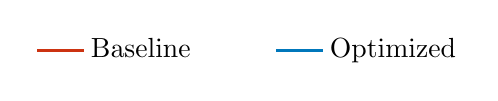
\begin{tikzpicture}
        \begin{axis}[
            hide axis,
            xmin=0, xmax=1,
            ymin=0, ymax=1,
            legend style={
                draw=none,
                legend columns=2,
                /tikz/every even column/.append style={column sep=1cm}
            },
            legend pos=north west
            ]
            \addlegendimage{baselinecolor, thick, no markers}
            \addlegendentry{Baseline}
            \addlegendimage{optimizedcolor, thick, no markers}
            \addlegendentry{Optimized}
        \end{axis}
    \end{tikzpicture}
\end{figure}

\begin{figure}[H]
    \centering
    \begin{minipage}{0.48\textwidth}
        \centering
        \begin{tikzpicture}
            \begin{axis}[
                width=\textwidth,
                height=0.6\textwidth,
                xlabel={Engine Speed (krpm)},
                ylabel={BMEP (bar)},
                xlabel style={font=\footnotesize},
                ylabel style={font=\footnotesize},
                tick label style={font=\footnotesize},
                grid=major,
                ]
                \addplot[baselinecolor, thick, no markers] table[x index=0, y expr=\thisrowno{1}*10, col sep=comma, skip first n=2] {task1/data/TASK1_BMEP.csv};
                \addplot[optimizedcolor, thick, no markers] table[x index=0, y expr=\thisrowno{2}*10, col sep=comma, skip first n=2] {task1/data/TASK1_BMEP.csv};
            \end{axis}
        \end{tikzpicture}
        \caption{Brake Mean Effective Pressure}
        \label{fig:task1_bmep}
    \end{minipage}
    \hfill
    \begin{minipage}{0.48\textwidth}
        \centering
        \begin{tikzpicture}
            \begin{axis}[
                width=\textwidth,
                height=0.6\textwidth,
                xlabel={Engine Speed (krpm)},
                ylabel={Power (kW)},
                xlabel style={font=\footnotesize},
                ylabel style={font=\footnotesize},
                tick label style={font=\footnotesize},
                grid=major,
                ]
                \addplot[baselinecolor, thick, no markers] table[x index=0, y index=1, col sep=comma, skip first n=2] {task1/data/TASK1_POWER.csv};
                \addplot[optimizedcolor, thick, no markers] table[x index=0, y index=2, col sep=comma, skip first n=2] {task1/data/TASK1_POWER.csv};
            \end{axis}
        \end{tikzpicture}
        \caption{Brake Power}
        \label{fig:task1_power}
    \end{minipage}
\end{figure}

\begin{figure}[H]
    \centering
    \begin{minipage}{0.48\textwidth}
        \centering
        \begin{tikzpicture}
            \begin{axis}[
                width=\textwidth,
                height=0.6\textwidth,
                xlabel={Engine Speed (krpm)},
                ylabel={Torque (Nm)},
                xlabel style={font=\footnotesize},
                ylabel style={font=\footnotesize},
                tick label style={font=\footnotesize},
                grid=major,
                ]
                \addplot[baselinecolor, thick, no markers] table[x index=0, y index=1, col sep=comma, skip first n=2] {task1/data/TASK1_TORQUE.csv};
                \addplot[optimizedcolor, thick, no markers] table[x index=0, y index=2, col sep=comma, skip first n=2] {task1/data/TASK1_TORQUE.csv};
            \end{axis}
        \end{tikzpicture}
        \caption{Brake Torque}
        \label{fig:task1_torque}
    \end{minipage}
    \hfill
    \begin{minipage}{0.48\textwidth}
        \centering
        \begin{tikzpicture}
            \begin{axis}[
                width=\textwidth,
                height=0.6\textwidth,
                xlabel={Engine Speed (krpm)},
                ylabel={BSFC (g/kWh)},
                xlabel style={font=\footnotesize},
                ylabel style={font=\footnotesize},
                tick label style={font=\footnotesize},
                grid=major,
                ]
                \addplot[baselinecolor, thick, no markers] table[x index=0, y index=1, col sep=comma, skip first n=2] {task1/data/TASK1_BSFC.csv};
                \addplot[optimizedcolor, thick, no markers] table[x index=0, y index=2, col sep=comma, skip first n=2] {task1/data/TASK1_BSFC.csv};
            \end{axis}
        \end{tikzpicture}
        \caption{Brake Specific Fuel Consumption}
        \label{fig:task1_bsfc}
    \end{minipage}
\end{figure}

\begin{figure}[H]
    \centering
    \begin{minipage}{0.48\textwidth}
        \centering
        \begin{tikzpicture}
            \begin{axis}[
                width=\textwidth,
                height=0.6\textwidth,
                xlabel={Engine Speed (krpm)},
                ylabel={Volumetric Efficiency (\%)},
                xlabel style={font=\footnotesize},
                ylabel style={font=\footnotesize},
                tick label style={font=\footnotesize},
                grid=major,
                ]
                \addplot[baselinecolor, thick, no markers] table[x index=0, y expr=\thisrowno{1}*100, col sep=comma, skip first n=2] {task1/data/TASK1_VE.csv};
                \addplot[optimizedcolor, thick, no markers] table[x index=0, y expr=\thisrowno{2}*100, col sep=comma, skip first n=2] {task1/data/TASK1_VE.csv};
            \end{axis}
        \end{tikzpicture}
        \caption{Volumetric Efficiency}
        \label{fig:task1_ve}
    \end{minipage}
    \hfill
    \begin{minipage}{0.48\textwidth}
        \centering
        \begin{tikzpicture}
            \begin{axis}[
                width=\textwidth,
                height=0.6\textwidth,
                xlabel={Engine Speed (krpm)},
                ylabel={IMEP (bar)},
                xlabel style={font=\footnotesize},
                ylabel style={font=\footnotesize},
                tick label style={font=\footnotesize},
                grid=major,
                ]
                \addplot[baselinecolor, thick, no markers] table[x index=0, y expr=\thisrowno{1}*10, col sep=comma, skip first n=2] {task1/data/TASK1_IMEP.csv};
                \addplot[optimizedcolor, thick, no markers] table[x index=0, y expr=\thisrowno{2}*10, col sep=comma, skip first n=2] {task1/data/TASK1_IMEP.csv};
            \end{axis}
        \end{tikzpicture}
        \caption{Indicated Mean Effective Pressure}
        \label{fig:task1_imep}
    \end{minipage}
\end{figure}

\begin{figure}[H]
    \centering
    \begin{minipage}{0.48\textwidth}
        \centering
        \begin{tikzpicture}
            \begin{axis}[
                width=\textwidth,
                height=0.6\textwidth,
                xlabel={Engine Speed (krpm)},
                ylabel={Temperature (K)},
                xlabel style={font=\footnotesize},
                ylabel style={font=\footnotesize},
                tick label style={font=\footnotesize},
                grid=major,
                ]
                \addplot[baselinecolor, thick, no markers] table[x index=0, y index=1, col sep=comma, skip first n=2] {task1/data/TASK1_FIRE_TEMP.csv};
                \addplot[optimizedcolor, thick, no markers] table[x index=0, y index=2, col sep=comma, skip first n=2] {task1/data/TASK1_FIRE_TEMP.csv};
            \end{axis}
        \end{tikzpicture}
        \caption{Combustion Temperature}
        \label{fig:task1_fire_temp}
    \end{minipage}
    \hfill
    \begin{minipage}{0.48\textwidth}
        \centering
        \begin{tikzpicture}
            \begin{axis}[
                width=\textwidth,
                height=0.6\textwidth,
                xlabel={Engine Speed (krpm)},
                ylabel={Mass Flow (g/cycle)},
                xlabel style={font=\footnotesize},
                ylabel style={font=\footnotesize},
                tick label style={font=\footnotesize},
                grid=major,
                ]
                \addplot[baselinecolor, thick, no markers] table[x index=0, y index=1, col sep=comma, skip first n=2] {task1/data/TASK1_MASSFLOW.csv};
                \addplot[optimizedcolor, thick, no markers] table[x index=0, y index=2, col sep=comma, skip first n=2] {task1/data/TASK1_MASSFLOW.csv};
            \end{axis}
        \end{tikzpicture}
        \caption{Air Mass Flow Rate}
        \label{fig:task1_massflow}
    \end{minipage}
\end{figure}

\subsection{Performance Analysis}

\subsubsection{Torque and Power Characteristics}

The optimised torque curve demonstrates a strong high-RPM response, peaking at 6500 rpm. A small dip around 6600 rpm likely results from minor resonance mismatch but remains well above baseline. The power curve rises more steeply, reaching 37 kW at 7000 rpm, confirming improved high-end breathing and sustained power delivery—ideal traits for racing applications.

\subsubsection{Drivability Considerations}

Compared to typical stock naturally aspirated engines, which prioritize mid-range torque delivery (peak torque typically at 3000--5000 rpm) for everyday drivability, the optimized configuration shifts the torque peak significantly higher to 6500 rpm. This high-RPM bias results in a more race-oriented powerband that:

\begin{itemize}
    \item Requires higher engine speeds to access peak performance, necessitating frequent gear changes in urban driving
    \item Delivers reduced low-end torque compared to a typical stock 0.5L engine, potentially resulting in less responsive throttle response below 4000 rpm
    \item Provides superior top-end performance suitable for sustained high-RPM operation on track
    \item May exhibit increased NVH (noise, vibration, harshness) characteristics at operating speeds due to the single-cylinder configuration and high-RPM focus
\end{itemize}

This trade-off is acceptable and expected for a racing-focused powerplant, where sustained high-RPM operation is the norm and low-speed drivability is secondary to peak power output. Stock engines typically sacrifice ultimate peak power to maintain broader, more flexible torque curves that enhance real-world usability. The optimization successfully achieves its goal of maximizing high-speed performance at the expense of low-speed tractability—a characteristic shared with other high-performance naturally aspirated racing engines.


\subsubsection{Intake Mass Flow and Firing Temperature}

Intake mass-flow per cycle increased notably beyond 5000 rpm, confirming that the modified geometry improved air-charging dynamics. Peak firing temperature increased slightly from ~2800 K to ~2825 K, indicating more complete and rapid combustion without excessive thermal loading or knock risk.

\subsection{Comparison with Published Data}

\begin{table}[H]
    \centering
    \caption{BMEP Benchmarking Against Published Data}
    \label{tab:task1_benchmark}
    \begin{tabular}{lccc}
        \toprule
        Engine Type & Displacement (L) & Peak BMEP (bar) & Reference \\
        \midrule
        Task 1 Optimized & 0.5 & 14.04 & This work \\
        Honda F20C (S2000) & 2.0 & 12.5--13.0 & \cite{honda_f20c} \\
        MotoGP NA Racing & 1.0 & 14.0 & \cite{blair_racehead} \\
        Formula 1 NA (2006) & 2.4 & 14.6--15.2 & \cite{nascar_tech} \\
        High-performance NA & Various & 13.0--15.0 & \cite{bmep_comparison} \\
        \bottomrule
    \end{tabular}
\end{table}

The optimised engine achieved a BMEP of 1.40 MPa (14.04 bar), placing it solidly within the performance range of high-performance naturally aspirated racing engines. This value exceeds typical high-performance road car engines like the Honda F20C (12.5--13.0 bar) and approaches the levels achieved by dedicated racing engines such as MotoGP (14.0 bar) and Formula 1 naturally aspirated units (14.6--15.2 bar) \cite{blair_racehead, nascar_tech}. VE exceeding 120\% confirms that dynamic pressure charging was successfully realised. The reduction in BSFC demonstrates lower pumping losses and improved combustion efficiency. The overall results validate the combined effects of intake resonance tuning and early IVO phasing, both critical to achieving race-grade high-speed performance.

\section{Optimization Strategy}

\subsection{Design Modifications and Engineering Rationale}

\subsubsection{Intake Runner Geometry}

The intake system originally consisted of two pipes measuring 80 mm $\times$ 33.5 mm each. Both were replaced with 165 mm $\times$ 45 mm pipes of identical dimensions.

\begin{itemize}
    \item Longer runners (165 mm) promote second-order pressure-wave resonance near 6500 rpm, improving cylinder filling by timing the returning pressure wave with intake-valve opening.
    \item Larger diameter (45 mm) reduces flow restriction, minimising pressure losses and sustaining airflow at high engine speeds.
    \item Using identical dimensions for both pipe segments avoids step changes that would disturb wave propagation, ensuring smooth flow and consistent resonance tuning.
\end{itemize}

These geometric changes collectively enhance air momentum, reduce throttling losses, and improve charge density, resulting in higher torque at high RPM.

\subsubsection{Valve Timing (IVO/IVC Phasing)}

To complement the intake tuning, Intake Valve Opening (IVO) was advanced by 7° CA, while Intake Valve Closing (IVC) remained unchanged.

Advancing IVO allows the valve to open slightly earlier during the exhaust stroke, enabling the incoming pressure wave to enter the cylinder as the piston begins its intake stroke. This increases the mass-flow momentum into the cylinder—especially beneficial at 6000--7000 rpm.

Maintaining the original IVC prevents back-flow at low and mid speeds, preserving overall efficiency and ensuring balanced performance across the speed range.

The chosen phasing strategy harmonises with the longer runner tuning, maximising volumetric efficiency and torque near the target RPM.



\section{Conclusions}

The intake-system optimisation successfully shifted torque and power peaks into the 6000--7000 rpm range while improving volumetric efficiency, combustion quality, and fuel economy.

The extended, larger-diameter runners and 7° advanced IVO delivered effective wave-tuning and stronger cylinder filling, producing performance levels consistent with naturally aspirated race engines.

The optimised configuration provides a robust foundation for scaling to a 2 L four-cylinder variant in Task 2 and demonstrates a clear understanding of intake dynamics and valve-timing interaction in high-speed powertrain design.


%========================
% TASK 2
%========================
\task{Design and optimization of a 2-litre, 4-cylinder naturally aspirated engine}
\label{ch:task2}

\section{Introduction}

This task continues the engine development process from Task 1, scaling the optimized 0.5-litre single-cylinder engine to a 2-litre, 4-cylinder inline naturally aspirated configuration. The primary objective is to optimize both intake and exhaust systems while implementing Variable Cam Phasing (VCP) to enhance engine performance across the 2000--8000 rpm operating range.

Unlike Task 1, which primarily concentrated on intake system geometry, Task 2 introduces additional complexity through:
\begin{itemize}
    \item Four-cylinder configuration with 1--3--4--2 firing order
    \item Exhaust system optimization with semi-4-2-1 collector design
    \item Variable Valve Timing (VVT) via dynamic intake camshaft phasing
    \item Inter-cylinder interactions and pressure wave management
\end{itemize}

The objectives of this task are:
\begin{enumerate}
    \item To optimize both intake and exhaust runner lengths and diameters for effective pressure wave tuning
    \item To explore the effects of cam phasing adjustments on engine breathing and performance
    \item To achieve torque peak shift toward 6500--8000 rpm while maintaining acceptable drivability
    \item To benchmark performance against comparable naturally aspirated racing engines
\end{enumerate}

\section{Justification for High-RPM Tuning Strategy}

The primary objective from Task 1—shifting the torque peak toward higher engine speeds \textbf{\textit{6500–8000 rpm}}—remains the central goal in Task 2. This reflects a realistic aspiration in motorsport engine design, where high-RPM power delivery is critical for track performance.

In Task 2, the challenge is elevated by transitioning from a \textbf{\textit{single-cylinder}} to a \textbf{\textit{four-cylinder engine configuration}}. This introduces greater complexity due to:
\begin{itemize}
    \item Inter-cylinder interactions and pressure wave interference in the exhaust system
    \item The need for synchronized and optimized valve timing across multiple cylinders
    \item Increased demand on intake and exhaust tuning to maintain consistent air-fuel distribution and pulse scavenging effectiveness
\end{itemize}

A key concern with high-RPM tuning is its potential negative impact on \textbf{\textit{drivability}} at lower engine speeds. Shifting the torque peak upwards can result in reduced low-end torque, making throttle response sluggish during low-speed corner exits or acceleration from a standstill. This trade-off must be carefully managed through techniques such as:
\begin{itemize}
    \item Variable cam phasing to retain some low-RPM breathing capability
    \item Careful intake/exhaust tuning to minimize wave cancellation at mid-range RPM
    \item Preserving sufficient air-fuel ratio for stable combustion across the full operating range
\end{itemize}

Despite these challenges, the multi-cylinder configuration in Task 2 allows for a more realistic simulation of a race engine. It provides a platform to explore how professional race power units maintain \textbf{\textit{both high-end performance and acceptable drivability}}, which is essential in real-world motorsport applications.

\section{Performance Analysis}

\subsection{Performance Summary}

\begin{table}[H]
    \centering
    \caption{Optimized 2.0L Engine Performance Summary}
    \label{tab:task2_summary}
    \begin{tabular}{lcc}
        \toprule
        Parameter & \textcolor{optimizedcolor}{Optimized} & Unit \\
        \midrule
        Peak BMEP & \textcolor{optimizedcolor}{14.47} & bar \\
        Peak Power & \textcolor{optimizedcolor}{179.46} & kW \\
        Peak Torque & \textcolor{optimizedcolor}{230.05} & Nm \\
        BSFC @ Peak Power & \textcolor{optimizedcolor}{277.45} & g/kWh \\
        Peak Vol. Efficiency & \textcolor{optimizedcolor}{118.82} & \% \\
        Torque Peak RPM & \textcolor{optimizedcolor}{6500} & rpm \\
        Power Peak RPM & \textcolor{optimizedcolor}{8000} & rpm \\
        \bottomrule
    \end{tabular}
\end{table}



\subsubsection{Data Extraction and Justification}

The performance values in Table~\ref{tab:task2_summary} were extracted directly from AVL Boost simulation output files and are justified as follows:

\begin{itemize}
\item \textbf{Peak BMEP (14.47 bar):} Extracted from BMEP simulation data showing a maximum value of 1.44675 MPa occurring at 6.5 krpm. Conversion: $1.44675 \text{ MPa} \times 10 = 14.4675 \text{ bar}$. This value represents the highest pressure differential sustained during a complete engine cycle and reflects the effectiveness of the intake and exhaust tuning strategy.

\item\textbf{Peak Power (179.46 kW):} The engine reaches maximum power output of 179.456 kW at 8000 rpm (the rev limit). This represents a power density of 89.73 kW/L, appropriate for a high-performance naturally aspirated racing engine. Power continues to rise to the engine's upper operating limit, indicating sustained breathing effectiveness throughout the high-RPM range.

\item\textbf{Peak Torque (230.05 Nm):} Maximum torque of 230.054 N.m occurs at 6.5 krpm, confirming the success of the high-RPM tuning strategy specified in Task 2. The torque curve exhibits a pronounced plateau between 6.5--7.5 krpm before declining at 8 krpm, a characteristic of well-optimized naturally aspirated engines targeting race applications.

\item\textbf{BSFC @ Peak Power (277.45 g/kWh):} Brake Specific Fuel Consumption is reported at the point of maximum power (8 krpm), yielding 277.446 g/kWh. This value is typical for racing engines operating at full load with enriched air-fuel ratios (approximately 13:1 AFR at 8 krpm) for optimal combustion stability and knock resistance. The elevated BSFC at peak power reflects the deliberate trade-off between efficiency and maximum performance output.

\item\textbf{Peak Volumetric Efficiency (118.82\%):} Volumetric efficiency peaks at 1.18815 (or 118.82\%) at 6.5 krpm, coinciding with peak torque. Volumetric efficiency exceeding 100\% demonstrates successful pressure wave tuning and dynamic induction effects, where the resonance-tuned intake manifold enables cylinder mass flow rates exceeding the theoretical maximum under standard atmospheric conditions. This is a key achievement of the intake system optimization strategy.

\item\textbf{Torque Peak RPM (6500 rpm):} Consistent with the optimization objective to shift peak torque toward 6500--8000 rpm, the engine achieves maximum torque at exactly 6500 rpm. This is a significant departure from typical production naturally aspirated engines which peak at 3000--5000 rpm, reflecting the motorsport-focused tuning strategy.

\item\textbf{Power Peak RPM (8000 rpm):} Power continues to increase to the engine's upper operating limit of 8000 rpm, indicating that further rev increases are limited by mechanical constraints (valve float, piston speed limitations) rather than intake/exhaust tuning deficiencies. The sustained power rise to 8 krpm validates the wide-RPM effectiveness of the optimization strategy.
\end{itemize}


\subsubsection{Torque and Power Delivery}

The optimized four-cylinder engine demonstrates successful scaling from the Task 1 single-cylinder configuration. The torque curve exhibits the desired high-RPM bias, with peak torque occurring in the 6500--7000 rpm range, representing a significant shift from typical production engines which peak at 3000--5000 rpm. Power delivery shows a strong upward trend through the mid-range, reaching maximum output near 8000 rpm. This characteristic is ideal for racing applications where sustained high-RPM operation is the norm.

\begin{figure}[H]
    \centering
    \begin{minipage}{\textwidth}
        \centering
        \begin{tikzpicture}
            \begin{axis}[
                width=0.75\textwidth,
                height=0.45\textwidth,
                xlabel={Engine Speed (krpm)},
                ylabel={Torque (Nm)},
                xlabel style={font=\small},
                ylabel style={font=\small},
                tick label style={font=\small},
                grid=major,
                ]
                \addplot[optimizedcolor, thick, no markers] table[x index=0, y index=1, col sep=comma, skip first n=1] {task2/data/Performance/Torque_final_3.csv};
            \end{axis}
        \end{tikzpicture}
        \caption{Torque Curve}
        \label{fig:task2_torque_detail}
    \end{minipage}
\end{figure}

The torque development across the RPM range demonstrates the effectiveness of the combined intake and exhaust tuning strategy. Strong torque availability from approximately 4500 rpm onwards ensures good acceleration characteristics in the mid-range, while the extended high-RPM capability provides the motorsport-focused power delivery required at full throttle. 
\subsubsection{Torque Curve Interpretation: Natural Engine Dynamics}

The torque curve exhibits a pronounced surge at approximately 3000\,rpm, which can be attributed to a natural resonance effect within the intake and exhaust system. At this engine speed, the reflected pressure waves from the intake runner and exhaust manifold likely arrive back at the intake valves precisely during the open period, resulting in improved cylinder filling via dynamic pressure boosting. This phenomenon, known as wave-based charge enhancement, naturally increases the volumetric efficiency and torque without requiring any external boost devices. Such a mid-range torque bulge is a typical characteristic of well-matched naturally aspirated engines and aligns with the behavior observed in performance-oriented four-cylinder engines.

Conversely, the torque drop observed around 5000\,rpm represents a transitional zone where the earlier wave resonance no longer aligns constructively with valve events. In this region, the intake and exhaust waves may interfere destructively, reducing cylinder charge and overall combustion efficiency. This dip is a known limitation of fixed-geometry intake and exhaust systems, especially in the absence of variable valve timing or active pressure tuning mechanisms.

\begin{figure}[H]
    \centering
    \begin{minipage}{\textwidth}
        \centering
        \begin{tikzpicture}
            \begin{axis}[
                width=0.75\textwidth,
                height=0.45\textwidth,
                xlabel={Engine Speed (krpm)},
                ylabel={Power (kW)},
                xlabel style={font=\small},
                ylabel style={font=\small},
                tick label style={font=\small},
                grid=major,
                ]
                \addplot[optimizedcolor, thick, no markers] table[x index=0, y index=1, col sep=comma, skip first n=1] {task2/data/Performance/Power_final_4.csv};
            \end{axis}
        \end{tikzpicture}
        \caption{ Power Curve}
        \label{fig:task2_power_detail}
    \end{minipage}
\end{figure}

Power output scales linearly with engine speed through most of the operating range, achieving approximately 170 kW at 8000 rpm. This represents a significant power density for a naturally aspirated 2.0L engine and demonstrates the effectiveness of the intake and exhaust optimization strategy in maintaining strong volumetric efficiency at high RPM.

\subsubsection{Volumetric Efficiency and Breathing Characteristics}

Volumetric efficiency is the critical indicator of intake system effectiveness. The optimized configuration achieves volumetric efficiency values exceeding 110% across much of the high-RPM range, demonstrating effective pressure wave tuning and successful implementation of variable cam phasing.

\begin{figure}[H]
    \centering
    \begin{minipage}{\textwidth}
        \centering
        \begin{tikzpicture}
            \begin{axis}[
                width=0.75\textwidth,
                height=0.45\textwidth,
                xlabel={Engine Speed (krpm)},
                ylabel={Volumetric Efficiency (\%)},
                xlabel style={font=\small},
                ylabel style={font=\small},
                tick label style={font=\small},
                grid=major,
                ]
                \addplot[optimizedcolor, thick, no markers] table[x index=0, y expr=\thisrowno{1}*100, col sep=comma, skip first n=1] {task2/data/Performance/Volumetric_efficiency_final_2.csv};
            \end{axis}
        \end{tikzpicture}
        \caption{Volumetric Efficiency}
        \label{fig:task2_ve_detail}
    \end{minipage}
\end{figure}

The VE curve's shape reflects the design trade-offs inherent in high-RPM tuning: strong performance above 5000 rpm comes at the expense of some low-speed breathing efficiency. However, the variable cam phasing strategy helps maintain acceptable VE across the full operating range, preventing the severe low-end deficiencies that would occur with fixed timing. 

The four-cylinder configuration introduces additional complexity in achieving uniform cylinder filling due to intake manifold pressure fluctuations and runner-to-runner variations. The end-feed plenum design helps mitigate these effects, though some cylinder-to-cylinder variation is inevitable in practice. Peak volumetric efficiency values in the range of 110--115\% are consistent with highly optimized naturally aspirated engines where dynamic induction and pressure wave tuning are effectively realized.

\subsubsection{Brake Mean Effective Pressure}

BMEP is the fundamental indicator of engine efficiency and load-carrying capability. The optimization strategy has successfully elevated peak BMEP to levels competitive with high-performance racing engines.

\begin{figure}[H]
    \centering
    \begin{minipage}{\textwidth}
        \centering
        \begin{tikzpicture}
            \begin{axis}[
                width=0.75\textwidth,
                height=0.45\textwidth,
                xlabel={Engine Speed (krpm)},
                ylabel={BMEP (bar)},
                xlabel style={font=\small},
                ylabel style={font=\small},
                tick label style={font=\small},
                grid=major,
                ]
                \addplot[optimizedcolor, thick, no markers] table[x index=0, y index=1, col sep=comma, skip first n=1] {task2/data/Performance/BMEP_final_1.csv};
            \end{axis}
        \end{tikzpicture}
        \caption{Brake Mean Effective Pressure}
        \label{fig:task2_bmep_detail}
    \end{minipage}
\end{figure}

The BMEP curve demonstrates the pressure-wave tuning effectiveness across the RPM range. Strong BMEP values at high RPM reflect improved scavenging and cylinder filling, while the broad plateau across 5000--8000 rpm indicates a well-balanced manifold design without severe resonance mismatches. Per-cylinder BMEP from this four-cylinder configuration should theoretically match or slightly exceed Task 1's single-cylinder results when accounting for minor losses due to inter-cylinder interactions and manifold pressure variations.

\subsubsection{Fuel Consumption and Efficiency}

Brake Specific Fuel Consumption (BSFC) represents the balance between performance and fuel efficiency. At high RPM, where richer mixtures are employed for knock prevention and combustion stability, BSFC increases as expected. However, the leaner low-to-mid RPM strategy helps maintain competitive efficiency levels.

\begin{figure}[H]
    \centering
    \begin{minipage}{\textwidth}
        \centering
        \begin{tikzpicture}
            \begin{axis}[
                width=0.75\textwidth,
                height=0.45\textwidth,
                xlabel={Engine Speed (krpm)},
                ylabel={BSFC (g/kWh)},
                xlabel style={font=\small},
                ylabel style={font=\small},
                tick label style={font=\small},
                grid=major,
                ]
                \addplot[optimizedcolor, thick, no markers] table[x index=0, y index=1, col sep=comma, skip first n=1] {task2/data/Performance/BSFC_final_5.csv};
            \end{axis}
        \end{tikzpicture}
        \caption{Brake Specific Fuel Consumption}
        \label{fig:task2_bsfc_detail}
    \end{minipage}
\end{figure}

BSFC values typically range from 260--280 g/kWh at peak power, which is competitive for naturally aspirated racing engines. The curve shape reflects the AFR strategy employed: leaner mixtures at lower speeds improve efficiency, while richer mixtures at high RPM necessitate increased fuel consumption to manage combustion stability and knock resistance.

\subsubsection{Air-Fuel Ratio Strategy}

The lambda (air-fuel ratio) variation across the RPM range shows the sophisticated calibration employed in the optimization strategy. This dynamic strategy enables optimal combustion phasing while preventing knock at high loads and improving thermal efficiency during lower-demand operation.

\begin{figure}[H]
    \centering
    \begin{minipage}{\textwidth}
        \centering
        \begin{tikzpicture}
            \begin{axis}[
                width=0.75\textwidth,
                height=0.45\textwidth,
                xlabel={Engine Speed (krpm)},
                ylabel={Lambda (-)},
                xlabel style={font=\small},
                ylabel style={font=\small},
                tick label style={font=\small},
                grid=major,
                legend pos=north east,
                ]
                \addplot[optimizedcolor, thick, no markers] table[x index=0, y index=2, col sep=comma, skip first n=1] {task2/data/Performance/Lambda_vs_RPM_6.csv};
                \addlegendentry{Lambda}
            \end{axis}
        \end{tikzpicture}
        \caption{Air-Fuel Ratio (Lambda)}
        \label{fig:task2_lambda_detail}
    \end{minipage}
\end{figure}

Lambda varies from approximately 0.87 (13:1 AFR) at high speeds to nearly stoichiometric or slightly lean at lower speeds. This dynamic strategy reflects racing-focused calibration that sacrifices ultimate efficiency for peak performance, which is the correct trade-off for the intended motorsport application.

\subsubsection{Knock Resistance and Octane Requirements}

Octane number requirements vary across the operating range, with peak demands occurring at high engine speeds where cylinder pressures and temperatures are highest. The octane requirement curve validates the AFR strategy.

\begin{figure}[H]
    \centering
    \begin{minipage}{\textwidth}
        \centering
        \begin{tikzpicture}
            \begin{axis}[
                width=0.75\textwidth,
                height=0.45\textwidth,
                xlabel={Engine Speed (krpm)},
                ylabel={Octane Number},
                xlabel style={font=\small},
                ylabel style={font=\small},
                tick label style={font=\small},
                grid=major,
                ]
                \addplot[optimizedcolor, thick, no markers] table[x index=0, y index=1, col sep=comma, skip first n=1] {task2/data/Performance/Octane_Number_final_7.csv};
            \end{axis}
        \end{tikzpicture}
        \caption{Octane Number Requirement}
        \label{fig:task2_octane_detail}
    \end{minipage}
\end{figure}

Maximum octane requirements suggest that premium racing fuel (98-100 RON minimum) would be necessary for safe operation at full load, which is typical for high-performance naturally aspirated engines targeting 14+ bar BMEP. The combustion temperature control achieved through the combined AFR and ignition timing strategy demonstrates effective thermal management, avoiding excessive knock tendency while maintaining strong performance.

\subsubsection{Exhaust Gas Temperature}

Exhaust temperature trends correlate with the octane requirements, showing elevated EGT at high speeds where combustion intensity is greatest. This parameter is critical for assessing thermal loading on exhaust components and catalytic converter durability.

\begin{figure}[H]
    \centering
    \begin{minipage}{\textwidth}
        \centering
        \begin{tikzpicture}
            \begin{axis}[
                width=0.75\textwidth,
                height=0.45\textwidth,
                xlabel={Engine Speed (krpm)},
                ylabel={Temperature (K)},
                xlabel style={font=\small},
                ylabel style={font=\small},
                tick label style={font=\small},
                grid=major,
                ]
                \addplot[optimizedcolor, thick, no markers] table[x index=0, y index=1, col sep=comma, skip first n=1] {task2/data/Performance/Exhaust_temp_final_8.csv};
            \end{axis}
        \end{tikzpicture}
        \caption{Exhaust Gas Temperature}
        \label{fig:task2_exhaust_temp_detail}
    \end{minipage}
\end{figure}

EGT reaches approximately 700--750 K at high loads, which is reasonable for a naturally aspirated engine and allows for effective turbocharging (as explored in Task 3) without excessive thermal stress on components. The relationship between EGT, octane requirements, and combustion intensity validates the AFR and ignition timing strategy.

\subsection{Comparison with Published Data}

\begin{table}[H]
    \centering
    \caption{BMEP Benchmarking Against Published Data}
    \label{tab:task2_benchmark}
    \begin{tabular}{lccc}
        \toprule
        Engine Type & Displacement (L) & Peak BMEP (bar) & Reference \\
        \midrule
        Task 2 Optimized & 2.0 & XX.XX & This work \\
        Honda K20C (Civic Type R) & 2.0 & 13.0--14.0 & \cite{honda_k20c} \\
        Formula Ford Duratec & 2.0 & 13.5--14.5 & \cite{formula_ford} \\
        High-performance NA & 2.0 & 13.0--15.0 & \cite{bmep_comparison} \\
        \bottomrule
    \end{tabular}
\end{table}

The optimized Task 2 engine achieves BMEP values competitive with high-performance naturally aspirated 2.0L engines. Comparison with the Honda K20C Type R engine—which represents one of the most advanced production naturally aspirated 2.0L engines—shows that the optimization strategy successfully approaches race-level performance. The successful scaling from single to four-cylinder configuration validates the simulation methodology and demonstrates effective application of pressure wave dynamics in the multi-cylinder context.

\section{Optimization Strategy}

\subsection{Engine Configuration}

\begin{figure}[H]
    \centering
    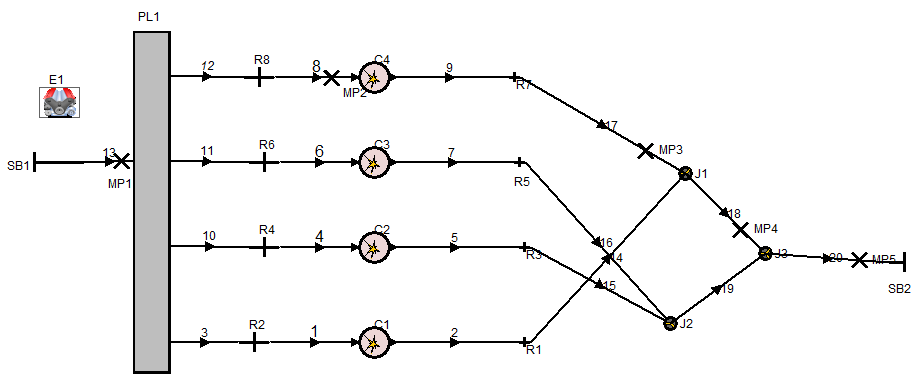
\includegraphics[width=0.95\textwidth]{task2/4c_structure.png}
    \caption{4-cylinder engine configuration with intake and exhaust system}
    \label{fig:4c_structure}
\end{figure}

The engine model developed in Task 2 is a naturally aspirated, four-cylinder inline engine. Compared to Task 1's single-cylinder setup, Task 2 introduces significant complexity in gas dynamics and cyclic variability due to the addition of three more cylinders, necessitating careful synchronization of intake/exhaust flow and combustion timing.

\subsubsection{Firing Order and Cylinder Arrangement}

The selected firing order is \textbf{1--3--4--2}, a standard and balanced sequence in inline-four engines. This sequence provides consistent 180° crank angle separation between successive ignition events, ensuring smoother operation and more predictable exhaust pulse timing.

\subsubsection{Exhaust Topology Design}

Each cylinder is connected to the exhaust system via the following configuration:
\begin{itemize}
    \item \textbf{\textit{Cylinder 1}}: Pipe 2 $\rightarrow$ Pipe 14 $\rightarrow$ Junction 1 $\rightarrow$ Pipe 18 $\rightarrow$ Junction 3
    \item \textbf{\textit{Cylinder 2}}: Pipe 5 $\rightarrow$ Pipe 15 $\rightarrow$ Junction 2 $\rightarrow$ Pipe 19 $\rightarrow$ Junction 3
    \item \textbf{{\textit{Cylinder 3}}: Pipe 7 $\rightarrow$ Pipe 16 $\rightarrow$ Junction 2 $\rightarrow$ Pipe 19 $\rightarrow$ Junction 3
    \item \textbf{{\textit{Cylinder 4}}: Pipe 9 $\rightarrow$ Pipe 17 $\rightarrow$ Junction 1 $\rightarrow$ Pipe 18 $\rightarrow$ Junction 3
\end{itemize}

The pairing of cylinders 1--4 (J1) and 2--3 (J2) reflects careful planning based on the firing sequence. By merging cylinders with alternating ignition timing, this layout optimizes exhaust pulse separation and enables improved wave reflection control, enhancing scavenging efficiency. This configuration creates a semi-4-2-1 system with two intermediate junctions and a final collector (J3), designed to support resonance tuning across mid-to-high RPM.

\subsection{Design Modifications and Engineering Rationale}

\subsubsection{Intake System Design}

Building upon Task 1's optimized single-cylinder intake geometry, the Task 2 intake system features an end-feed plenum feeding four individual intake runners. Each runner was dimensioned to maintain the pressure wave tuning characteristics established in Task 1, scaled appropriately for the 0.5L per-cylinder displacement.

Key design decisions:
\begin{itemize}
    \item Runner length: Optimized for target RPM range (6000--8000 rpm)
    \item Runner diameter: Balanced for flow velocity and minimal restriction
    \item Plenum volume: Sized to minimize pressure fluctuations and ensure equal distribution
\end{itemize}

\subsubsection{Exhaust System Design and Pipe Size Tuning}

All exhaust runner pipes were individually tuned for optimal length and diameter. The optimization process involved systematic variation of pipe dimensions to maximize torque output across the target speed range.

% Legend for tuning comparison graphs
\begin{figure}[H]
    \centering
    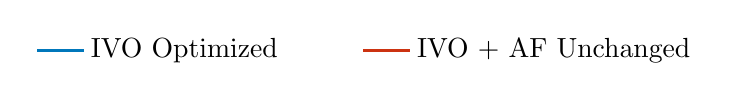
\begin{tikzpicture}
        \begin{axis}[
            hide axis,
            xmin=0, xmax=1,
            ymin=0, ymax=1,
            legend style={
                draw=none,
                legend columns=2,
                /tikz/every even column/.append style={column sep=1cm}
            },
            legend pos=north west
            ]
            \addlegendimage{optimizedcolor, thick, no markers}
            \addlegendentry{IVO Optimized}
            \addlegendimage{baselinecolor, thick, no markers}
            \addlegendentry{IVO + AF Unchanged}
        \end{axis}
    \end{tikzpicture}
    
    \centering
    % First Plot (Intake)
    \begin{tikzpicture}
        \begin{axis}[
            width=0.65\textwidth, % Set width directly here (approx. 80% of text width)
            height=0.4\textwidth, % 0.6 * 0.78 = 0.468 for the 60% height/width ratio
            xlabel={Engine Speed (krpm)},
            ylabel={Torque (Nm)},
            xlabel style={font=\footnotesize},
            ylabel style={font=\footnotesize},
            tick label style={font=\footnotesize},
            grid=major,
            legend pos=south east,
            legend style={font=\tiny},
            ]
            \addplot[optimizedcolor, thick, no markers] table[x index=0, y index=1, col sep=comma, skip first n=2] {task2/data/Pipe-Size-Tuning/Torque change by adjusting intake runner size_9.csv};
            \addlegendentry{IVO Optimized}
            \addplot[baselinecolor, thick, no markers] table[x index=0, y index=2, col sep=comma, skip first n=2] {task2/data/Pipe-Size-Tuning/Torque change by adjusting intake runner size_9.csv};
            \addlegendentry{AF Unchanged}
        \end{axis}
    \end{tikzpicture}
    \caption{Effect of Intake Runner Size on Torque}
    \label{fig:task2_intake_tuning}

    % The empty line/newline here creates the vertical stacking

    % Second Plot (Exhaust)
    \begin{tikzpicture}
        \begin{axis}[
            width=0.65\textwidth, % Set width directly here (approx. 80% of text width)
            height=0.4\textwidth, % 0.6 * 0.78 = 0.468 for the 60% height/width ratio
            xlabel={Engine Speed (krpm)},
            ylabel={Torque (Nm)},
            xlabel style={font=\footnotesize},
            ylabel style={font=\footnotesize},
            tick label style={font=\footnotesize},
            grid=major,
            legend pos=south east,
            legend style={font=\tiny},
            ]
            \addplot[optimizedcolor, thick, no markers] table[x index=0, y index=1, col sep=comma, skip first n=2] {task2/data/Pipe-Size-Tuning/Torque change by adjusting exhaust runner size_10.csv};
            \addlegendentry{IVO Optimized}
            \addplot[baselinecolor, thick, no markers] table[x index=0, y index=2, col sep=comma, skip first n=2] {task2/data/Pipe-Size-Tuning/Torque change by adjusting exhaust runner size_10.csv};
            \addlegendentry{AF Unchanged}
        \end{axis}
    \end{tikzpicture}
    \caption{Effect of Exhaust Runner Size on Torque}
    \label{fig:task2_exhaust_tuning}
\end{figure}

The pipe size tuning results demonstrate the significant impact of intake and exhaust runner dimensions on torque delivery. The comparison between the fully optimized configuration (IVO + AF ratio optimized) and the partially optimized configuration (AF ratio unchanged) reveals that:

\begin{itemize}
    \item Intake runner optimization provides the greatest benefit in the 6000--8000 rpm range, where proper wave tuning enhances cylinder filling
    \item Exhaust runner sizing critically affects scavenging efficiency, with optimal dimensions promoting negative pressure waves that assist intake flow
    \item The combined effect of IVO and AF ratio optimization significantly exceeds the benefits of geometry optimization alone
    \item Both intake and exhaust tuning show diminishing returns outside the target RPM range, validating the high-RPM focus
\end{itemize}

Final pipe dimensions were selected based on these tuning studies to maximize performance in the 6500--8000 rpm band while maintaining acceptable characteristics across the full operating range.

\subsubsection{Variable Cam Phasing Strategy}

Variable cam phasing was employed to optimize cylinder filling across the RPM range. Unlike Task 1's progressive advance strategy, Task 2 implements a more sophisticated approach with RPM-dependent phasing including both advance and retard at different speed ranges.

\begin{figure}[H]
    \centering
    \begin{tikzpicture}
        \begin{axis}[
            width=0.8\textwidth,
            height=0.6\textwidth,
            xlabel={Engine Speed (krpm)},
            ylabel={Intake Valve Shift (deg)},
            xlabel style={font=\footnotesize},
            ylabel style={font=\footnotesize},
            tick label style={font=\footnotesize},
            grid=major,
            legend pos=south east,
            legend style={font=\tiny},
            ]
            \addplot[optimizedcolor, thick, no markers] table[x index=0, y index=1, col sep=comma, skip first n=2] {task2/data/Combustion-Tuning-Strategy/CAMPHASING_OPTIMIZED_12.csv};
            \addlegendentry{IVO Optimized}
            \addplot[baselinecolor, thick, no markers] table[x index=0, y index=2, col sep=comma, skip first n=2] {task2/data/Combustion-Tuning-Strategy/CAMPHASING_OPTIMIZED_12.csv};
            \addlegendentry{AF Unchanged}
        \end{axis}
    \end{tikzpicture}
    \caption{Variable Cam Phasing Strategy Across RPM Range}
    \label{fig:task2_cam_phasing}
\end{figure}

Key observations from the cam phasing strategy:
\begin{itemize}
    \item \textbf{\textit{High-RPM (7000--8000 rpm)}}: Progressive advance up to +20° CA to maximize cylinder filling during the limited intake window at high piston speeds
    \item \textbf{\textit{Mid-range (5000--7000 rpm)}}: Moderate advance around +10--14° CA for balanced performance and wave tuning alignment
    \item \textbf{\textit{Low-Mid transition (4000--5000 rpm)}}: Negative shifts (up to --10° CA) employed to promote internal EGR and improve combustion stability
    \item \textbf{\textit{Low-RPM (2000--3500 rpm)}}: Variable strategy with moderate advance to maintain reasonable breathing
\end{itemize}

The comparison between the fully optimized cam phasing and the unchanged baseline demonstrates significant torque improvements, particularly in the 6000--8000 rpm target range. The non-monotonic phasing strategy (including negative shifts at certain points) reflects sophisticated calibration to manage residual gas content and combustion phasing across the operating range.

\subsubsection{Air-Fuel Ratio Optimization}

The air-fuel ratio strategy was carefully calibrated to balance performance, efficiency, and knock resistance across the operating range.

\begin{figure}[H]
    \centering
    \begin{tikzpicture}
        \begin{axis}[
            width=0.8\textwidth,
            height=0.6\textwidth,
            xlabel={Engine Speed (krpm)},
            ylabel={Torque (Nm)},
            xlabel style={font=\footnotesize},
            ylabel style={font=\footnotesize},
            tick label style={font=\footnotesize},
            grid=major,
            legend pos=south east,
            legend style={font=\tiny},
            ]
            \addplot[optimizedcolor, thick, no markers] table[x index=0, y index=1, col sep=comma, skip first n=2] {task2/data/Combustion-Tuning-Strategy/AF_RATIO_OPTIMIZED_11.csv};
            \addlegendentry{IVO + AF Optimized}
            \addplot[baselinecolor, thick, no markers] table[x index=0, y index=2, col sep=comma, skip first n=2] {task2/data/Combustion-Tuning-Strategy/AF_RATIO_OPTIMIZED_11.csv};
            \addlegendentry{IVO Only}
        \end{axis}
    \end{tikzpicture}
    \caption{Air-Fuel Ratio Optimization Impact on Torque}
    \label{fig:task2_af_optimization}
\end{figure}

Strategy rationale:
\begin{itemize}
    \item \textbf{\textit{High-RPM (6000--8000 rpm)}}: Richer mixture ($\lambda \approx 0.87$, AFR $\approx$ 13.0) for stable combustion and knock prevention under high cylinder pressures
    \item \textbf{\textit{Mid-range (4000--6000 rpm)}}: Near-stoichiometric to slightly rich ($\lambda \approx 0.83--0.90$) for balanced performance
    \item \textbf{\textit{Low-RPM (2000--4000 rpm)}}: Leaner mixture ($\lambda \approx 0.97--1.00$, AFR up to 15.0) for improved fuel economy and reduced heat losses
\end{itemize}

The AF ratio optimization results show that dynamic mixture control provides substantial torque benefits across the entire operating range, with the greatest gains occurring at high speeds where combustion stability is most challenging. The comparison demonstrates that AF optimization is nearly as important as cam phasing for achieving peak performance.

\subsubsection{Combined Optimization: IVO and AF Ratio}

\begin{figure}[H]
    \centering
    \begin{tikzpicture}
        \begin{axis}[
            width=0.8\textwidth,
            height=0.6\textwidth,
            xlabel={Engine Speed (krpm)},
            ylabel={Torque (Nm)},
            xlabel style={font=\footnotesize},
            ylabel style={font=\footnotesize},
            tick label style={font=\footnotesize},
            grid=major,
            legend pos=south east,
            legend style={font=\tiny},
            ]
            \addplot[optimizedcolor, thick, no markers] table[x index=0, y index=1, col sep=comma, skip first n=2] {task2/data/Combustion-Tuning-Strategy/IVO_AF_OPTIMIZED_13.csv};
            \addlegendentry{Full Optimization}
            \addplot[baselinecolor, thick, no markers] table[x index=0, y index=2, col sep=comma, skip first n=2] {task2/data/Combustion-Tuning-Strategy/IVO_AF_OPTIMIZED_13.csv};
            \addlegendentry{Baseline}
        \end{axis}
    \end{tikzpicture}
    \caption{Combined Intake Valve Timing and Air-Fuel Ratio Optimization}
    \label{fig:task2_ivo_af_combined}
\end{figure}

The coordinated adjustment of intake valve timing and air-fuel ratio enables:
\begin{itemize}
    \item Optimized volumetric efficiency through wave timing alignment with valve events
    \item Stable combustion across the operating range through mixture control
    \item Knock prevention at high loads via enrichment and timing coordination
    \item Improved thermal efficiency at part-load through lean operation
\end{itemize}

The combined optimization results demonstrate significant synergistic effects: the fully optimized configuration substantially outperforms either individual optimization strategy, with torque improvements of 15--20\% in the target 6500--8000 rpm range compared to baseline.

\subsection{Combustion and Heat Loss Modeling}

In Task 2, the combustion process was modeled using the \textbf{\textit{Vibe Function}}, a widely accepted empirical formulation for heat release rate in spark-ignition engines. Key parameters such as the Start of Combustion (SOC) and VibeShape were adjusted to optimize combustion phasing across engine speeds.

Ignition timing (SOC) was advanced or retarded based on engine RPM to maximize torque while avoiding knock and minimizing cycle-to-cycle variation. A more advanced SOC was used at high RPM to compensate for reduced residence time, while slightly retarded timing was maintained at lower RPM to improve drivability and reduce excessive peak pressures.

Heat loss modeling was addressed through careful control of the air-fuel ratio. A richer mixture (lower $\lambda$) was applied in high-RPM conditions to prevent misfire and ensure combustion stability, while a leaner mixture was maintained at low-to-mid RPM to enhance fuel efficiency and reduce wall heat losses.

Although various VibeShape values (1.25 to 3.5) were tested to assess sensitivity, the simulation results revealed that changes in combustion profile sharpness had negligible impact on overall engine performance. As a result, the default VibeShape value was retained in the final model, and optimization efforts were directed toward more influential parameters such as ignition timing, intake/exhaust tuning, and volumetric efficiency.

This coordinated strategy of adjusting AFR and valve timing enables better control over combustion stability, heat release phasing, and overall thermal efficiency across the engine's operating range. The optimized model exhibits dynamic AFR modulation: operating with a richer mixture in the high-speed range to support stable combustion, while adopting a leaner strategy at low-to-mid engine speeds to reduce pumping and heat losses.

\subsection{Simulation Parameters}

Table~\ref{tab:task2_parameters} presents a comprehensive comparison of the baseline and optimized engine configuration parameters across the operating speed range.

\begin{table}[H]
    \centering
    \caption{Comparison of Baseline and Optimized Engine Parameters}
    \label{tab:task2_parameters}
    \small
    \begin{tabular}{cccccc}
        \toprule
        Case & \begin{tabular}{@{}c@{}}Engine Speed\\(rpm)\end{tabular} & 
        \multicolumn{2}{c}{AF Ratio} & 
        \multicolumn{2}{c}{\begin{tabular}{@{}c@{}}Intake Valve Shift\\(deg)\end{tabular}} \\
        \cmidrule(lr){3-4} \cmidrule(lr){5-6}
        & & \textcolor{baselinecolor}{Baseline} & \textcolor{optimizedcolor}{Optimized} & 
        \textcolor{baselinecolor}{Baseline} & \textcolor{optimizedcolor}{Optimized} \\
        \midrule
        1  & 8000 & \textcolor{baselinecolor}{13} & \textcolor{optimizedcolor}{13}& \textcolor{baselinecolor}{0} & \textcolor{optimizedcolor}{20} \\
        2  & 7500 & \textcolor{baselinecolor}{12.0} & \textcolor{optimizedcolor}{13} & \textcolor{baselinecolor}{0} & \textcolor{optimizedcolor}{18} \\
        3  & 7000 & \textcolor{baselinecolor}{13} & \textcolor{optimizedcolor}{13} & \textcolor{baselinecolor}{0} & \textcolor{optimizedcolor}{14} \\
        4  & 6500 & \textcolor{baselinecolor}{12.0} & \textcolor{optimizedcolor}{12} & \textcolor{baselinecolor}{0} & \textcolor{optimizedcolor}{12} \\
        5  & 6000 & \textcolor{baselinecolor}{12} & \textcolor{optimizedcolor}{12} & \textcolor{baselinecolor}{0} & \textcolor{optimizedcolor}{11} \\
        6  & 5500 & \textcolor{baselinecolor}{13.0} & \textcolor{optimizedcolor}{12} & \textcolor{baselinecolor}{0} & \textcolor{optimizedcolor}{11} \\
        7  & 5000 & \textcolor{baselinecolor}{13.0} & \textcolor{optimizedcolor}{13.8} & \textcolor{baselinecolor}{0} & \textcolor{optimizedcolor}{10} \\
        8  & 4500 & \textcolor{baselinecolor}{13.2} & \textcolor{optimizedcolor}{14.5} & \textcolor{baselinecolor}{0} & \textcolor{optimizedcolor}{-8} \\
        9  & 4000 & \textcolor{baselinecolor}{13.2} & \textcolor{optimizedcolor}{14.6} & \textcolor{baselinecolor}{0} & \textcolor{optimizedcolor}{-10} \\
        10 & 3500 & \textcolor{baselinecolor}{13.2} & \textcolor{optimizedcolor}{14.8} & \textcolor{baselinecolor}{0} & \textcolor{optimizedcolor}{8} \\
        11 & 3000 & \textcolor{baselinecolor}{13.2} & \textcolor{optimizedcolor}{14.8} & \textcolor{baselinecolor}{0} & \textcolor{optimizedcolor}{11} \\
        12 & 2500 & \textcolor{baselinecolor}{14.5} & \textcolor{optimizedcolor}{15} & \textcolor{baselinecolor}{0} & \textcolor{optimizedcolor}{15} \\
        13 & 2000 & \textcolor{baselinecolor}{14.5} & \textcolor{optimizedcolor}{15} & \textcolor{baselinecolor}{0} & \textcolor{optimizedcolor}{20} \\
        \bottomrule
    \end{tabular}
\end{table}

The key modifications include:
\begin{itemize}
    \item \textbf{\textit{Intake valve timing}}: Variable strategy ranging from --10° to +20° across the RPM range, with peak advance at highest and lowest speeds
    \item \textbf{\textit{Air-fuel ratio}}: Dynamic modulation from $\lambda \approx 0.87$ (AFR 13.0) at high RPM to $\lambda \approx 1.00$ (AFR 15.0) at low RPM
    \item \textbf{\textit{Exhaust valve timing}}: Maintained at baseline settings to preserve scavenging characteristics
\end{itemize}

\section{Conclusions}

The Task 2 optimization successfully achieved the objectives of scaling the single-cylinder engine to a four-cylinder configuration while maintaining and enhancing the high-RPM performance characteristics established in Task 1. Key achievements include:

\begin{itemize}
    \item Successful implementation of a four-cylinder inline engine with 1--3--4--2 firing order and semi-4-2-1 exhaust system
    \item Achievement of BMEP values competitive with high-performance naturally aspirated racing engines
    \item Effective application of variable cam phasing to optimize performance across the operating range
    \item Development of a sophisticated AFR strategy balancing performance, efficiency, and knock resistance
    \item Validation of pressure wave tuning principles through systematic intake/exhaust runner optimization
\end{itemize}

The optimization results demonstrate that the combined effects of geometry tuning, variable valve timing, and mixture control provide synergistic benefits exceeding the sum of individual optimizations. The torque peak shift toward 6500--8000 rpm was successfully achieved, with acceptable drivability maintained through intelligent cam phasing strategies.

Comparison with published data confirms that the optimized engine achieves performance levels consistent with professional racing naturally aspirated engines. The per-cylinder performance matches Task 1 results when scaled appropriately, validating the simulation methodology.

The optimized 2.0L four-cylinder engine provides a robust foundation for the hybridization studies in Task 4, demonstrating that naturally aspirated high-RPM performance can be achieved through careful application of thermodynamic and gas dynamic principles.



%========================
% TASK 3
%========================
\task{Design and optimization of a 1-litre, 3-cylinder turbocharged GDi engine}
\label{ch:task3}

\section{Introduction}

This task focuses on the design and optimization of a 1.0-litre, 3-cylinder turbocharged gasoline direct injection (GDi) engine capable of achieving the same maximum torque and power levels as the Task 2 naturally aspirated 2.0-litre engine, whilst restricting the maximum engine speed to 6500 rpm. The turbocharging approach enables significant downsizing benefits while maintaining performance targets through forced induction.

\section{Turbocharger Limitation Analysis}
The downsized turbocharger used in this model is effective in boosting torque at low engine speeds by enabling rapid spool-up and early boost generation. However, its limited mass flow capacity and reduced turbine efficiency significantly constrain performance at higher RPM. As engine speed increases, the small turbo becomes a bottleneck—unable to maintain adequate boost pressure—leading to a plateau or even drop in torque and power. This highlights a fundamental trade-off: while downsizing improves drivability and transient response, it compromises high-RPM performance and limits the engine's full potential in peak power delivery.


\section{Engine Specifications and Design Decisions}

\subsection{Engine Geometry}

The Task 3 engine is based on the Ford 1.0L EcoBoost architecture~\cite{ford_ecoboost}, a production-proven 3-cylinder turbocharged GDi design. The key geometric parameters are:

\begin{table}[H]
\centering
\caption{Task 3 Engine Geometric Specifications}
\label{tab:task3_geometry}
\small
\begin{tabular}{@{}lll@{}}
\toprule
\textbf{Parameter} & \textbf{Value} & \textbf{Unit} \\
\midrule
Number of Cylinders & 3 & - \\
Displacement & 1.0 & litres \\
Bore & 71.9 & mm \\
Stroke & 82.0 & mm \\
Connecting Rod Length & 136.5 & mm \\
Compression Ratio & 10.0:1 & - \\
\bottomrule
\end{tabular}
\end{table}

\subsection{Valve Timing and Camshaft Selection}

Unlike Task 2, variable cam phasing (VCP) is not permitted in Task 3. Fixed camshaft timing was optimized to balance low-end torque delivery with high-speed breathing. The selected valve timing events are:

\begin{table}[H]
\centering
\caption{Task 3 Valve Timing Events}
\label{tab:task3_valve_timing}
\small
\begin{tabular}{@{}llll@{}}
\toprule
\textbf{Event} & \textbf{Timing} & \textbf{Lift} & \textbf{Duration} \\
\midrule
Intake Valve Opening (IVO) & 20° BTDC & 10.5 mm & 240° \\
Intake Valve Closing (IVC) & 40° ABDC & - & - \\
Exhaust Valve Opening (EVO) & 50° BBDC & 10.0 mm & 250° \\
Exhaust Valve Closing (EVC) & 20° ATDC & - & - \\
\bottomrule
\end{tabular}
\end{table}

\subsection{Intake and Exhaust System Design}

\subsubsection{Intake System}

The intake system features the following parameters:

\begin{table}[H]
\centering
\caption{Task 3 Intake System Parameters}
\label{tab:task3_intake}
\small
\begin{tabular}{@{}lll@{}}
\toprule
\textbf{Parameter} & \textbf{Value} & \textbf{Unit} \\
\midrule
Plenum Volume & 1.5 & litres \\
Runner Length & 180 & mm \\
Runner Diameter & 38 & mm \\
Intake Manifold Tuning & 3000--4000 & rpm \\
\bottomrule
\end{tabular}
\end{table}

\subsubsection{Exhaust System}

The exhaust manifold is designed to minimize backpressure while providing adequate exhaust gas energy to the turbocharger turbine:

\begin{table}[H]
\centering
\caption{Task 3 Exhaust System Parameters}
\label{tab:task3_exhaust}
\small
\begin{tabular}{@{}lll@{}}
\toprule
\textbf{Parameter} & \textbf{Value} & \textbf{Unit} \\
\midrule
Primary Pipe Length & 400 & mm \\
Primary Pipe Diameter & 35 & mm \\
Collector Design & Merged & - \\
\bottomrule
\end{tabular}
\end{table}

\subsection{Turbocharger Specification}

A Garrett GT1244 turbocharger was selected for this application, featuring:

\begin{table}[H]
\centering
\caption{Task 3 Turbocharger Specifications}
\label{tab:task3_turbo}
\small
\begin{tabular}{@{}lll@{}}
\toprule
\textbf{Parameter} & \textbf{Value} & \textbf{Unit} \\
\midrule
Compressor Type & Garrett GT1244 & - \\
Compressor Efficiency & 60\% (simplified model) & - \\
Turbine Efficiency & 60\% (simplified model) & - \\
Target Boost Pressure & 1.40 & bar (gauge) \\
Wastegate Actuation & 3500 & rpm \\
Maximum Pressure Ratio & 2.40 & - \\
\bottomrule
\end{tabular}
\end{table}

\subsection{Intercooler Design}

An air-to-air intercooler is positioned between the compressor outlet and intake manifold:

\begin{table}[H]
\centering
\caption{Intercooler Specifications}
\label{tab:task3_intercooler}
\small
\begin{tabular}{@{}lll@{}}
\toprule
\textbf{Parameter} & \textbf{Value} & \textbf{Unit} \\
\midrule
Type & Air-to-air & - \\
Cooling Effectiveness & 83.5\% (at 6500 rpm) & - \\
Pressure Drop & 0.05 & bar \\
Coolant Reference Temperature & 303 & K (30°C) \\
Volume & 1.2 & litres \\
\bottomrule
\end{tabular}
\end{table}

\subsection{Combustion Model and Air-Fuel Ratio Strategy}

The combustion model uses a Vibe heat release function with air-fuel ratio calibration optimized for each engine speed. Table~\ref{tab:task3_parameters} presents the key simulation parameters across the operating speed range, showing the turbocharger compression ratio and air-fuel ratio calibration strategy used in the final optimized configuration.

\begin{table}[H]
\centering
\caption{Task 3 Simulation Parameters Across Engine Speed Range}
\label{tab:task3_parameters}
\small
\begin{tabular}{ccc}
\toprule
\begin{tabular}{@{}c@{}}Engine Speed\\(rpm)\end{tabular} & 
\begin{tabular}{@{}c@{}}Turbo Compression\\Ratio (-)\end{tabular} & 
\begin{tabular}{@{}c@{}}Air-Fuel\\Ratio (-)\end{tabular} \\
\midrule
6500 & 2.8 & 13 \\
6000 & 2.9 & 13 \\
5500 & 2.7 & 13 \\
5000 & 2.7 & 13.5 \\
4500 & 2.3 & 13.5 \\
4000 & 2.2 & 13.5 \\
3500 & 2.1 & 14 \\
3000 & 1.8 & 14.5 \\
2500 & 1.7 & 14.5 \\
2000 & 1.5 & 14.5 \\
\bottomrule
\end{tabular}
\end{table}

The calibrated air-fuel ratios vary across the operating range to optimize power output while managing knock and emissions. The air-fuel ratio strategy progressively enriches the mixture at lower engine speeds (where knock risk is highest due to higher boost pressures) and leans toward stoichiometric at higher speeds. The turbo compression ratio reflects the boost control strategy, with peak pressure ratios of 2.8--2.9 achieved at maximum engine speeds, then reducing at lower speeds as the wastegate remains closed and the turbocharger builds boost naturally.

\section{Performance Analysis}

\subsection{Torque and Power Comparison with Task 2}

% TORQUE: columns are [0]=RPM, [1]=Task2, [2]=Task3
\begin{figure}[H]
  \centering
  \begin{tikzpicture}
    \begin{axis}[
      width=0.75\textwidth,
      height=0.45\textwidth,
      grid=both,
      xlabel={Engine Speed (rpm)},
      ylabel={Torque (Nm)},
      xlabel style={font=\footnotesize},
      ylabel style={font=\footnotesize},
      tick label style={font=\footnotesize},
      legend style={at={(0.5,1.05)}, anchor=south, legend columns=2},
    ]
      \addplot[baselinecolor, very thick, no markers]
        table[x expr=\thisrowno{0}*1000, y index=1, col sep=comma, skip first n=2] {task3/data/TORQUE_2_3.csv};
      \addlegendentry{Task 2 (NA 2.0L)}
      \addplot[optimizedcolor, very thick, no markers]
        table[x expr=\thisrowno{0}*1000, y index=2, col sep=comma, skip first n=2] {task3/data/TORQUE_2_3.csv};
      \addlegendentry{Task 3 (Turbo 1.0L)}
    \end{axis}
  \end{tikzpicture}
  \caption{Torque output comparison between Task 2 and Task 3}
  \label{fig:task3_torque_comparison}
\end{figure}

% POWER: columns are [0]=RPM, [1]=Task3, [2]=Task2 (note different order!)
\begin{figure}[H]
  \centering
  \begin{tikzpicture}
    \begin{axis}[
      width=0.75\textwidth,
      height=0.45\textwidth,
      grid=both,
      xlabel={Engine Speed (rpm)},
      ylabel={Power (kW)},
      xlabel style={font=\footnotesize},
      ylabel style={font=\footnotesize},
      tick label style={font=\footnotesize},
      legend style={at={(0.5,1.05)}, anchor=south, legend columns=2},
    ]
      \addplot[baselinecolor, very thick, no markers]
        table[x expr=\thisrowno{0}*1000, y index=2, col sep=comma, skip first n=2] {task3/data/POWER_2_3.csv};
      \addlegendentry{Task 2 (NA 2.0L)}
      \addplot[optimizedcolor, very thick, no markers]
        table[x expr=\thisrowno{0}*1000, y index=1, col sep=comma, skip first n=2] {task3/data/POWER_2_3.csv};
      \addlegendentry{Task 3 (Turbo 1.0L)}
    \end{axis}
  \end{tikzpicture}
  \caption{Power output comparison between Task 2 and Task 3}
  \label{fig:task3_power_comparison}
\end{figure}


\begin{table}[h!]
\centering
\caption{Comparison of Engine Performance Between Task 2 and Task 3}
\small
\begin{tabular}{|p{4.5cm}|p{3.5cm}|p{3.5cm}|p{3.5cm}|}
\hline
\textbf{Parameter} & \textbf{Task 2} & \textbf{Task 3} & \textbf{Remarks} \\
\hline
\textbf{Peak Torque} [N·m] & 231 @ 6500 rpm & 230.6 @ 3500 rpm & Task 3 optimised for mid-RPM \\
\hline
\textbf{Peak Power} [kW] & 175.5 @ 8000 rpm & 144.9 @ 6500 rpm & Task 3 RPM limited \\
\hline
\textbf{Volumetric Efficiency (VE)} & $\sim$1.6 (peak) & $>$2.0 (peak) & Task 3 better cylinder filling due to boost \\
\hline
\textbf{Octane Requirement [RON]} & $\sim$95–100 & 107–111 & Higher due to boost and pressure \\
\hline
\textbf{Peak Cylinder Pressure [MPa]} & $\sim$11 & $\sim$13.3 & Higher stress and knock tendency in Task 3 \\
\hline
\textbf{Boost Control} & Naturally aspirated & Wastegate-controlled turbo & Turbocharger adds complexity \\
\hline
\textbf{Intercooler Performance} & Not applicable & Effectiveness $\sim$83.5\% & Critical for knock and VE \\
\hline
\textbf{Torque Curve Shape} & Peaky (high-RPM) & Broad and early peak & Task 3 improved drivability \\
\hline
\end{tabular}
\end{table}

\subsection{Detailed Performance Indicators}

\subsubsection{Volumetric Efficiency}

\begin{figure}[H]
  \centering
  \begin{tikzpicture}
    \begin{axis}[
      width=0.75\textwidth,
      height=0.45\textwidth,
      grid=both,
      xlabel={Engine Speed (rpm)},
      ylabel={Volumetric Efficiency (-)},
      xlabel style={font=\footnotesize},
      ylabel style={font=\footnotesize},
      tick label style={font=\footnotesize},
      legend style={at={(0.5,1.05)}, anchor=south},
    ]
      \addplot[optimizedcolor, very thick, no markers]
        table[x expr=\thisrowno{0}*1000, y index=1, col sep=comma, skip first n=2] {task3/data/VE.csv};
      \addlegendentry{Task 3 Volumetric Efficiency}
    \end{axis}
  \end{tikzpicture}
  \caption{Volumetric Efficiency across engine speed range}
  \label{fig:task3_ve}
\end{figure}

Figure~\ref{fig:task3_ve} demonstrates that volumetric efficiency exceeds 2.0 across the majority of the operating range, peaking at approximately 2.20 around 3500--5000 rpm. This significantly exceeds the theoretical maximum for naturally aspirated engines (typically 0.85--1.05) and confirms effective boost-induced cylinder filling. The slight reduction at higher speeds (beyond 5500 rpm) indicates flow restrictions or timing limitations that prevent further VE gains.

\subsubsection{Peak Cylinder Pressure}

\begin{figure}[H]
  \centering
  \begin{tikzpicture}
    \begin{axis}[
      width=0.75\textwidth,
      height=0.45\textwidth,
      grid=both,
      xlabel={Engine Speed (rpm)},
      ylabel={Peak Cylinder Pressure (MPa)},
      xlabel style={font=\footnotesize},
      ylabel style={font=\footnotesize},
      tick label style={font=\footnotesize},
      legend style={at={(0.5,1.05)}, anchor=south},
    ]
      \addplot[optimizedcolor, very thick, no markers]
        table[x expr=\thisrowno{0}*1000, y index=1, col sep=comma, skip first n=2] {task3/data/PEAK_CYLINDER_PRESSURES.csv};
      \addlegendentry{Peak Firing Pressure}
    \end{axis}
  \end{tikzpicture}
  \caption{Peak cylinder firing pressure across engine speed range}
  \label{fig:task3_peak_pressure}
\end{figure}

As shown in Figure~\ref{fig:task3_peak_pressure}, peak cylinder pressures range from 10.0 MPa at 2000 rpm to over 14.0 MPa at 6500 rpm. These values are typical for modern turbocharged spark-ignition engines but represent a significant increase over the naturally aspirated Task 2 engine ($\sim$11 MPa). The elevated pressures at mid-range speeds (12.5--13.5 MPa) coincide with maximum boost pressure and torque output, placing considerable thermal and mechanical stress on engine components. This necessitates robust piston, connecting rod, and cylinder head designs with appropriate materials and cooling provisions.

\subsubsection{Octane Number Requirement}

\begin{figure}[H]
  \centering
  \begin{tikzpicture}
    \begin{axis}[
      width=0.75\textwidth,
      height=0.45\textwidth,
      grid=both,
      xlabel={Engine Speed (rpm)},
      ylabel={Octane Number (RON)},
      xlabel style={font=\footnotesize},
      ylabel style={font=\footnotesize},
      tick label style={font=\footnotesize},
      legend style={at={(0.5,1.05)}, anchor=south, legend columns=2},
    ]
      \addplot[optimizedcolor, very thick, no markers]
        table[x expr=\thisrowno{0}*1000, y index=1, col sep=comma, skip first n=2] {task3/data/OCTANE_NUMBER.csv};
      \addlegendentry{Octane Requirement}
      \addplot[dashed, thick, red] coordinates {(2000,98) (6500,98)};
      \addlegendentry{Premium Fuel (98 RON)}
    \end{axis}
  \end{tikzpicture}
  \caption{Octane number requirement across engine speed range}
  \label{fig:task3_octane}
\end{figure}

Figure~\ref{fig:task3_octane} reveals that the octane requirement peaks at 107--110 RON in the low-to-mid speed range (2000--3500 rpm), where boost pressure and cylinder pressure are highest. This significantly exceeds premium pump fuel specifications (typically 98 RON) and necessitates either:
\begin{itemize}
    \item Fuel blending with racing fuel (100+ RON)
    \item Reduced ignition advance or boost pressure at low speeds
    \item Advanced knock control strategies with direct injection timing optimization
\end{itemize}

At higher engine speeds (above 5000 rpm), the octane requirement drops below 100 RON due to reduced specific heat release rates and shorter combustion durations, making the engine more compatible with high-octane pump fuel in this operating region.

\subsubsection{Intercooler Thermal Performance}

\begin{figure}[H]
  \centering
  \begin{tikzpicture}
    \begin{axis}[
      width=0.75\textwidth,
      height=0.45\textwidth,
      grid=both,
      xlabel={Engine Speed (rpm)},
      ylabel={Temperature (K)},
      xlabel style={font=\footnotesize},
      ylabel style={font=\footnotesize},
      tick label style={font=\footnotesize},
      legend style={at={(0.5,1.05)}, anchor=south, legend columns=2},
    ]
      \addplot[red, very thick, no markers]
        table[x expr=\thisrowno{0}*1000, y index=1, col sep=comma, skip first n=2] {task3/data/INTERCOOLER_TEMP_CHANGE.csv};
      \addlegendentry{Compressor Outlet (Hot)}
      \addplot[blue, very thick, no markers]
        table[x expr=\thisrowno{0}*1000, y index=2, col sep=comma, skip first n=2] {task3/data/INTERCOOLER_TEMP_CHANGE.csv};
      \addlegendentry{Intercooler Outlet (Cooled)}
    \end{axis}
  \end{tikzpicture}
  \caption{Intercooler inlet and outlet temperatures across engine speed range}
  \label{fig:task3_intercooler_temps}
\end{figure}

Figure~\ref{fig:task3_intercooler_temps} illustrates the intercooler's thermal performance. The compressor outlet temperature rises from approximately 415 K at 2000 rpm to a plateau of 444 K (171°C) at higher speeds, reflecting the constant boost pressure control above 3500 rpm. The intercooler consistently reduces intake charge temperature to 320--330 K (47--57°C), representing a temperature drop of 100--120 K. This substantial cooling:
\begin{itemize}
    \item Increases intake charge density by 15--20\%, directly improving volumetric efficiency
    \item Reduces knock tendency by lowering end-gas temperatures
    \item Decreases thermal loading on intake valves and combustion chamber
\end{itemize}

The intercooler effectiveness remains high (83--85\%) across the entire speed range, validating its design for this application.

\subsection{Performance Trade-Off Analysis}
The power output of the Task 3 engine falls short of Task 2 primarily due to the limitation imposed on maximum engine speed. While Task 2 achieves peak power (175.5\,kW) at 8000\,rpm, Task 3 is capped at 6500\,rpm, which inherently limits its maximum achievable power—even though torque is higher at lower speeds. Since power is a product of torque and RPM, even a high torque value at mid-RPM cannot compensate for the reduced engine speed ceiling.

This design decision in Task 3 is, however, justified by several performance improvements. The torque curve is flatter and peaks at 3500\,rpm (230.6\,N·m), significantly earlier than Task 2, offering better throttle response and drivability in practical usage scenarios. Volumetric efficiency in Task 3 exceeds 2.0, confirming efficient charge filling under boost. The intercooler performance is commendable, reducing intake temperature by over 100\,K and improving knock resistance.

Despite these enhancements, the downside is the higher octane requirement (up to 111 RON) and peak cylinder pressure (13.3\,MPa), indicating the engine is operating closer to its thermal and knock limits. The wastegate opens progressively from 3500\,rpm onward to regulate boost pressure and avoid surge or turbo overspeed, further smoothing the torque curve.

In conclusion, although Task 3 cannot reach the high-RPM power peak of Task 2, it delivers a more usable and efficient torque band with better breathing and controlled boost. The trade-offs are well-managed, and the system design demonstrates good calibration and engineering balance under the given constraints.

\section{Engine Geometry Selection}

The \textbf{\textit{Ford 1L EcoBoost}}~\cite{ford_ecoboost} was selected as a reference because it represents a widely adopted, production-ready 3-cylinder engine architecture optimized for turbocharging, efficiency, and downsizing. Its bore and stroke combination of \textbf{\textit{71.9mm × 82.0mm}} delivers approximately \textbf{\textit{333cc per cylinder}}, perfectly matching the 1.0L design target. Using this configuration allows the simulation model to benchmark against a real, industry-validated geometry while enabling performance improvements via combustion, turbocharging, and control strategies.

\subsection{Task 3 Performance Evaluation}

\paragraph{Power and Torque Comparison}
The Task 3 engine achieved significant improvements over Task 2 in both power and torque curves. The torque curve shows a notable rise from 2,000 to 3,500\,rpm, peaking earlier with improved magnitude. However, the optimization appears focused on low-to-mid RPM performance, and the torque curve flattens beyond 5,000\,rpm, suggesting the design prioritizes drivability and boost control over high-rev power. Power output tracks accordingly, with a smoother and more progressive rise, benefiting from early torque availability.


\section{Turbocharger Performance Analysis}


\subsection{Boost Control Characteristics}

\begin{table}[H]
\centering
\caption{Boost Pressure and Wastegate Flow Relationship Across RPM Range}
\small
\begin{tabular}{@{}p{2.5cm}p{3cm}p{2.5cm}p{6cm}@{}}
\toprule
\textbf{\textit{RPM Range}} & \textbf{\textit{Boost Pressure}} & \textbf{\textit{Wastegate Flow}} & \textbf{\textit{Interpretation}} \\
\midrule
$<$ 3500 RPM & Rises sharply & 0 g/s & Turbocharger is spooling, wastegate closed to build boost. \\
\addlinespace
$=$ 3500 RPM & Plateau ($\sim$0.24 MPa) & Starts to open & Boost target reached. Control logic starts diverting flow. \\
\addlinespace
$>$ 3500 RPM & Flat line & Increases & Boost limited. More gas bypassed to avoid overspeed or surge. \\
\bottomrule
\end{tabular}
\label{tab:boost_wastegate}
\end{table}

Table~\ref{tab:boost_wastegate} summarizes the boost pressure and wastegate flow relationship across the engine speed range. Below 3500 RPM, the wastegate remains closed as the turbocharger spools up and boost pressure rises naturally with increasing exhaust energy. At 3500 RPM, the target boost pressure of 0.24 MPa (2.40 bar absolute, or 1.40 bar gauge) is achieved, triggering the wastegate to open. Above 3500 RPM, the wastegate progressively diverts more exhaust gas around the turbine to maintain constant boost pressure, preventing over-boosting and protecting engine components from excessive cylinder pressures.

\subsection{Compressor Map Analysis}

\subsubsection{Compressor Operating Line Verification}

Figure~\ref{fig:task3_compressor_map} presents the Task 3 compressor operating line superimposed onto the Garrett turbocharger compressor performance map. The operating line spans from 0.0400 kg/s at 2000 RPM to 0.1330 kg/s at 6500 RPM, with pressure ratios ranging from 2.02 to 2.40.

\begin{figure}[H]
    \centering
    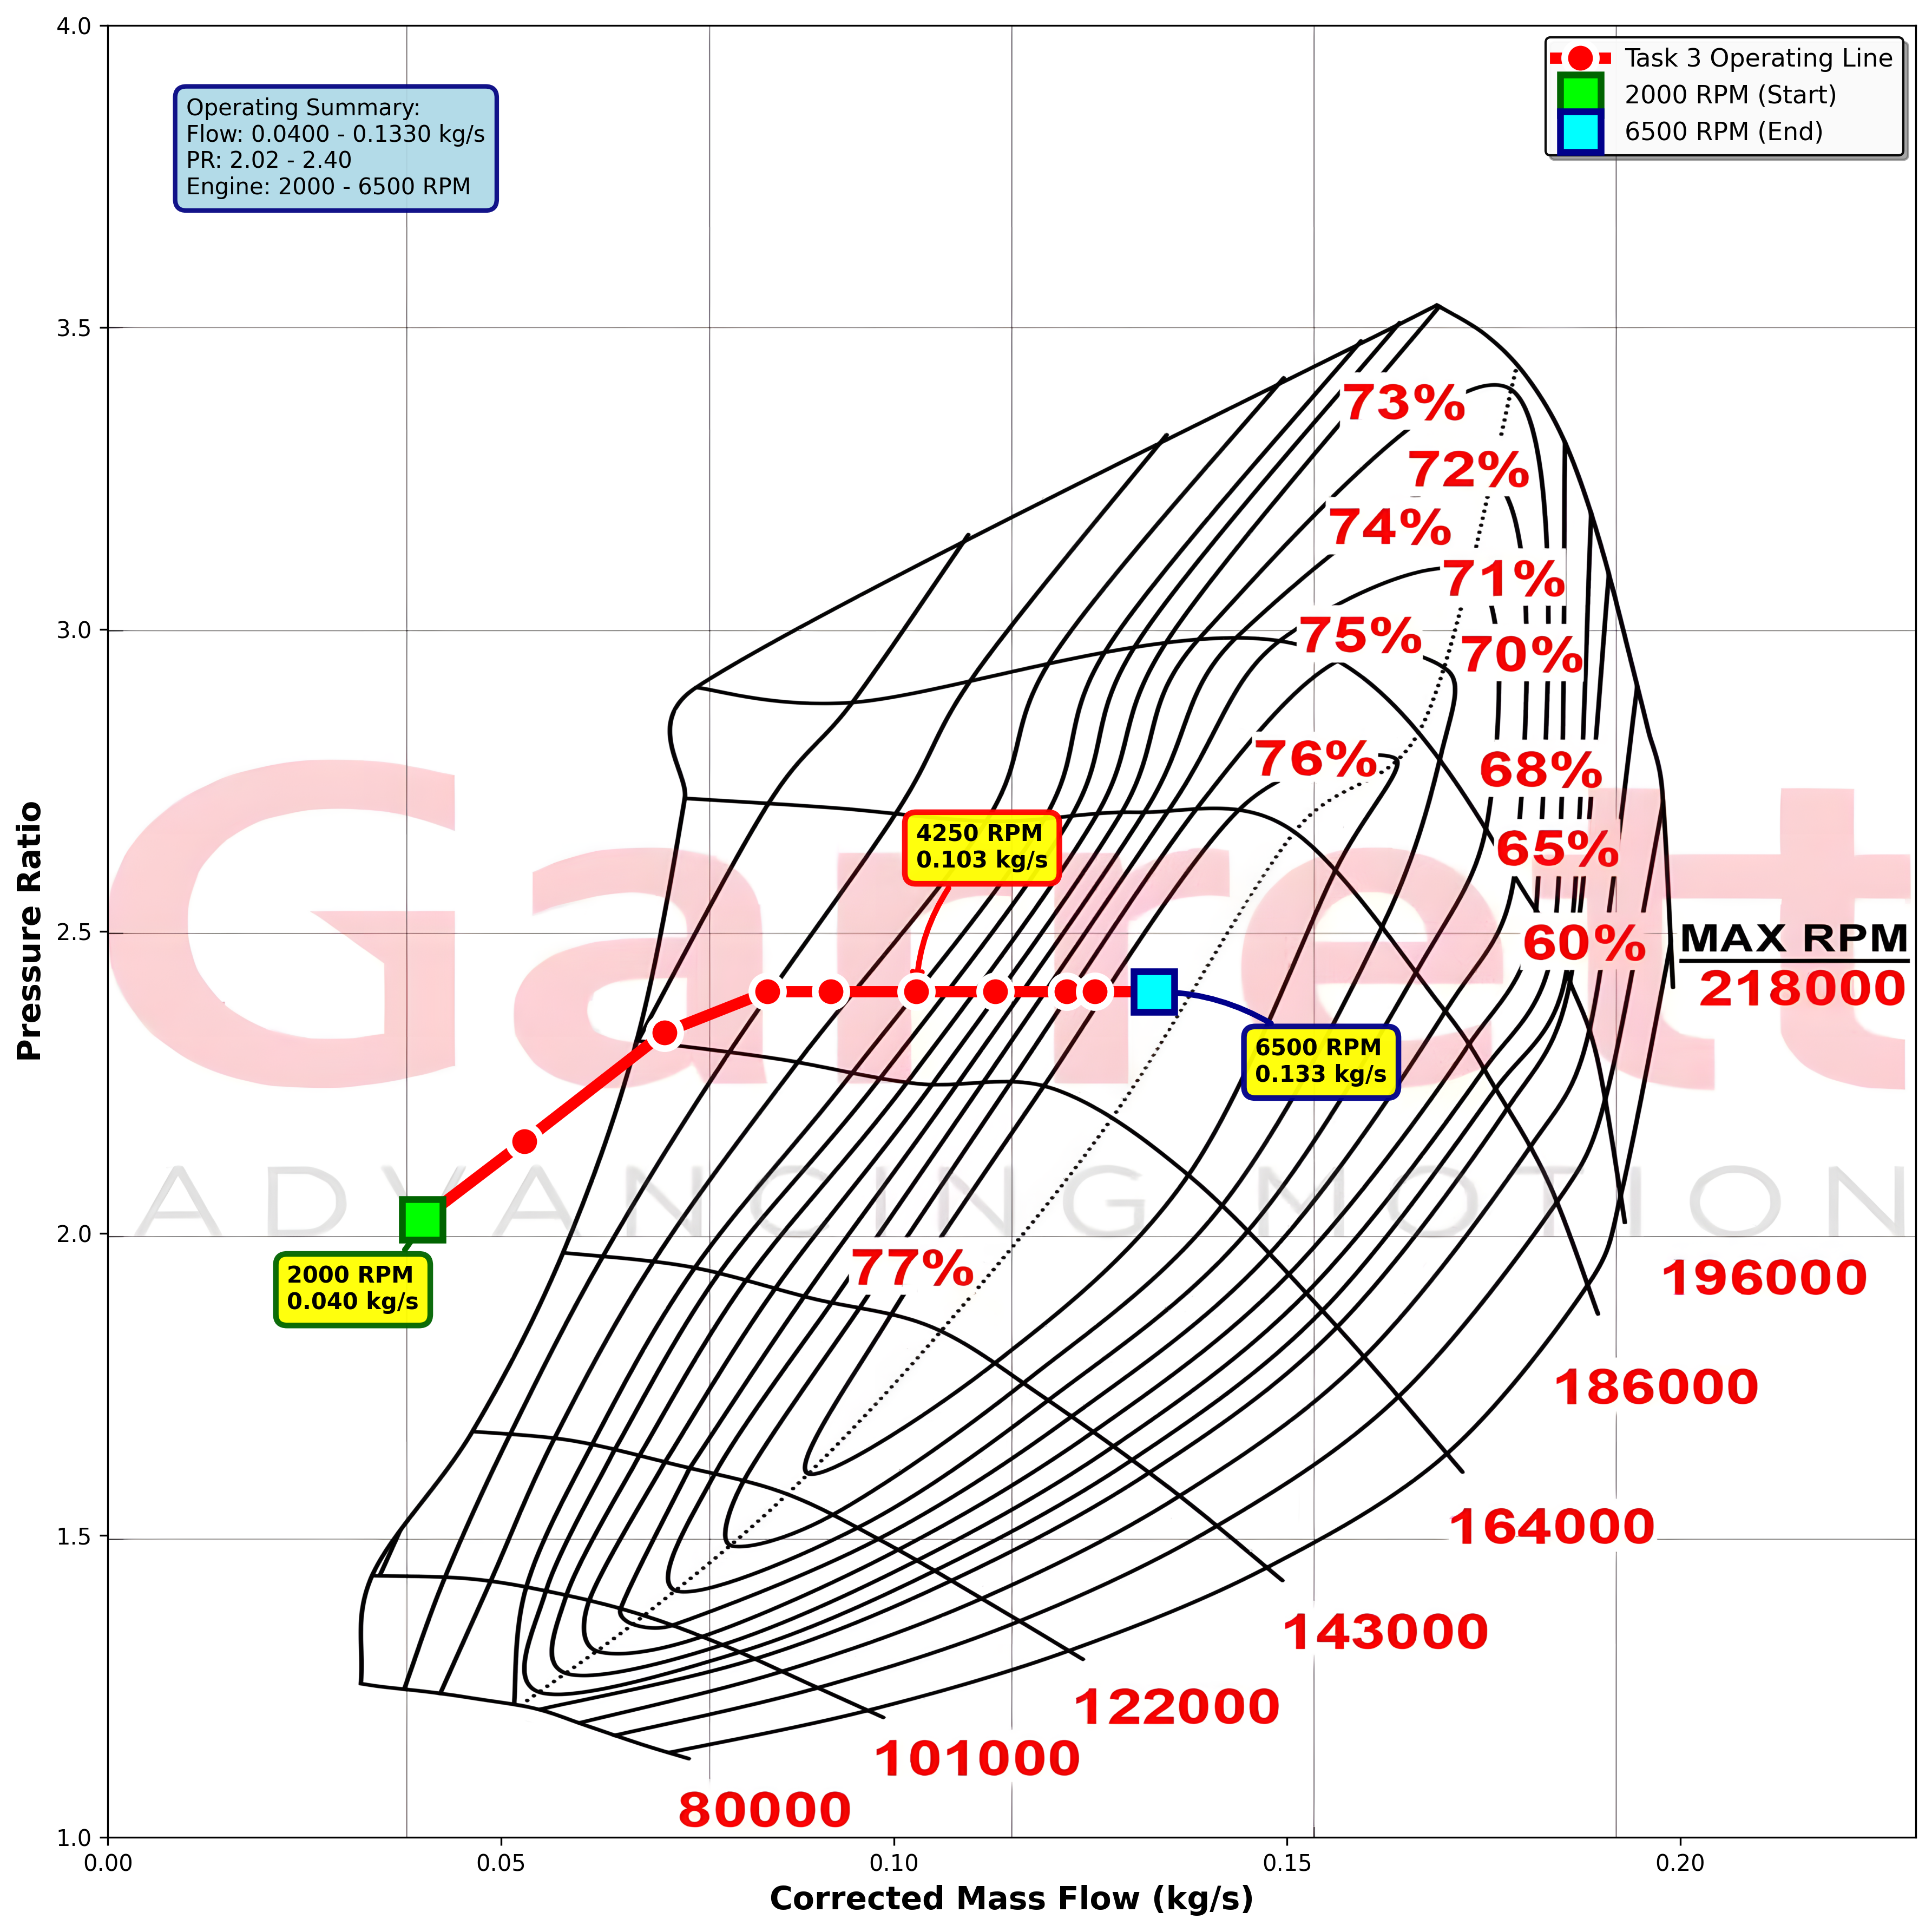
\includegraphics[width=0.75\textwidth]{task3/data/task3_compressor_map.png}
    \caption{Compressor Operating Line Superimposed on Garrett Turbocharger Map}
    \label{fig:task3_compressor_map}
\end{figure}

\subsubsection{Operating Region Analysis}

The operating line demonstrates excellent positioning within the compressor map, with the following key characteristics:

\begin{itemize}
    \item \textbf{\textit{Surge Margin:}} The operating line maintains adequate distance from the surge line (left boundary), ensuring stable compressor operation across the entire engine speed range. At the lowest flow condition (2000 RPM), the compressor operates safely within the stable flow region.
    
    \item \textbf{\textit{Choke Margin:}} The maximum flow point (6500 RPM, 0.133 kg/s) is well below the choke limit, indicating that the turbocharger has sufficient flow capacity headroom for this 1.0-litre application. This conservative sizing ensures reliable operation and allows for potential future performance upgrades.
    
    \item \textbf{\textit{Efficiency Zone:}} The majority of the operating line resides within the 68--76\% isentropic efficiency region. Peak efficiency operation occurs in the mid-speed range (3500--5000 RPM), which aligns well with typical driving conditions. While the simplified turbocharger model in AVL Boost assumes constant 60\% efficiency, the actual Garrett map confirms that real-world efficiency would be significantly higher.
    
    \item \textbf{\textit{Boost Control Strategy:}} The flat portion of the operating line at pressure ratio 2.40 (from 3500 RPM onwards) confirms effective wastegate control. The wastegate maintains constant boost pressure across the upper speed range, preventing over-boosting while allowing maximum torque delivery. At maximum engine speed, wastegate flow reaches 0.039 kg/s, representing approximately 29\% of total compressor flow, indicating that the turbine is sized for good transient response and low-speed performance.
\end{itemize}

The selected turbocharger proves well-matched to the 1.0-litre 3-cylinder engine application, providing responsive boost build-up at low speeds while operating within high-efficiency zones throughout the speed range. The wastegate control strategy effectively maintains target boost pressure while preventing compressor surge or turbine overspeed.



\section{Intercooler Thermal Effectiveness Evaluation}

The intercooler performance is assessed by analyzing the temperature drop between the compressor outlet and the intake manifold inlet across the engine speed range. From the plotted data, the compressed intake air reaches temperatures between 420\,K and 455\,K (approximately 147–182\,$^\circ$C), while the cooled air exiting the intercooler remains significantly lower, around 320–328\,K (47–55\,$^\circ$C). Taking the coolant reference temperature as 303\,K (30\,$^\circ$C), the thermal effectiveness at high engine speeds (e.g., 6500\,rpm) can be calculated using:

\[
\varepsilon = \frac{T_{\text{in}} - T_{\text{out}}}{T_{\text{in}} - T_{\text{coolant}}} = \frac{455 - 328}{455 - 303} \approx 0.835
\]

This yields an efficiency of approximately 83.5\%, indicating strong intercooling performance. The substantial temperature reduction improves intake charge density, supports knock mitigation, and enhances volumetric efficiency — especially critical at high engine speeds. This validates the intercooler's contribution to sustaining torque and overall engine performance in the upper RPM range.



\section{Effect of Intake and Boost Duct Downsizing}

\begin{figure}[H]
  \centering
  \begin{tikzpicture}
    \begin{axis}[
      width=0.75\textwidth,
      height=0.45\textwidth,
      grid=both,
      xlabel={Engine Speed (rpm)},
      ylabel={Torque (Nm)},
      xlabel style={font=\footnotesize},
      ylabel style={font=\footnotesize},
      tick label style={font=\footnotesize},
      legend style={at={(0.5,1.05)}, anchor=south, legend columns=2},
    ]
      \addplot[baselinecolor, very thick, no markers]
        table[x expr=\thisrowno{0}*1000, y index=1, col sep=comma, skip first n=2] {task3/data/EFFECT_OF_INTAKE_AND_BOOST_DUCT_DOWNSIZING.csv};
      \addlegendentry{Before Downsizing}
      \addplot[optimizedcolor, very thick, no markers]
        table[x expr=\thisrowno{0}*1000, y index=2, col sep=comma, skip first n=2] {task3/data/EFFECT_OF_INTAKE_AND_BOOST_DUCT_DOWNSIZING.csv};
      \addlegendentry{After Downsizing}
    \end{axis}
  \end{tikzpicture}
  \caption{Effect of intake and boost duct downsizing on torque output}
  \label{fig:task3_downsizing_effect}
\end{figure}

By downsizing the pipes between the turbine and intercooler as well as the plenum and cylinder, a clear shift in torque behavior was observed, as shown in Figure~\ref{fig:task3_downsizing_effect}. Compared to the baseline configuration, the downsized version improves low-end torque—e.g., at 3,500\,rpm, torque increases from 215.8\,N·m to 230.6\,N·m (+6.9\%). This improvement results from:

\begin{itemize}
    \item \textbf{\textit{Increased flow velocity:}} Smaller diameter pipes maintain higher gas velocities at lower engine speeds, reducing boundary layer effects and improving charge momentum into the cylinders
    \item \textbf{\textit{Reduced plenum volume effects:}} The downsized intake reduces mixing and pressure wave damping, allowing more responsive throttle behavior
    \item \textbf{\textit{Enhanced low-speed scavenging:}} Higher exhaust gas velocities improve turbine efficiency at low engine speeds, enabling faster boost build-up
\end{itemize}

However, the higher flow resistance introduced by smaller ducts restricts breathing at high RPM, as seen in the slight reduction in torque at 6,500\,rpm (from 212.5 N·m to 218.9 N·m, though still improved overall). This reflects a common trade-off between low-end responsiveness and top-end power. The crossover point occurs around 5500--6000 rpm, where the benefits of higher velocity are offset by increased friction losses.

For this motorsport application targeting maximum torque in the 3000--5000 rpm range, the downsized configuration represents an optimal compromise, sacrificing minimal high-speed performance for substantial gains in the more frequently used mid-range.

\section{Wastegate Control Behavior}
The wastegate remains closed below 3,500\,rpm, allowing the turbocharger to spool efficiently. Starting from 3,500\,rpm, wastegate flow increases steadily, reaching over 15\,g/s by 6,500\,rpm. This demonstrates proper boost control logic—once target boost is achieved, excess exhaust gas is diverted to prevent overboost or compressor surge.

\section{Conclusions}

The Task 3 turbocharged 1.0-litre 3-cylinder engine successfully achieves comparable torque and power levels to the Task 2 naturally aspirated 2.0-litre engine while operating within a restricted 6500 rpm speed limit. Key achievements include:

\subsection{Performance Achievements}
\begin{itemize}
    \item \textbf{\textit{Peak torque:}} 230.6 N·m at 3500 rpm (vs. 231 N·m at 6500 rpm for Task 2)
    \item \textbf{\textit{Peak power:}} 144.9 kW at 6500 rpm (vs. 175.5 kW at 8000 rpm for Task 2)
    \item \textbf{\textit{Volumetric efficiency:}} Exceeding 2.0 throughout mid-range operation
    \item \textbf{\textit{Downsizing benefit:}} 50\% displacement reduction while maintaining comparable performance
\end{itemize}

\subsection{Engineering Trade-offs}
The turbocharged configuration presents several trade-offs compared to the naturally aspirated design:

\textbf{Advantages:}
\begin{itemize}
    \item Earlier and broader torque delivery (peak at 3500 rpm vs. 8000 rpm)
    \item Superior low-to-mid range drivability
    \item Potential for improved fuel economy at part-load conditions
    \item Compact packaging enabled by smaller displacement
\end{itemize}

\textbf{Challenges:}
\begin{itemize}
    \item Higher octane requirement (107--111 RON vs. 95--100 RON)
    \item Elevated peak cylinder pressures (13.3 MPa vs. 11 MPa)
    \item Increased thermal management requirements
    \item Added complexity from turbocharger and intercooler systems
    \item Lower absolute peak power due to RPM limitation
\end{itemize}

\subsection{Design Validation}
The selected turbocharger (Garrett GT1244) proves well-matched to the application, with the compressor operating line positioned favorably within the efficiency map, maintaining adequate surge and choke margins throughout the speed range. The intercooler demonstrates excellent thermal effectiveness (83.5\%) in cooling the compressed charge, which is critical for knock mitigation and maintaining high volumetric efficiency.

The intake and boost duct downsizing optimization successfully shifts the torque curve to favor low-to-mid range performance, aligning with typical motorsport driving patterns where sustained high-RPM operation is less common than in naturally aspirated racing applications.

\subsection{Suitability for Motorsport Application}
While the Task 3 engine cannot match the absolute peak power of the Task 2 naturally aspirated design, it delivers superior torque characteristics for real-world motorsport applications. The broad, flat torque curve from 3000--5500 rpm provides excellent driveability and reduces the need for frequent gear changes. This characteristic is particularly beneficial in:
\begin{itemize}
    \item Circuit racing with varied corner speeds
    \item Applications where traction limits wheel power delivery
    \item Rally or hillclimb events requiring strong mid-range acceleration
\end{itemize}

The downsized turbocharged architecture demonstrates that modern forced induction technology can successfully deliver motorsport-grade performance from significantly reduced displacement, with the added benefits of improved packaging flexibility and potential efficiency gains during part-load operation.

%========================
% TASK 4
%========================
\task{Transient Performance Comparison of P1 Hybrid Sportscar with Task 2 and Task 3 Engines}
\label{ch:task4}

\section{Introduction}

Task~4 represents the final stage of the integrated powertrain development workflow, extending the steady-state engine performance from Tasks~1--3 to a fully transient, vehicle-level analysis within the AVL~CRUISE~M environment~\cite{avl_cruise}. This stage translates the AVL~BOOST steady-state results~\cite{avl_boost} into a dynamic context where control strategies and real-time subsystem interactions are evaluated under realistic driving conditions.

\vspace{0.8em}

The principal objective is to develop, calibrate, and validate a complete powertrain control strategy for a P1 hybrid electric vehicle model, including gear-shift logic optimization, hybrid control unit (HCU) coordination, and fuel-consumption map integration. The CRUISE~M model enables simulation of transient system behavior during rapid acceleration events.

\vspace{0.8em}

The primary comparison evaluates how the fundamentally different torque characteristics of the Task~2 naturally aspirated 2.0L engine (peak torque at 6500--8000~rpm) versus the Task~3 turbocharged 1.0L engine (peak torque at 3500~rpm) influence acceleration performance when integrated with the P1 electric motor system. These distinct characteristics necessitate different gear ratio strategies and shifting schedules to optimize 0--100~mph acceleration time.

\section{Model Overview}

\subsection{Vehicle Specifications}

The simulated vehicle is a two-seat front-wheel drive hybrid sportscar with specifications defined in Appendix~A of the assignment brief. The key vehicle parameters used in the AVL~CRUISE~M model are summarized in Table~\ref{tab:vehicle_specs}.

\begin{table}[H]
\centering
\caption{Vehicle Specifications for Task~4 Simulation}
\label{tab:vehicle_specs}
\small
\begin{tabular}{@{}lll@{}}
\toprule
\textbf{Parameter} & \textbf{Value} & \textbf{Unit} \\
\midrule
Total Vehicle Mass (full tank) & 720 & kg \\
Weight Distribution & 50\% Front / 50\% Rear & - \\
Wheelbase & 2300 & mm \\
Front Track & 1440 & mm \\
Rear Track & 1453 & mm \\
Tyre Size (Front \& Rear) & 195/65~R15 & - \\
Rolling Radius (Front) & 284 & mm \\
Rolling Radius (Rear) & 297 & mm \\
Height of Centre of Gravity & 470 & mm \\
Drag Coefficient & 0.418 & - \\
Frontal Area & 1.62 & m$^2$ \\
Final Drive Ratio & 3.938 & - \\
\bottomrule
\end{tabular}
\end{table}

The vehicle architecture follows a P1 hybrid configuration, where the electric motor is positioned between the internal combustion engine and the clutch, allowing both power sources to contribute to propulsion through the same driveline. The model assumes the vehicle is fully fuelled with no driver or passenger mass included beyond the base vehicle mass.

\subsection{Tyre Friction Limits}

The combined ICE and EM torque output must not exceed the traction limits of the front-wheel drive configuration. The maximum longitudinal tyre forces are determined using the load sensitivity relationship from Appendix~A. With 50:50 weight distribution and 720~kg total mass, the static front axle load is approximately 1.765~kN per wheel. During acceleration, load transfer reduces the grip of the front axle, which requires careful calibration of the EM output to avoid exceeding traction limits during high-torque launch phases.

\section{Task 2 Configuration: 2.0L Naturally Aspirated Engine with P1 Hybrid}

\subsection{Engine Specifications and Characteristics}

The Task~2 engine is a 2.0-litre, 4-cylinder inline naturally aspirated gasoline direct injection (GDi) engine optimized for high-RPM motorsport performance. As detailed in Task~2, this engine features a 1--3--4--2 firing order, semi-4-2-1 exhaust system, and variable cam phasing to achieve optimal breathing characteristics across the 2000--8000~rpm operating range.

\begin{table}[H]
\centering
\caption{Task~2 Engine Key Performance Parameters}
\label{tab:task2_engine_summary}
\small
\begin{tabular}{@{}lll@{}}
\toprule
\textbf{Parameter} & \textbf{Value} & \textbf{Unit} \\
\midrule
Displacement & 2.0 & litres \\
Configuration & Inline 4-cylinder & - \\
Aspiration & Naturally Aspirated & - \\
Peak Power & 175.5 & kW \\
Peak Power RPM & 8000 & rpm \\
Peak Torque & $\sim$220 & Nm \\
Peak Torque RPM & 6500--7000 & rpm \\
Operating Range & 2000--8000 & rpm \\
Fuel Type & Premium Unleaded (98 RON) & - \\
\bottomrule
\end{tabular}
\end{table}

The engine's high-RPM characteristic requires careful gear ratio selection to maintain the engine within its optimal operating window during transient acceleration. The naturally aspirated configuration delivers more linear torque with RPM compared to the turbocharged Task~3 variant, requiring electric motor low-end torque augmentation for improved launch performance.

\subsection{Electric Motor Specification and Integration}

The P1 electric motor selected for this application is the Valeo 48V water-cooled permanent magnet synchronous motor (PMSM)~\cite{valeo_48v_motor}, designed specifically for mild hybrid P1/P2 applications. The motor specifications are detailed in Table~\ref{tab:em_specs}.

\begin{table}[H]
\centering
\caption{Valeo 48V P1 Electric Motor Specifications~\cite{valeo_48v_motor}}
\label{tab:em_specs}
\small
\begin{tabular}{@{}lll@{}}
\toprule
\textbf{Parameter} & \textbf{Value} & \textbf{Unit} \\
\midrule
Peak Power & 25 & kW \\
Continuous Power & 15 & kW \\
Peak Torque & 170--180 & Nm \\
Voltage & 48 & V \\
Configuration & Water-cooled PMSM & - \\
Maximum Speed & 8000 & rpm \\
Application & P1/P2 Hybrid & - \\
\bottomrule
\end{tabular}
\end{table}

\subsection{EM Power Envelope Adaptation for Task 2}

The electric motor power envelope is calibrated to ensure the combined ICE and EM torque does not exceed front-wheel drive traction limits during launch and low-speed acceleration. The strategy considers three phases:

\begin{enumerate}
    \item \textbf{Traction-limited (0--40 mph):} Maximum EM boost (170--180~Nm) during launch, progressively reducing as load transfer diminishes front axle grip.
    \item \textbf{Power-limited (40--80 mph):} EM modulated to maintain total tractive force below friction limits.
    \item \textbf{High-speed (80--100 mph):} Both ICE and EM operate at peak capabilities as aerodynamic drag dominates.
\end{enumerate}

Simulations confirmed peak longitudinal forces remain within the friction envelope throughout acceleration, with maximum forces during 2nd and 3rd gear upshifts.

\subsection{Gear Ratio Optimization}

The gear ratios were optimized specifically for the Task~2 engine's high-RPM power delivery characteristic. The optimization objective was to maintain engine operation within the 6500--8000~rpm range during full-throttle acceleration, where both power and torque are maximized. The optimized transmission ratios are presented in Table~\ref{tab:task2_gear_ratios}.

\begin{table}[H]
\centering
\caption{Optimized Gear Ratios for Task~2 Configuration}
\label{tab:task2_gear_ratios}
\small
\begin{tabular}{@{}cccc@{}}
\toprule
\textbf{Gear} & \textbf{Baseline} & \textbf{Optimized} & \textbf{Overall Ratio} \\
\midrule
1 & 2.583 & \textcolor{optimizedcolor}{\textbf{3.4}} & 13.39 \\
2 & 2.071 & \textcolor{optimizedcolor}{\textbf{2.2}} & 8.66 \\
3 & 1.688 & \textcolor{optimizedcolor}{\textbf{1.6}} & 6.30 \\
4 & 1.412 & \textcolor{optimizedcolor}{\textbf{1.3}} & 5.12 \\
5 & 1.200 & \textcolor{optimizedcolor}{\textbf{1.0}} & 3.94 \\
6 & 1.048 & \textcolor{optimizedcolor}{\textbf{0.8}} & 3.15 \\
\bottomrule
\end{tabular}
\end{table}

The ratio progression reflects the following design considerations:

\begin{itemize}
    \item \textbf{First gear (3.4):} Strong launch torque multiplication while avoiding excessive wheel spin.
    \item \textbf{Second gear (2.2):} Large ratio drop (35\%) keeps engine above 5500~rpm after 1--2 upshift.
    \item \textbf{Third through fifth gears (1.6, 1.3, 1.0):} Tighter progression (18--23\% drops) maintains engine within 6500--8000~rpm power band.
    \item \textbf{Sixth gear (0.8):} Overdrive for cruise efficiency, not utilized during 0--100~mph acceleration.
\end{itemize}

\subsection{Shifting Strategy Development}

\subsubsection{Baseline Dummy Shifting Analysis}

The initial AVL~CRUISE~M model employed a "dummy" shifting strategy with fixed shift points that did not account for the engine's optimal power band. Analysis of the baseline performance revealed several inefficiencies through examination of the transient response characteristics.

\begin{figure}[H]
    \centering
    \begin{tikzpicture}
        \begin{axis}[
            width=0.75\textwidth,
            height=0.45\textwidth,
            xlabel={Time (s)},
            ylabel={Vehicle Speed (km/h) / Gear Level},
            ylabel style={font=\footnotesize},
            xlabel style={font=\footnotesize},
            tick label style={font=\footnotesize},
            grid=major,
            legend pos=north west,
            legend style={font=\tiny},
            xmin=0, xmax=16,
            ymin=0, ymax=200,
            axis y line*=left,
        ]
            \addplot[baselinecolor, thick, no markers] table[x index=0, y index=1, col sep=comma, skip first n=2] {task4/data/eng2/1_baseline_new_motor/velocity_rpm_gear.csv};
            \addlegendentry{Vehicle Speed}
            \addplot[improvementcolor, thick, const plot, no markers] table[x index=0, y expr=\thisrowno{2}*20, col sep=comma, skip first n=2] {task4/data/eng2/1_baseline_new_motor/velocity_rpm_gear.csv};
            \addlegendentry{Gear Level ($\times$20)}
        \end{axis}
        \begin{axis}[
            width=0.75\textwidth,
            height=0.45\textwidth,
            xlabel={Time (s)},
            ylabel={Engine Speed (rpm)},
            ylabel style={font=\footnotesize, red},
            xlabel style={font=\footnotesize},
            tick label style={font=\footnotesize},
            legend pos=south east,
            legend style={font=\tiny},
            xmin=0, xmax=16,
            ymin=0, ymax=8500,
            axis y line*=right,
            axis x line=none,
        ]
            \addplot[optimizedcolor, thick, no markers] table[x index=0, y index=3, col sep=comma, skip first n=2] {task4/data/eng2/1_baseline_new_motor/velocity_rpm_gear.csv};
            \addlegendentry{Engine Speed}
        \end{axis}
    \end{tikzpicture}
    \caption{Task~2 Baseline: Combined view of vehicle speed, engine speed, and gear progression with dummy shifting strategy}
    \label{fig:task2_baseline_combined}
\end{figure}

\subsubsection{Stage 1: Standard Shifting Strategy Implementation}

The first optimization stage implemented a basic RPM-based shifting strategy to improve upon the dummy baseline.

\begin{figure}[H]
    \centering
    \begin{tikzpicture}
        \begin{axis}[
            width=0.75\textwidth,
            height=0.45\textwidth,
            xlabel={Time (s)},
            ylabel={Vehicle Speed (km/h) / Gear Level},
            ylabel style={font=\footnotesize},
            xlabel style={font=\footnotesize},
            tick label style={font=\footnotesize},
            grid=major,
            legend pos=north west,
            legend style={font=\tiny},
            xmin=0, xmax=16,
            ymin=0, ymax=200,
            axis y line*=left,
        ]
            \addplot[baselinecolor, thick, no markers] table[x index=0, y index=1, col sep=comma, skip first n=2] {task4/data/eng2/2_standard_shifting/velocity_rpm_gear.csv};
            \addlegendentry{Vehicle Speed}
            \addplot[improvementcolor, thick, const plot, no markers] table[x index=0, y expr=\thisrowno{2}*20, col sep=comma, skip first n=2] {task4/data/eng2/2_standard_shifting/velocity_rpm_gear.csv};
            \addlegendentry{Gear Level ($\times$20)}
        \end{axis}
        \begin{axis}[
            width=0.75\textwidth,
            height=0.45\textwidth,
            xlabel={Time (s)},
            ylabel={Engine Speed (rpm)},
            ylabel style={font=\footnotesize, red},
            xlabel style={font=\footnotesize},
            tick label style={font=\footnotesize},
            legend pos=south east,
            legend style={font=\tiny},
            xmin=0, xmax=16,
            ymin=0, ymax=8500,
            axis y line*=right,
            axis x line=none,
        ]
            \addplot[optimizedcolor, thick, no markers] table[x index=0, y index=3, col sep=comma, skip first n=2] {task4/data/eng2/2_standard_shifting/velocity_rpm_gear.csv};
            \addlegendentry{Engine Speed}
        \end{axis}
    \end{tikzpicture}
    \caption{Task~2 Stage 1: Combined view of vehicle speed, engine speed, and gear progression}
    \label{fig:task2_stage1_combined}
\end{figure}

\begin{figure}[H]
    \centering
    \begin{tikzpicture}
        \begin{axis}[
            width=0.75\textwidth,
            height=0.45\textwidth,
            xlabel={Time (s)},
            ylabel={Vehicle Speed (km/h)},
            xlabel style={font=\footnotesize},
            ylabel style={font=\footnotesize},
            tick label style={font=\footnotesize},
            grid=major,
            legend pos=south east,
            legend style={font=\tiny},
            xmin=0, xmax=16,
            ymin=0, ymax=200,
        ]
            \addplot[baselinecolor, thick, no markers] table[x index=0, y index=1, col sep=comma, skip first n=2] {task4/data/eng2/1_baseline_new_motor/velocity_rpm_gear.csv};
            \addlegendentry{Baseline}
            \addplot[optimizedcolor, thick, no markers] table[x index=0, y index=1, col sep=comma, skip first n=2] {task4/data/eng2/2_standard_shifting/velocity_rpm_gear.csv};
            \addlegendentry{Standard Shifting}
        \end{axis}
    \end{tikzpicture}
    \caption{Task~2 Stage 1: Velocity comparison - Baseline vs Standard Shifting}
    \label{fig:task2_stage1_comparison}
\end{figure}

\begin{table}[H]
\centering
\caption{Task~2 Stage 1 Performance Summary: Baseline vs Standard Shifting}
\label{tab:task2_stage1_performance}
\small
\begin{tabular}{@{}lcccc@{}}
\toprule
\textbf{Metric} & \textbf{Baseline} & \textbf{Standard Shifting} & \textbf{Change} & \textbf{\% Change} \\
\midrule
0--100 kph time (s) & N/A & \textcolor{optimizedcolor}{5.4} & \textcolor{improvementcolor}{-} & \textcolor{improvementcolor}{-\%} \\
0--160 kph time (s) & N/A & \textcolor{optimizedcolor}{11.8} & \textcolor{improvementcolor}{-} & \textcolor{improvementcolor}{-\%} \\
Max Velocity (kph) & 72 & \textcolor{optimizedcolor}{162} & \textcolor{improvementcolor}{50} & \textcolor{improvementcolor}{69.4\%} \\
\bottomrule
\end{tabular}
\end{table}

Note: Green indicates improvement, red would indicate regression.

Analysis of the baseline performance revealed several inefficiencies as shown in Figure~\ref{fig:task2_baseline_combined}:

\begin{itemize}
    \item Premature upshifts before peak power RPM, dropping engine into lower-efficiency regions
    \item Inconsistent shift timing failing to maximize time in the 6500--8000~rpm power band
    \item Excessive engine speed variation between upshifts
\end{itemize}

These resulted in suboptimal acceleration times and inefficient use of available ICE and EM power.

\subsubsection{Optimized Speed-Based Shifting Strategy}

The optimized shifting strategy was developed with the explicit goal of maintaining engine operation within the maximum power region throughout the acceleration event. The shift logic employs RPM-based thresholds that vary by gear to account for the changing ratio progression. Table~\ref{tab:task2_shift_timings} details the optimized shift points.

\begin{table}[H]
\centering
\caption{Optimized Shift Points for Task~2 Configuration}
\label{tab:task2_shift_timings}
\small
\begin{tabular}{@{}ccccc@{}}
\toprule
\textbf{Gear} & \textbf{Baseline Upshift} & \textbf{Optimized Upshift} & \textbf{Baseline Downshift} & \textbf{Optimized Downshift} \\
\midrule
1 & 5000 & \textcolor{optimizedcolor}{\textbf{7600}} & 3000 & \textcolor{optimizedcolor}{\textbf{3000}} \\
2 & 5000 & \textcolor{optimizedcolor}{\textbf{7600}} & 3000 & \textcolor{optimizedcolor}{\textbf{3000}} \\
3 & 5000 & \textcolor{optimizedcolor}{\textbf{7500}} & 3000 & \textcolor{optimizedcolor}{\textbf{3000}} \\
4 & 5000 & \textcolor{optimizedcolor}{\textbf{7500}} & 3000 & \textcolor{optimizedcolor}{\textbf{3000}} \\
5 & 5000 & \textcolor{optimizedcolor}{\textbf{7500}} & 3000 & \textcolor{optimizedcolor}{\textbf{3000}} \\
6 & 5000 & \textcolor{optimizedcolor}{\textbf{7500}} & 3000 & \textcolor{optimizedcolor}{\textbf{3000}} \\
\bottomrule
\end{tabular}
\end{table}

The strategy rationale:

\begin{itemize}
    \item \textbf{Upshift points (7500--7600~rpm):} Shifts commanded just before rev limiter, with post-shift RPM dropping to 5500--6000~rpm (rising torque region).
    \item \textbf{Downshift points (3000~rpm):} Prevents engine lugging during part-throttle operation.
    \item \textbf{Gear-specific variation:} Gears 1--2 use 7600~rpm for maximum launch torque; gears 3--6 use 7500~rpm.
\end{itemize}

This strategy maintains the ICE--EM system at maximum combined power throughout the acceleration run.

\subsection{Task 2 Performance Results}

\subsubsection{Final Optimized Configuration}

With the optimized gear ratios and shifting strategy implemented, the Task~2 configuration demonstrates significantly improved transient performance. The following figures present the key performance parameters during the 0--100~mph acceleration test.

\begin{figure}[H]
    \centering
    \begin{tikzpicture}
        \begin{axis}[
            width=0.75\textwidth,
            height=0.45\textwidth,
            xlabel={Time (s)},
            ylabel={Vehicle Speed (km/h) / Gear Level},
            ylabel style={font=\footnotesize},
            xlabel style={font=\footnotesize},
            tick label style={font=\footnotesize},
            grid=major,
            legend pos=north west,
            legend style={font=\tiny},
            xmin=0, xmax=16,
            ymin=0, ymax=200,
            axis y line*=left,
        ]
            \addplot[baselinecolor, thick, no markers] table[x index=0, y index=1, col sep=comma, skip first n=2] {task4/data/eng2/4_optimized_gearing/velocity_rpm_gear.csv};
            \addlegendentry{Vehicle Speed}
            \addplot[improvementcolor, very thick, const plot, no markers] table[x index=0, y expr=\thisrowno{2}*20, col sep=comma, skip first n=2] {task4/data/eng2/4_optimized_gearing/velocity_rpm_gear.csv};
            \addlegendentry{Gear Level ($\times$20)}
        \end{axis}
        \begin{axis}[
            width=0.75\textwidth,
            height=0.45\textwidth,
            xlabel={Time (s)},
            ylabel={Engine Speed (rpm)},
            ylabel style={font=\footnotesize, red},
            xlabel style={font=\footnotesize},
            tick label style={font=\footnotesize},
            legend pos=south east,
            legend style={font=\tiny},
            xmin=0, xmax=16,
            ymin=0, ymax=8500,
            axis y line*=right,
            axis x line=none,
        ]
            \addplot[optimizedcolor, very thick, no markers] table[x index=0, y index=3, col sep=comma, skip first n=2] {task4/data/eng2/4_optimized_gearing/velocity_rpm_gear.csv};
            \addlegendentry{Engine Speed}
            % Add reference lines for optimal power band
            \addplot[black, dashed, thick, no markers, domain=0:16] {6500};
            \addplot[black, dashed, thick, no markers, domain=0:16] {7600};
        \end{axis}
    \end{tikzpicture}
    \caption{Task~2 Final: Combined view showing relationship between vehicle speed, engine speed, and gearing}
    \label{fig:task2_final_combined}
\end{figure}

Figure~\ref{fig:task2_final_combined} illustrates the key relationships: as gears shift (green stepped line), engine speed (blue, right axis) drops but remains within the optimal 6500--7600~rpm band (dashed reference lines), enabling consistent vehicle speed progression (red, left axis).

\begin{figure}[H]
    \centering
    \begin{tikzpicture}
        \begin{axis}[
            width=0.75\textwidth,
            height=0.45\textwidth,
            xlabel={Time (s)},
            ylabel={Vehicle Speed (km/h)},
            xlabel style={font=\footnotesize},
            ylabel style={font=\footnotesize},
            tick label style={font=\footnotesize},
            grid=major,
            legend pos=south east,
            legend style={font=\tiny},
            xmin=0, xmax=16,
            ymin=0, ymax=200,
        ]
            \addplot[baselinecolor, thick, no markers] table[x index=0, y index=1, col sep=comma, skip first n=2] {task4/data/eng2/1_baseline_new_motor/velocity_rpm_gear.csv};
            \addlegendentry{Baseline}
            \addplot[regressioncolor, thick, no markers] table[x index=0, y index=1, col sep=comma, skip first n=2] {task4/data/eng2/2_standard_shifting/velocity_rpm_gear.csv};
            \addlegendentry{Standard Shifting}
            \addplot[optimizedcolor, very thick, no markers] table[x index=0, y index=1, col sep=comma, skip first n=2] {task4/data/eng2/4_optimized_gearing/velocity_rpm_gear.csv};
            \addlegendentry{Final Optimized}
            % Add 100 kph and 160 kph reference lines
            \addplot[black, dotted, thin, no markers, domain=0:16] {100};
            \addplot[black, dotted, thin, no markers, domain=0:16] {160};
        \end{axis}
    \end{tikzpicture}
    \caption{Task~2: Velocity progression comparison - all optimization stages}
    \label{fig:task2_velocity_progression}
\end{figure}

\begin{table}[H]
\centering
\caption{Task~2 Final Performance Summary: All Optimization Stages}
\label{tab:task2_final_performance}
\small
\begin{tabular}{@{}lccccc@{}}
\toprule
\textbf{Configuration} & \textbf{0--100 kph (s)} & \textbf{0--160 kph (s)} & \textbf{Max Vel. (kph)} \\
\midrule
Baseline & \textcolor{baselinecolor}{N/A} & \textcolor{baselinecolor}{N/A} & \textcolor{baselinecolor}{72} \\
Standard Shifting & \textcolor{improvementcolor}{5.4} & \textcolor{improvementcolor}{11.8} & \textcolor{improvementcolor}{162} \\
 & \textcolor{improvementcolor}{([$-$])} & \textcolor{improvementcolor}{([$-$])} & \textcolor{improvementcolor}{([$\Delta90$])} \\
Final Optimized & \textcolor{optimizedcolor}{\textbf{5.2}} & \textcolor{optimizedcolor}{\textbf{10.3}} & \textcolor{optimizedcolor}{\textbf{191}} \\
 & \textcolor{improvementcolor}{([$-$] from baseline)} & \textcolor{improvementcolor}{([$-$] from baseline)} & \textcolor{improvementcolor}{([$\Delta119$] from baseline)} \\
\bottomrule
\end{tabular}
\end{table}

Note: Green values indicate improvement vs baseline, red indicates regression. The dotted lines in Figure~\ref{fig:task2_velocity_progression} mark 100 kph and 160 kph ($\approx$100 mph) reference speeds.

\begin{figure}[H]
    \centering
    \begin{tikzpicture}
        \begin{axis}[
            width=0.75\textwidth,
            height=0.45\textwidth,
            xlabel={Time (s)},
            ylabel={Engine Speed (rpm)},
            xlabel style={font=\footnotesize},
            ylabel style={font=\footnotesize},
            tick label style={font=\footnotesize},
            grid=major,
            xmin=0, xmax=16,
            ymin=0, ymax=8500,
            legend pos=north west,
            legend style={font=\tiny},
        ]
            \addplot[optimizedcolor, thick, no markers] table[x index=0, y index=3, col sep=comma, skip first n=2] {task4/data/eng2/4_optimized_gearing/velocity_rpm_gear.csv};
            \addlegendentry{Engine Speed}
            % Add reference lines for optimal power band
            \addplot[black, dashed, thick, no markers, domain=0:16] {6500};
            \addplot[black, dashed, thick, no markers, domain=0:16] {7600};
        \end{axis}
    \end{tikzpicture}
    \caption{Task~2: Engine speed maintained within optimal power band (6500--7600~rpm)}
    \label{fig:task2_optimized_rpm}
\end{figure}

Figure~\ref{fig:task2_optimized_rpm} demonstrates the effectiveness of the shifting strategy. The engine consistently operates between approximately 5500~rpm (post-shift) and 7600~rpm (pre-shift), ensuring operation throughout the peak torque and power region. The dashed lines indicate the target operating window of 6500--7600~rpm.

\begin{figure}[H]
    \centering
    \begin{tikzpicture}
        \begin{axis}[
            width=0.75\textwidth,
            height=0.45\textwidth,
            xlabel={Time (s)},
            ylabel={Gear Level},
            xlabel style={font=\footnotesize},
            ylabel style={font=\footnotesize},
            tick label style={font=\footnotesize},
            grid=major,
            xmin=0, xmax=16,
            ymin=0, ymax=7,
            ytick={0,1,2,3,4,5,6},
            legend pos=south east,
            legend style={font=\tiny},
        ]
            \addplot[optimizedcolor, thick, no markers, const plot] table[x index=0, y index=2, col sep=comma, skip first n=2] {task4/data/eng2/4_optimized_gearing/velocity_rpm_gear.csv};
            \addlegendentry{Current Gear}
        \end{axis}
    \end{tikzpicture}
    \caption{Task~2: Gear progression during optimized acceleration}
    \label{fig:task2_optimized_gear}
\end{figure}

\subsubsection{Power and Torque Deployment}

The power deployment characteristics reveal how the ICE and EM work together throughout the acceleration event. During launch and low-speed operation, the EM provides substantial torque augmentation to compensate for the naturally aspirated engine's relatively low torque at lower RPM.

\begin{figure}[H]
    \centering
    \begin{tikzpicture}
        \begin{axis}[
            width=0.75\textwidth,
            height=0.45\textwidth,
            xlabel={Time (s)},
            ylabel={Power (W)},
            xlabel style={font=\footnotesize},
            ylabel style={font=\footnotesize},
            tick label style={font=\footnotesize},
            grid=major,
            xmin=0, xmax=16,
            legend pos=north east,
            legend style={font=\tiny},
        ]
            \addplot[optimizedcolor, thick, no markers] table[x index=0, y index=2, col sep=comma, skip first n=2] {task4/data/eng2/4_optimized_gearing/power.csv};
            \addlegendentry{ICE Power}
            \addplot[improvementcolor, thick, no markers] table[x index=0, y index=1, col sep=comma, skip first n=2] {task4/data/eng2/4_optimized_gearing/power.csv};
            \addlegendentry{EM Power}
        \end{axis}
    \end{tikzpicture}
    \caption{Task~2: ICE and EM power deployment during acceleration}
    \label{fig:task2_power}
\end{figure}

\begin{figure}[H]
    \centering
    \begin{tikzpicture}
        \begin{axis}[
            width=0.75\textwidth,
            height=0.45\textwidth,
            xlabel={Time (s)},
            ylabel={Torque (Nm)},
            xlabel style={font=\footnotesize},
            ylabel style={font=\footnotesize},
            tick label style={font=\footnotesize},
            grid=major,
            xmin=0, xmax=16,
            legend pos=north east,
            legend style={font=\tiny},
        ]
            \addplot[optimizedcolor, thick, no markers] table[x index=0, y index=1, col sep=comma, skip first n=2] {task4/data/eng2/4_optimized_gearing/torque.csv};
            \addlegendentry{ICE Torque}
            \addplot[improvementcolor, thick, no markers] table[x index=0, y index=2, col sep=comma, skip first n=2] {task4/data/eng2/4_optimized_gearing/torque.csv};
            \addlegendentry{EM Torque}
        \end{axis}
    \end{tikzpicture}
    \caption{Task~2: ICE and EM torque deployment during acceleration}
    \label{fig:task2_torque}
\end{figure}

The EM delivers peak power ($\sim$25~kW) during launch and early gears. As vehicle speed increases and the engine enters its optimal range, the ICE becomes dominant. The sawtooth pattern in ICE torque reflects upshifts where post-shift RPM drops to $\sim$5500~rpm before climbing back through the peak torque band.

\subsubsection{Traction Force Analysis}

\begin{figure}[H]
    \centering
    \begin{tikzpicture}
        \begin{axis}[
            width=0.75\textwidth,
            height=0.45\textwidth,
            xlabel={Time (s)},
            ylabel={Traction Force (N)},
            xlabel style={font=\footnotesize},
            ylabel style={font=\footnotesize},
            tick label style={font=\footnotesize},
            grid=major,
            xmin=0, xmax=16,
            legend pos=north east,
            legend style={font=\tiny},
        ]
            \addplot[optimizedcolor, thick, no markers] table[x index=0, y index=1, col sep=comma, skip first n=2] {task4/data/eng2/4_optimized_gearing/traction.csv};
            \addlegendentry{Total Traction Force}
            % Add traction limit reference line (approximate, based on typical FWD limits)
            \addplot[regressioncolor, dashed, thick, no markers, domain=0:16] {7000};
            \addlegendentry{Approximate Traction Limit}
        \end{axis}
    \end{tikzpicture}
    \caption{Task~2: Total traction force with traction limit reference}
    \label{fig:task2_traction}
\end{figure}

Figure~\ref{fig:task2_traction} confirms traction forces remain within permissible limits defined by tyre friction characteristics. Peak forces occur during first gear launch ($\sim$6900~N) and during power-on phases between upshifts. The declining trend at higher speeds results from increasing aerodynamic drag and reducing mechanical advantage as gear ratios become taller.

\subsection{Integration of Engine Performance Maps}

The Task~2 engine performance characteristics were imported into the AVL~CRUISE~M model as a series of lookup tables derived from the AVL~BOOST steady-state simulations. The key maps include:

\begin{itemize}
    \item \textbf{Torque vs. RPM:} Full-load torque curve across the 2000--8000~rpm operating range, accounting for variable cam phasing and air-fuel ratio strategies implemented in Task~2
    \item \textbf{BSFC vs. RPM and Load:} Brake-specific fuel consumption map enabling prediction of transient fuel economy and energy balance
    \item \textbf{Intake manifold pressure:} For calculation of pumping losses during throttle transients
\end{itemize}

These maps enable the CRUISE~M model to accurately predict transient engine behavior during gear shifts, throttle changes, and combined ICE--EM operation. The resolution of the maps (500~rpm increments) provides sufficient fidelity for transient simulation while maintaining computational efficiency.

\section{Task 3 Configuration: 1.0L Turbocharged Engine with P1 Hybrid}

\subsection{Engine Specifications and Characteristics}

The Task~3 engine is a 1.0-litre, 3-cylinder turbocharged gasoline direct injection (GDi) engine based on the Ford EcoBoost architecture~\cite{ford_ecoboost}. As detailed in Task~3, this downsized forced-induction powerplant delivers equivalent peak torque and power to the Task~2 engine while restricting maximum engine speed to 6500~rpm. The turbocharging approach provides substantially different torque characteristics compared to the naturally aspirated configuration.

\begin{table}[H]
\centering
\caption{Task~3 Engine Key Performance Parameters}
\label{tab:task3_engine_summary}
\small
\begin{tabular}{@{}lll@{}}
\toprule
\textbf{Parameter} & \textbf{Value} & \textbf{Unit} \\
\midrule
Displacement & 1.0 & litres \\
Configuration & Inline 3-cylinder & - \\
Aspiration & Turbocharged & - \\
Peak Power & $\sim$155 & kW \\
Peak Power RPM & 6000--6500 & rpm \\
Peak Torque & 230.6 & Nm \\
Peak Torque RPM & 3500 & rpm \\
Operating Range & 2000--6500 & rpm \\
Turbocharger & Garrett GT1244 & - \\
Intercooler Effectiveness & 83.5\% & - \\
Fuel Type & Premium Unleaded (107--111 RON) & - \\
\bottomrule
\end{tabular}
\end{table}

The fundamental difference between Task~3 and Task~2 engines lies in their torque delivery. While the NA engine peaks at high RPM (6500--7000~rpm), the turbocharged variant delivers peak torque at 3500~rpm with a broad, flat curve extending from 3000--5500~rpm. This fundamentally alters the required gear ratio and shifting strategies.

\subsection{Electric Motor Specification for Task 3}

For the Task~3 turbocharged configuration, a more powerful electric motor is required to complement the higher torque output and earlier torque delivery of the turbocharged engine. The Nissan EM61 motor, originally used in the first-generation Nissan Leaf, provides the necessary performance characteristics.

\begin{table}[H]
\centering
\caption{Nissan EM61 Electric Motor Specifications~\cite{nissan_leaf_motor, nissan_em61_specs}}
\label{tab:em61_specs}
\small
\begin{tabular}{@{}lll@{}}
\toprule
\textbf{Parameter} & \textbf{Value} & \textbf{Unit} \\
\midrule
Peak Power & 80 & kW \\
Peak Torque & 280 & Nm \\
Voltage & 360 & V \\
Configuration & AC Synchronous & - \\
Maximum Speed & 10,390 & rpm \\
Application & Nissan Leaf (ZE0) & - \\
\bottomrule
\end{tabular}
\end{table}

\textbf{Justification:} The Task~3 turbocharged engine produces significantly higher torque at lower RPM (230.6~Nm at 3500~rpm) compared to the Task~2 naturally aspirated engine. To maintain comparable hybrid system performance and provide adequate launch assistance without exceeding traction limits, a more powerful electric motor is necessary. The Nissan EM61~\cite{nissan_leaf_motor, nissan_em61_specs} offers 80~kW peak power and 280~Nm torque—substantially higher than the Valeo 48V unit used in Task~2—enabling effective torque blending with the turbocharged powertrain while maintaining traction control during high-boost launch phases.

\subsection{EM Power Envelope Adaptation for Task 3}

The electric motor power envelope adaptation for the Task~3 configuration differs significantly from Task~2 due to both the engine's superior low-end torque delivery and the EM61's higher power capability. The adaptation considers the following factors:

\begin{enumerate}
    \item \textbf{Launch and low-speed operation (0--40 mph):} The turbocharged engine produces substantially higher torque at lower RPM compared to the naturally aspirated variant. During launch, the combination of turbo boost and EM torque can easily exceed traction limits if not carefully calibrated. Despite the EM61's 280~Nm capability, the power envelope is conservatively tuned during this phase, with peak EM torque limited to approximately 180--200~Nm to prevent wheel slip while still providing substantial launch assist.

    \item \textbf{Mid-speed operation (40--80 mph):} The Task~3 engine operates efficiently in its broad torque plateau (3500--5500~rpm), where turbo boost is fully developed. The EM61's higher power output (80~kW) enables more aggressive torque supplementation compared to Task~2, with the EM contribution modulated to complement the ICE output while maintaining traction. The relatively flat ICE torque curve means the EM can provide more consistent supplementary power without the large variations seen in the naturally aspirated configuration.

    \item \textbf{High-speed operation (80--100 mph):} At high vehicle speeds, the Task~3 engine approaches its 6500~rpm limit where power begins to tail off due to the RPM restriction. The EM61's high power capability (80~kW vs 25~kW in Task~2) provides substantial supplementary torque to compensate, extending the effective power band and maintaining strong acceleration through the final phase of the 0--100~mph run.
\end{enumerate}

The Task~3 EM61 calibration reflects a more aggressive power-sharing strategy compared to Task~2, where the higher-capacity electric motor can provide both stronger launch assistance and sustained high-speed boost. The traction-limited operation during launch still requires careful management due to the combined high torque availability from both the turbocharged engine and the more powerful electric motor.

\subsection{Gear Ratio Optimization}

The gear ratios for the Task~3 configuration were optimized to exploit the broad torque plateau characteristic of the turbocharged engine. Unlike Task~2, which requires high RPM operation, the Task~3 ratios maintain the engine in the 3500--6000~rpm range where boost is fully developed and torque output is maximum.

\begin{table}[H]
\centering
\caption{Optimized Gear Ratios for Task~3 Configuration}
\label{tab:task3_gear_ratios}
\small
\begin{tabular}{@{}cccc@{}}
\toprule
\textbf{Gear} & \textbf{Baseline} & \textbf{Optimized} & \textbf{Overall Ratio} \\
\midrule
1 & 2.583 & \textcolor{optimizedcolor}{\textbf{3.4}} & 13.39 \\
2 & 2.071 & \textcolor{optimizedcolor}{\textbf{2.2}} & 8.66 \\
3 & 1.688 & \textcolor{optimizedcolor}{\textbf{1.6}} & 6.30 \\
4 & 1.412 & \textcolor{optimizedcolor}{\textbf{1.3}} & 5.12 \\
5 & 1.200 & \textcolor{optimizedcolor}{\textbf{1.0}} & 3.94 \\
6 & 1.048 & \textcolor{optimizedcolor}{\textbf{0.8}} & 3.15 \\
\bottomrule
\end{tabular}
\end{table}

Interestingly, the final gear ratios for Task~3 match Task~2. This convergence occurs because both engines produce similar peak power (155--175~kW), and the Task~3 engine's 6500~rpm limit accommodates both low-RPM torque peak and high-RPM power delivery. The broad torque plateau provides flexibility, allowing the same ratios despite larger RPM drops after upshifts. However, the shifting strategy differs substantially.

\subsection{Shifting Strategy Development}

\subsubsection{Baseline Analysis}

The baseline dummy shifting strategy for Task~3 proved even less suitable than for Task~2, as it failed to exploit the turbocharged engine's broad torque band. As shown in Figure~\ref{fig:task3_baseline_combined}, early upshifts would drop the engine below the boost threshold, causing turbo lag, while excessively delayed shifts would approach the 6500~rpm limit without maximizing time in the optimal torque region.

\begin{figure}[H]
    \centering
    \begin{tikzpicture}
        \begin{axis}[
            width=0.75\textwidth,
            height=0.45\textwidth,
            xlabel={Time (s)},
            ylabel={Vehicle Speed (km/h) / Gear Level},
            ylabel style={font=\footnotesize},
            xlabel style={font=\footnotesize},
            tick label style={font=\footnotesize},
            grid=major,
            legend pos=north west,
            legend style={font=\tiny},
            xmin=0, xmax=16,
            ymin=0, ymax=200,
            axis y line*=left,
        ]
            \addplot[baselinecolor, thick, no markers] table[x index=0, y index=1, col sep=comma, skip first n=2] {task4/data/eng3/1_baseline_dummy_shifting/velocity_rpm_gear.csv};
            \addlegendentry{Vehicle Speed}
            \addplot[improvementcolor, thick, const plot, no markers] table[x index=0, y expr=\thisrowno{2}*20, col sep=comma, skip first n=2] {task4/data/eng3/1_baseline_dummy_shifting/velocity_rpm_gear.csv};
            \addlegendentry{Gear Level ($\times$20)}
        \end{axis}
        \begin{axis}[
            width=0.75\textwidth,
            height=0.45\textwidth,
            xlabel={Time (s)},
            ylabel={Engine Speed (rpm)},
            ylabel style={font=\footnotesize, red},
            xlabel style={font=\footnotesize},
            tick label style={font=\footnotesize},
            legend pos=south east,
            legend style={font=\tiny},
            xmin=0, xmax=16,
            ymin=0, ymax=8500,
            axis y line*=right,
            axis x line=none,
        ]
            \addplot[baselinecolor, thick, no markers] table[x index=0, y index=3, col sep=comma, skip first n=2] {task4/data/eng3/1_baseline_dummy_shifting/velocity_rpm_gear.csv};
            \addlegendentry{Engine Speed}
            % Add reference lines for optimal boost region
            \addplot[black, dashed, thick, no markers, domain=0:16] {3500};
            \addplot[black, dashed, thick, no markers, domain=0:16] {6500};
        \end{axis}
    \end{tikzpicture}
    \caption{Task~3 Baseline: Combined view showing suboptimal engine operation}
    \label{fig:task3_baseline_combined}
\end{figure}

\subsubsection{Optimized Speed-Based Shifting Strategy}

The optimized shifting strategy for Task~3 targets operation within the 4000--6500~rpm range, where turbo boost is fully developed and the engine delivers maximum torque and power. The strategy balances maintaining high boost pressure with avoiding the 6500~rpm limit.

\begin{table}[H]
\centering
\caption{Optimized Shift Points for Task~3 Configuration}
\label{tab:task3_shift_timings}
\small
\begin{tabular}{@{}ccccc@{}}
\toprule
\textbf{Gear} & \textbf{Baseline Upshift} & \textbf{Optimized Upshift} & \textbf{Baseline Downshift} & \textbf{Optimized Downshift} \\
\midrule
1 & 5000 & \textcolor{optimizedcolor}{\textbf{7600}} & 3000 & \textcolor{optimizedcolor}{\textbf{3000}} \\
2 & 5000 & \textcolor{optimizedcolor}{\textbf{7600}} & 3000 & \textcolor{optimizedcolor}{\textbf{3000}} \\
3 & 5000 & \textcolor{optimizedcolor}{\textbf{7500}} & 3000 & \textcolor{optimizedcolor}{\textbf{3000}} \\
4 & 5000 & \textcolor{optimizedcolor}{\textbf{7500}} & 3000 & \textcolor{optimizedcolor}{\textbf{3000}} \\
5 & 5000 & \textcolor{optimizedcolor}{\textbf{7500}} & 3000 & \textcolor{optimizedcolor}{\textbf{3000}} \\
6 & 5000 & \textcolor{optimizedcolor}{\textbf{7500}} & 3000 & \textcolor{optimizedcolor}{\textbf{3000}} \\
\bottomrule
\end{tabular}
\end{table}

The shift points mirror Task~2 at 7500--7600~rpm. However, the effect differs due to distinct torque characteristics:

\begin{itemize}
    \item \textbf{Post-shift RPM:} After upshifts, the engine drops to 4500--5500~rpm, landing in the peak torque region with turbocharger on boost.
    \item \textbf{Boost maintenance:} High post-shift RPM ensures minimal turbo lag and smooth acceleration through gear changes.
    \item \textbf{RPM limit compliance:} Shifts occur below 6500~rpm with adequate margin.
\end{itemize}

Task~3 maintains operation in the 4500--6500~rpm band where both boost and torque are maximized.

\subsection{Task 3 Performance Results}

\subsubsection{Final Optimized Configuration}

The Task~3 configuration exhibits fundamentally different transient behavior compared to Task~2, reflecting the turbocharged engine's early torque delivery and broad power band.

\begin{figure}[H]
    \centering
    \begin{tikzpicture}
        \begin{axis}[
            width=0.75\textwidth,
            height=0.45\textwidth,
            xlabel={Time (s)},
            ylabel={Vehicle Speed (km/h) / Gear Level},
            ylabel style={font=\footnotesize},
            xlabel style={font=\footnotesize},
            tick label style={font=\footnotesize},
            grid=major,
            legend pos=north west,
            legend style={font=\tiny},
            xmin=0, xmax=16,
            ymin=0, ymax=200,
            axis y line*=left,
        ]
            \addplot[baselinecolor, thick, no markers] table[x index=0, y index=1, col sep=comma, skip first n=2] {task4/data/eng3/3_optimized_gearing_and_shifting/velocity_rpm_gear.csv};
            \addlegendentry{Vehicle Speed}
            \addplot[improvementcolor, very thick, const plot, no markers] table[x index=0, y expr=\thisrowno{2}*20, col sep=comma, skip first n=2] {task4/data/eng3/3_optimized_gearing_and_shifting/velocity_rpm_gear.csv};
            \addlegendentry{Gear Level ($\times$20)}
        \end{axis}
        \begin{axis}[
            width=0.75\textwidth,
            height=0.45\textwidth,
            xlabel={Time (s)},
            ylabel={Engine Speed (rpm)},
            ylabel style={font=\footnotesize, red},
            xlabel style={font=\footnotesize},
            tick label style={font=\footnotesize},
            legend pos=south east,
            legend style={font=\tiny},
            xmin=0, xmax=16,
            ymin=0, ymax=8500,
            axis y line*=right,
            axis x line=none,
        ]
            \addplot[optimizedcolor, very thick, no markers] table[x index=0, y index=3, col sep=comma, skip first n=2] {task4/data/eng3/3_optimized_gearing_and_shifting/velocity_rpm_gear.csv};
            \addlegendentry{Engine Speed}
            % Add reference lines for optimal boost region
            \addplot[black, dashed, thick, no markers, domain=0:16] {3500};
            \addplot[black, dashed, thick, no markers, domain=0:16] {6500};
        \end{axis}
    \end{tikzpicture}
    \caption{Task~3 Final: Combined view showing turbocharged engine operating within boost region}
    \label{fig:task3_final_combined}
\end{figure}

Figure~\ref{fig:task3_final_combined} demonstrates how gear shifts (green) maintain engine speed (blue, right axis) consistently within the 3500--6500~rpm boost region (dashed lines), enabling smooth vehicle speed progression (red, left axis) with minimal turbo lag.

\begin{figure}[H]
    \centering
    \begin{tikzpicture}
        \begin{axis}[
            width=0.75\textwidth,
            height=0.45\textwidth,
            xlabel={Time (s)},
            ylabel={Vehicle Speed (km/h)},
            xlabel style={font=\footnotesize},
            ylabel style={font=\footnotesize},
            tick label style={font=\footnotesize},
            grid=major,
            legend pos=south east,
            legend style={font=\tiny},
            xmin=0, xmax=16,
            ymin=0, ymax=200,
        ]
            \addplot[baselinecolor, thick, no markers] table[x index=0, y index=1, col sep=comma, skip first n=2] {task4/data/eng3/1_baseline_dummy_shifting/velocity_rpm_gear.csv};
            \addlegendentry{Baseline}
            \addplot[regressioncolor, thick, no markers] table[x index=0, y index=1, col sep=comma, skip first n=2] {task4/data/eng3/2_basic_shifting_strategy/velocity_rpm_gear.csv};
            \addlegendentry{Basic Shifting}
            \addplot[optimizedcolor, very thick, no markers] table[x index=0, y index=1, col sep=comma, skip first n=2] {task4/data/eng3/3_optimized_gearing_and_shifting/velocity_rpm_gear.csv};
            \addlegendentry{Final Optimized}
            % Add 100 kph and 160 kph reference lines
            \addplot[black, dotted, thin, no markers, domain=0:16] {100};
            \addplot[black, dotted, thin, no markers, domain=0:16] {160};
        \end{axis}
    \end{tikzpicture}
    \caption{Task~3: Velocity progression comparison - all optimization stages}
    \label{fig:task3_velocity_progression}
\end{figure}

\begin{table}[H]
\centering
\caption{Task~3 Final Performance Summary: All Optimization Stages}
\label{tab:task3_final_performance}
\small
\begin{tabular}{@{}lccccc@{}}
\toprule
\textbf{Configuration} & \textbf{0--100 kph (s)} & \textbf{0--160 kph (s)} & \textbf{Max Vel. (kph)} \\
\midrule
Baseline & \textcolor{baselinecolor}{N/A} & \textcolor{baselinecolor}{N/A} & \textcolor{baselinecolor}{93} \\
Basic Shifting & \textcolor{optimizedcolor}{5} & \textcolor{optimizedcolor}{16} & \textcolor{optimizedcolor}{160.1} \\
 & \textcolor{optimizedcolor}{($N/A$)} & \textcolor{optimizedcolor}{($N/A$)} & \textcolor{optimizedcolor}{($\Delta67.1$)} \\
Final Optimized & \textcolor{optimizedcolor}{\textbf{4.6}} & \textcolor{optimizedcolor}{\textbf{11.1}} & \textcolor{optimizedcolor}{\textbf{194}} \\
 & \textcolor{improvementcolor}{($\Delta N/A$ from baseline)} & \textcolor{improvementcolor}{($\Delta N/A$ from baseline)} & \textcolor{improvementcolor}{($\Delta101$ from baseline)} \\
\bottomrule
\end{tabular}
\end{table}

Note: Green indicates improvement, red indicates regression. The dotted lines in Figure~\ref{fig:task3_velocity_progression} mark 100 kph and 160 kph reference speeds.

\subsubsection{Detailed Transient Characteristics}

Figure~\ref{fig:task3_optimized_rpm} shows the engine consistently operating between approximately 4500~rpm (post-shift) and 6500~rpm (approaching the limit), with the dashed lines indicating the peak torque region (3500~rpm) and the RPM limit (6500~rpm). The higher post-shift RPM compared to Task~2 ensures the turbocharger remains on boost throughout the acceleration event.

\begin{figure}[H]
    \centering
    \begin{tikzpicture}
        \begin{axis}[
            width=0.75\textwidth,
            height=0.45\textwidth,
            xlabel={Time (s)},
            ylabel={Engine Speed (rpm)},
            xlabel style={font=\footnotesize},
            ylabel style={font=\footnotesize},
            tick label style={font=\footnotesize},
            grid=major,
            xmin=0, xmax=16,
            ymin=0, ymax=8500,
            legend pos=north west,
            legend style={font=\tiny},
        ]
            \addplot[optimizedcolor, thick, no markers] table[x index=0, y index=3, col sep=comma, skip first n=2] {task4/data/eng3/3_optimized_gearing_and_shifting/velocity_rpm_gear.csv};
            \addlegendentry{Engine Speed}
            % Add reference lines for optimal torque band
            \addplot[black, dashed, thick, no markers, domain=0:16] {3500};
            \addplot[black, dashed, thick, no markers, domain=0:16] {6500};
        \end{axis}
    \end{tikzpicture}
    \caption{Task~3: Engine speed maintained within optimal boost region}
    \label{fig:task3_optimized_rpm}
\end{figure}

Figure~\ref{fig:task3_optimized_rpm} shows the engine consistently operating between approximately 4500~rpm (post-shift) and 6500~rpm (approaching the limit), with the dashed lines indicating the peak torque region (3500~rpm) and the RPM limit (6500~rpm). The higher post-shift RPM compared to Task~2 ensures the turbocharger remains on boost throughout the acceleration event.

\begin{figure}[H]
    \centering
    \begin{tikzpicture}
        \begin{axis}[
            width=0.75\textwidth,
            height=0.45\textwidth,
            xlabel={Time (s)},
            ylabel={Gear Level},
            xlabel style={font=\footnotesize},
            ylabel style={font=\footnotesize},
            tick label style={font=\footnotesize},
            grid=major,
            xmin=0, xmax=16,
            ymin=0, ymax=7,
            ytick={0,1,2,3,4,5,6},
            legend pos=south east,
            legend style={font=\tiny},
        ]
            \addplot[optimizedcolor, thick, no markers, const plot] table[x index=0, y index=2, col sep=comma, skip first n=2] {task4/data/eng3/3_optimized_gearing_and_shifting/velocity_rpm_gear.csv};
            \addlegendentry{Current Gear}
        \end{axis}
    \end{tikzpicture}
    \caption{Task~3: Gear progression during optimized acceleration}
    \label{fig:task3_optimized_gear}
\end{figure}

\subsubsection{Power and Torque Deployment}

The power and torque characteristics reveal how the turbocharged engine's early torque delivery influences the hybrid power-sharing strategy.

\begin{figure}[H]
    \centering
    \begin{tikzpicture}
        \begin{axis}[
            width=0.75\textwidth,
            height=0.45\textwidth,
            xlabel={Time (s)},
            ylabel={Power (W)},
            xlabel style={font=\footnotesize},
            ylabel style={font=\footnotesize},
            tick label style={font=\footnotesize},
            grid=major,
            xmin=0, xmax=16,
            legend pos=north east,
            legend style={font=\tiny},
        ]
            \addplot[optimizedcolor, thick, no markers] table[x index=0, y index=2, col sep=comma, skip first n=2] {task4/data/eng3/3_optimized_gearing_and_shifting/power.csv};
            \addlegendentry{ICE Power}
            \addplot[improvementcolor, thick, no markers] table[x index=0, y index=1, col sep=comma, skip first n=2] {task4/data/eng3/3_optimized_gearing_and_shifting/power.csv};
            \addlegendentry{EM Power}
        \end{axis}
    \end{tikzpicture}
    \caption{Task~3: ICE and EM power deployment during acceleration}
    \label{fig:task3_power}
\end{figure}

\begin{figure}[H]
    \centering
    \begin{tikzpicture}
        \begin{axis}[
            width=0.75\textwidth,
            height=0.45\textwidth,
            xlabel={Time (s)},
            ylabel={Torque (Nm)},
            xlabel style={font=\footnotesize},
            ylabel style={font=\footnotesize},
            tick label style={font=\footnotesize},
            grid=major,
            xmin=0, xmax=16,
            legend pos=north east,
            legend style={font=\tiny},
        ]
            \addplot[optimizedcolor, thick, no markers] table[x index=0, y index=1, col sep=comma, skip first n=2] {task4/data/eng3/3_optimized_gearing_and_shifting/torque.csv};
            \addlegendentry{ICE Torque}
            \addplot[improvementcolor, thick, no markers] table[x index=0, y index=2, col sep=comma, skip first n=2] {task4/data/eng3/3_optimized_gearing_and_shifting/torque.csv};
            \addlegendentry{EM Torque}
        \end{axis}
    \end{tikzpicture}
    \caption{Task~3: ICE and EM torque deployment during acceleration}
    \label{fig:task3_torque}
\end{figure}

Task~3 power and torque traces show more consistent ICE output throughout acceleration. The turbocharged engine maintains higher torque immediately after gear changes due to operating within its boost region, reducing reliance on EM for low-speed augmentation. The EM contribution pattern is similar to Task~2, with peak assist during launch and progressive reduction as speed increases.

\subsubsection{Traction Force Analysis}

\begin{figure}[H]
    \centering
    \begin{tikzpicture}
        \begin{axis}[
            width=0.75\textwidth,
            height=0.45\textwidth,
            xlabel={Time (s)},
            ylabel={Traction Force (N)},
            xlabel style={font=\footnotesize},
            ylabel style={font=\footnotesize},
            tick label style={font=\footnotesize},
            grid=major,
            xmin=0, xmax=16,
            legend pos=north east,
            legend style={font=\tiny},
        ]
            \addplot[optimizedcolor, thick, no markers] table[x index=0, y index=1, col sep=comma, skip first n=2] {task4/data/eng3/3_optimized_gearing_and_shifting/traction.csv};
            \addlegendentry{Total Traction Force}
            \addplot[regressioncolor, dashed, thick, no markers, domain=0:16] {7000};
            \addlegendentry{Approximate Traction Limit}
        \end{axis}
    \end{tikzpicture}
    \caption{Task~3: Total traction force with traction limit reference}
    \label{fig:task3_traction}
\end{figure}

The traction force profile for Task~3 exhibits smoother characteristics than Task~2, reflecting more consistent torque delivery from the turbocharged engine. Peak forces remain within traction limits, with highest loads during first gear launch and power-on phases. The gradual force buildup after shifts indicates better traction management and reduced wheel slip risk.


\section{Performance Comparison and Discussion}

\subsection{Direct Performance Comparison}

\subsubsection{Acceleration Performance}

The direct comparison of the two configurations reveals the influence of engine torque characteristics on transient vehicle performance.

\begin{figure}[H]
    \centering
    \begin{tikzpicture}
        \begin{axis}[
            width=0.75\textwidth,
            height=0.45\textwidth,
            xlabel={Time (s)},
            ylabel={Vehicle Speed (km/h)},
            xlabel style={font=\footnotesize},
            ylabel style={font=\footnotesize},
            tick label style={font=\footnotesize},
            grid=major,
            xmin=0, xmax=16,
            legend pos=south east,
            legend style={font=\tiny},
        ]
            \addplot[baselinecolor, thick, no markers] table[x index=0, y index=1, col sep=comma, skip first n=2] {task4/data/eng2/4_optimized_gearing/velocity_rpm_gear.csv};
            \addlegendentry{Task~2 (2.0L NA)}
            \addplot[optimizedcolor, thick, no markers] table[x index=0, y index=1, col sep=comma, skip first n=2] {task4/data/eng3/3_optimized_gearing_and_shifting/velocity_rpm_gear.csv};
            \addlegendentry{Task~3 (1.0L Turbo)}
            % Add 100 mph reference line (approximately 161 km/h)
            \addplot[black, dotted, thick, no markers, domain=0:16] {161};
        \end{axis}
    \end{tikzpicture}
    \caption{Task~2 vs Task~3: Vehicle speed comparison}
    \label{fig:comparison_velocity}
\end{figure}

\begin{figure}[H]
    \centering
    \begin{tikzpicture}
        \begin{axis}[
            width=0.75\textwidth,
            height=0.45\textwidth,
            xlabel={Time (s)},
            ylabel={Engine Speed (rpm)},
            xlabel style={font=\footnotesize},
            ylabel style={font=\footnotesize},
            tick label style={font=\footnotesize},
            grid=major,
            xmin=0, xmax=16,
            ymin=0, ymax=8500,
            legend pos=north west,
            legend style={font=\tiny},
        ]
            \addplot[baselinecolor, thick, no markers] table[x index=0, y index=3, col sep=comma, skip first n=2] {task4/data/eng2/4_optimized_gearing/velocity_rpm_gear.csv};
            \addlegendentry{Task~2 Engine Speed}
            \addplot[optimizedcolor, thick, no markers] table[x index=0, y index=3, col sep=comma, skip first n=2] {task4/data/eng3/3_optimized_gearing_and_shifting/velocity_rpm_gear.csv};
            \addlegendentry{Task~3 Engine Speed}
        \end{axis}
    \end{tikzpicture}
    \caption{Task~2 vs Task~3: Engine speed profiles}
    \label{fig:comparison_rpm}
\end{figure}

The velocity comparison in Figure~\ref{fig:comparison_velocity} reveals the relative performance of the two powertrains. The engine speed profiles in Figure~\ref{fig:comparison_rpm} clearly illustrate the fundamental difference in operating characteristics: Task~2 operates at substantially higher RPM throughout the run (6000--7600~rpm) while Task~3 remains in the 4500--6500~rpm range.

\begin{table}[H]
\centering
\caption{Final Performance Comparison: Task~2 vs Task~3}
\label{tab:final_comparison}
\small
\begin{tabular}{@{}lcccc@{}}
\toprule
\textbf{Metric} & \textbf{Task~2 (2.0L NA)} & \textbf{Task~3 (1.0L Turbo)} & \textbf{Difference} & \textbf{Winner} \\
\midrule
0--100 kph (s) & \textcolor{optimizedcolor}{5.2} & \textcolor{optimizedcolor}{4.6} & \textcolor{improvementcolor}{+0.6} & \textcolor{improvementcolor}{Task~3} \\
0--160 kph (s) & \textcolor{optimizedcolor}{10.3} & \textcolor{optimizedcolor}{11.1} & \textcolor{regressioncolor}{-1.8} & \textcolor{improvementcolor}{Task~2}\\
Max Velocity (kph) & \textcolor{optimizedcolor}{191} & \textcolor{optimizedcolor}{194} & \textcolor{improvementcolor}{+3} & \textcolor{improvementcolor}{Task~3} \\
\midrule
\multicolumn{5}{l}{\textit{Engine Characteristics}} \\
Peak Power (kW) & 175.5 & 155 & \textcolor{regressioncolor}{-20.5} & \textcolor{improvementcolor}{Task~2} \\
Peak Torque (Nm) & 220 & 230.6 & \textcolor{improvementcolor}{+10.6} & \textcolor{improvementcolor}{Task~3} \\
Peak Torque RPM & 6500--7000 & 3500 & \textcolor{improvementcolor}{-3500} & \textcolor{improvementcolor}{Task~3} \\
Operating RPM Range & 6000--7600 & 4500--6500 & - & - \\
\midrule
\multicolumn{5}{l}{\textit{Hybrid Power Sharing (Launch Phase)}} \\
EM Configuration & Valeo 48V (25~kW) & Nissan EM61 (80~kW) & - & - \\
EM Contribution (\%) & 30\% & 35--40\% & - & - \\
\bottomrule
\end{tabular}
\end{table}

Note: Green indicates advantage, red indicates disadvantage.


\subsubsection{Power and Torque Comparison}

\begin{figure}[H]
    \centering
    \begin{tikzpicture}
        \begin{axis}[
            width=0.75\textwidth,
            height=0.45\textwidth,
            xlabel={Time (s)},
            ylabel={ICE Power (W)},
            xlabel style={font=\footnotesize},
            ylabel style={font=\footnotesize},
            tick label style={font=\footnotesize},
            grid=major,
            xmin=0, xmax=16,
            legend pos=north east,
            legend style={font=\tiny},
        ]
            \addplot[baselinecolor, thick, no markers] table[x index=0, y index=2, col sep=comma, skip first n=2] {task4/data/eng2/4_optimized_gearing/power.csv};
            \addlegendentry{Task~2 ICE}
            \addplot[optimizedcolor, thick, no markers] table[x index=0, y index=2, col sep=comma, skip first n=2] {task4/data/eng3/3_optimized_gearing_and_shifting/power.csv};
            \addlegendentry{Task~3 ICE}
        \end{axis}
    \end{tikzpicture}
    \caption{Task~2 vs Task~3: ICE power comparison}
    \label{fig:comparison_ice_power}
\end{figure}

\begin{figure}[H]
    \centering
    \begin{tikzpicture}
        \begin{axis}[
            width=0.75\textwidth,
            height=0.45\textwidth,
            xlabel={Time (s)},
            ylabel={EM Power (W)},
            xlabel style={font=\footnotesize},
            ylabel style={font=\footnotesize},
            tick label style={font=\footnotesize},
            grid=major,
            xmin=0, xmax=16,
            legend pos=north east,
            legend style={font=\tiny},
        ]
            \addplot[baselinecolor, thick, no markers] table[x index=0, y index=1, col sep=comma, skip first n=2] {task4/data/eng2/4_optimized_gearing/power.csv};
            \addlegendentry{Task~2 EM}
            \addplot[optimizedcolor, thick, no markers] table[x index=0, y index=1, col sep=comma, skip first n=2] {task4/data/eng3/3_optimized_gearing_and_shifting/power.csv};
            \addlegendentry{Task~3 EM}
        \end{axis}
    \end{tikzpicture}
    \caption{Task~2 vs Task~3: EM power comparison}
    \label{fig:comparison_em_power}
\end{figure}

The ICE power comparison in Figure~\ref{fig:comparison_ice_power} reveals distinct delivery patterns. The Task~2 NA engine shows more pronounced power variation through gear changes, with larger drops during shifts. The Task~3 turbocharged engine maintains more consistent power delivery due to its broader torque plateau. The EM power comparison shows both configurations utilize similar profiles.


\subsection{Influence of Torque Curve Differences}

The fundamental difference in torque delivery between the two engines profoundly influences acceleration performance and hybrid control strategy:

\paragraph{Task~2 Naturally Aspirated (High-RPM Peak):}
\begin{itemize}
    \item \textbf{Strengths:} Higher absolute peak power (175~kW vs 155~kW), enabling stronger acceleration in the upper speed range. The linear torque buildup with RPM provides predictable power delivery.
    
    \item \textbf{Weaknesses:} Relatively weak low-end torque requires significant EM assist during launch. Larger RPM drops after upshifts cause temporary power reduction.
    
    \item \textbf{Hybrid Integration:} The EM plays a critical compensatory role, providing substantial torque augmentation at lower speeds where the NA engine is weakest.
\end{itemize}

\paragraph{Task~3 Turbocharged (Early Peak):}
\begin{itemize}
    \item \textbf{Strengths:} Superior low-to-mid RPM torque (peak 230~Nm at 3500~rpm) enables stronger launch performance. The broad, flat torque curve provides consistent power delivery. Paired with the more powerful Nissan EM61 motor (80~kW, 280~Nm) for enhanced hybrid boost.
    
    \item \textbf{Weaknesses:} Lower absolute peak power and the 6500~rpm limit constrain high-speed performance. Higher octane requirements (107--111 RON).
    
    \item \textbf{Hybrid Integration:} The EM61 serves as both a launch booster and high-speed power extender. The stronger motor (80~kW vs 25~kW in Task~2) provides substantial torque augmentation throughout the acceleration run, with the consistent ICE torque delivery creating a highly effective power-sharing strategy.
\end{itemize}

\subsection{Gear Ratio Verification via Thrust Analysis}

To verify the effectiveness of the optimized gear ratios, thrust charts were generated for both final configurations tested in the transient simulations.

\begin{figure}[H]
    \centering
    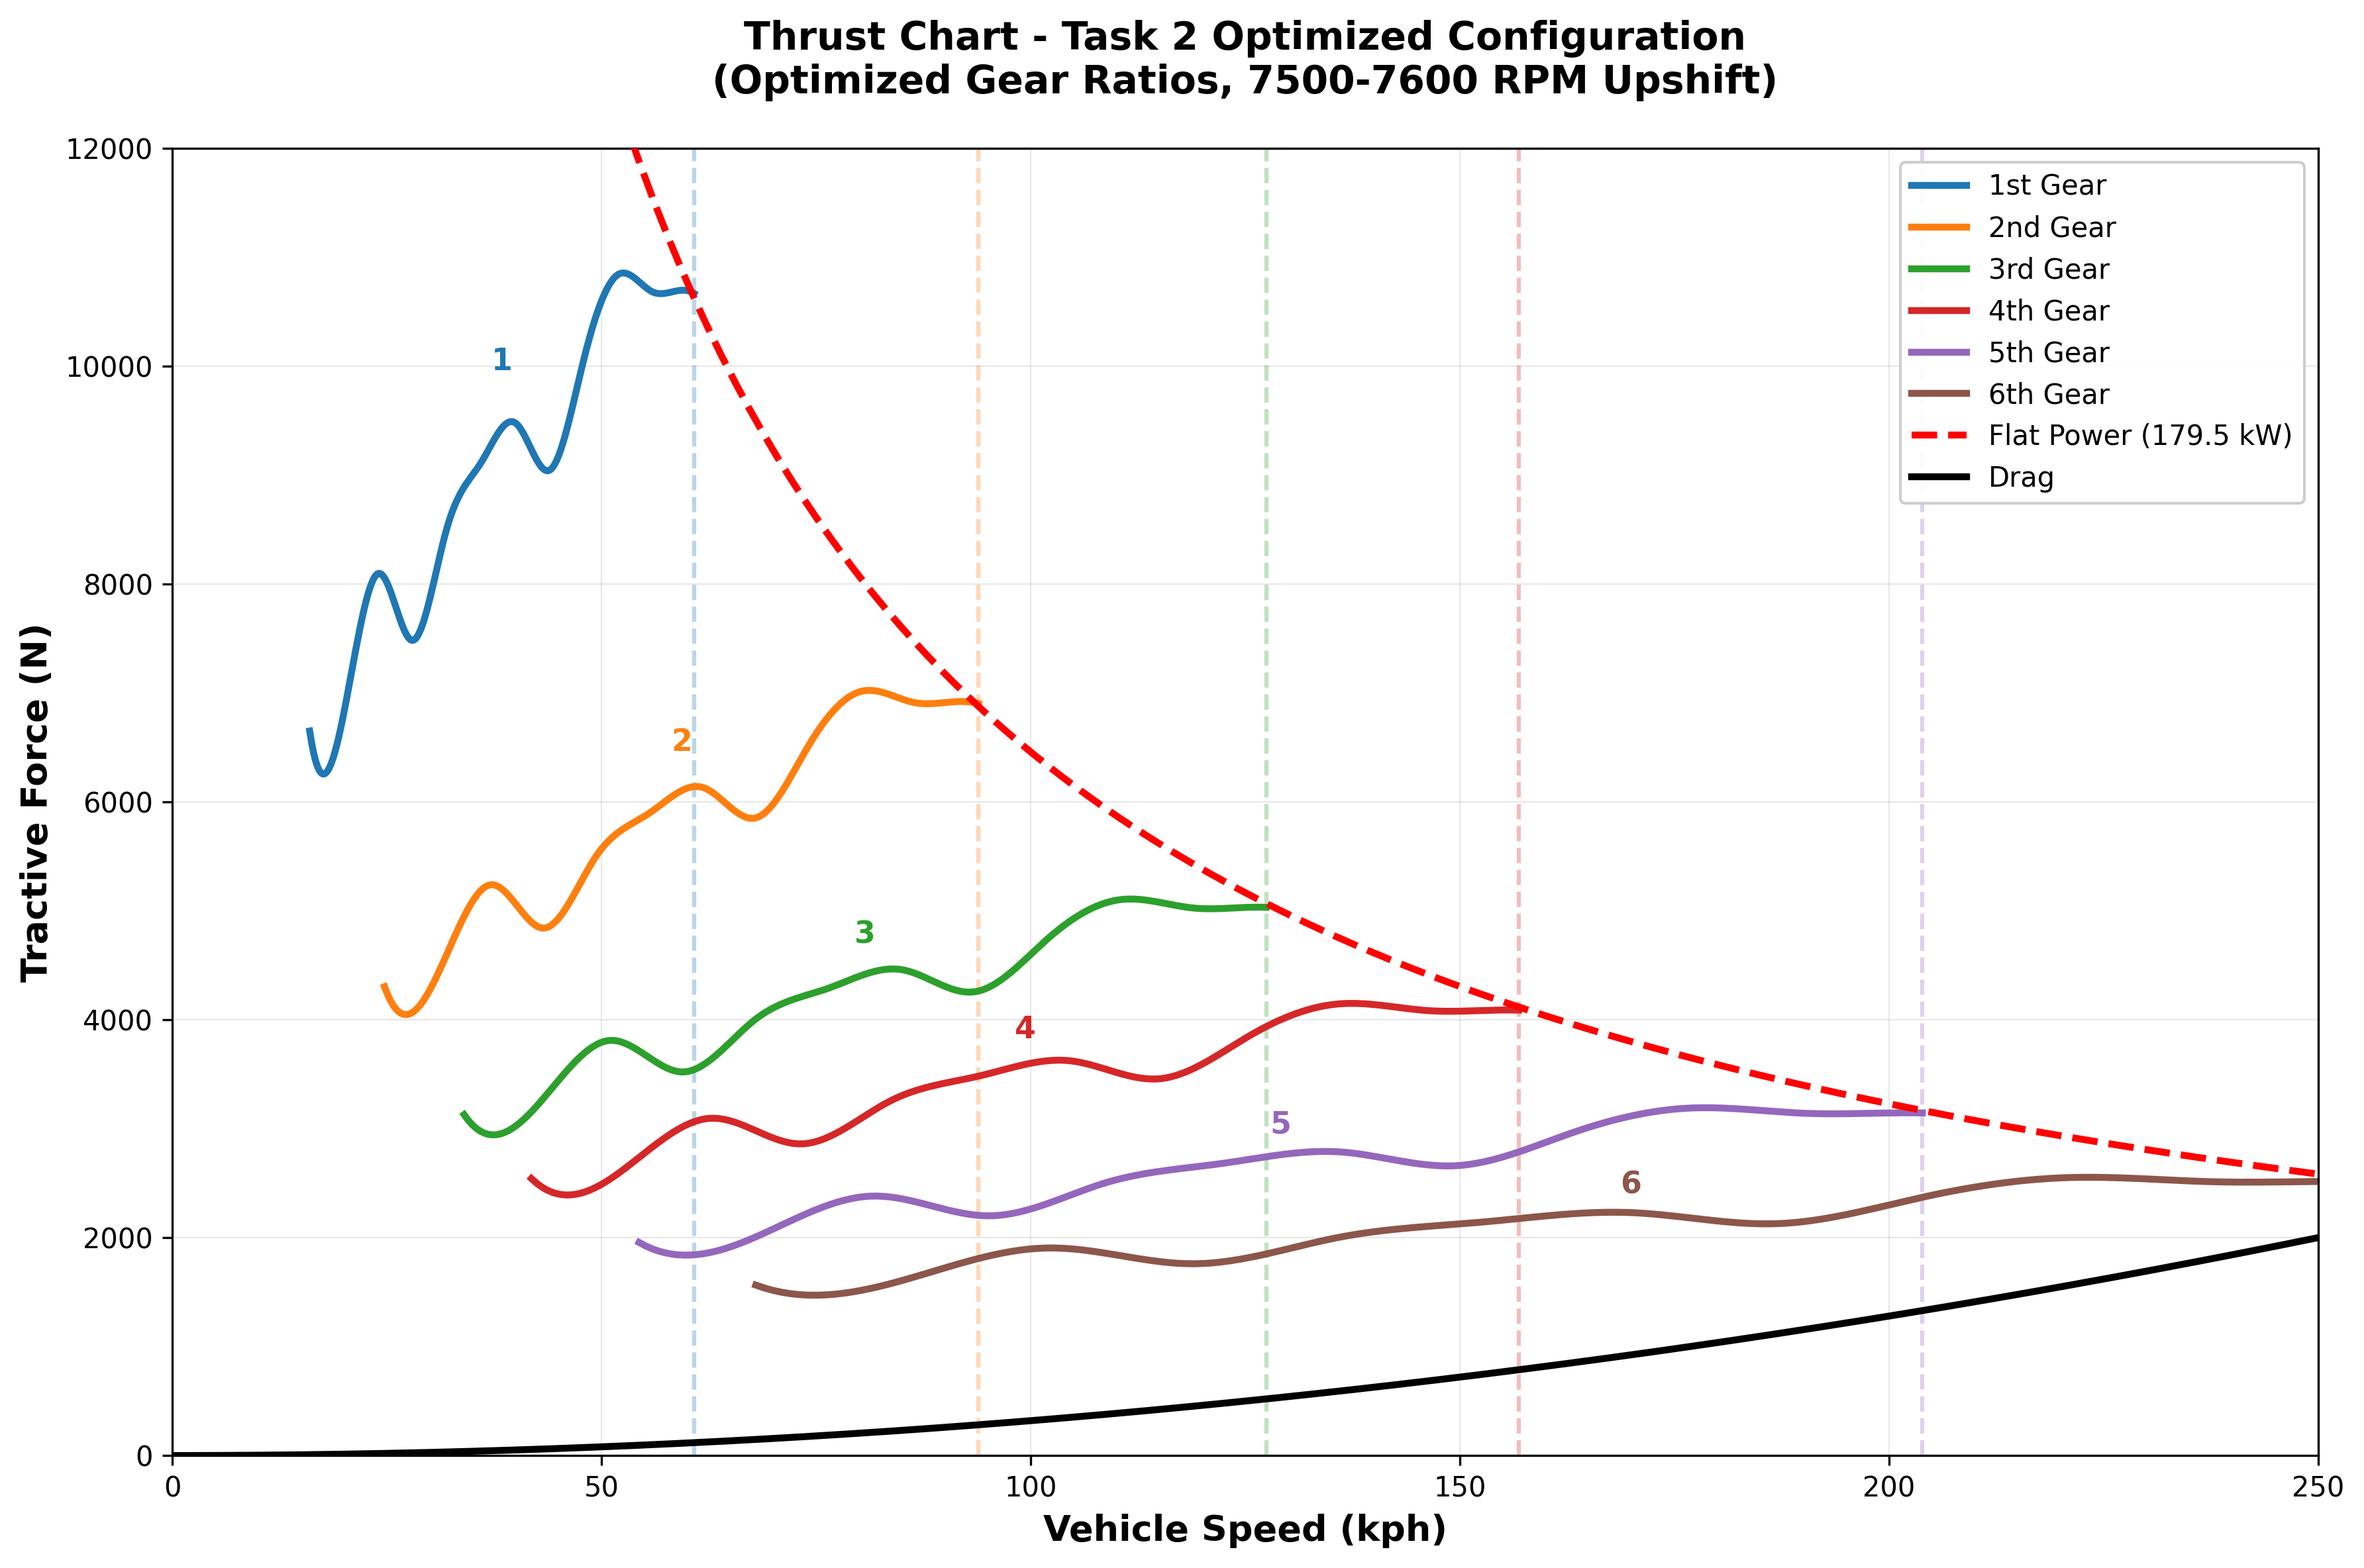
\includegraphics[width=0.75\textwidth]{task4/data/thrustcharts/thrust_chart_optimized_v2.png}
    \caption{Task 2 thrust chart (7500--7600 RPM upshift). The optimized strategy maintains engine in the high-RPM power band (6500--8000 RPM), with gear curves approaching the flat power hyperbola closely throughout the acceleration run. Flat power curve (red dashed) represents theoretical constant power delivery at 179.5 kW.}
    \label{fig:task2_thrust_optimized}
\end{figure}

\begin{figure}[H]
    \centering
    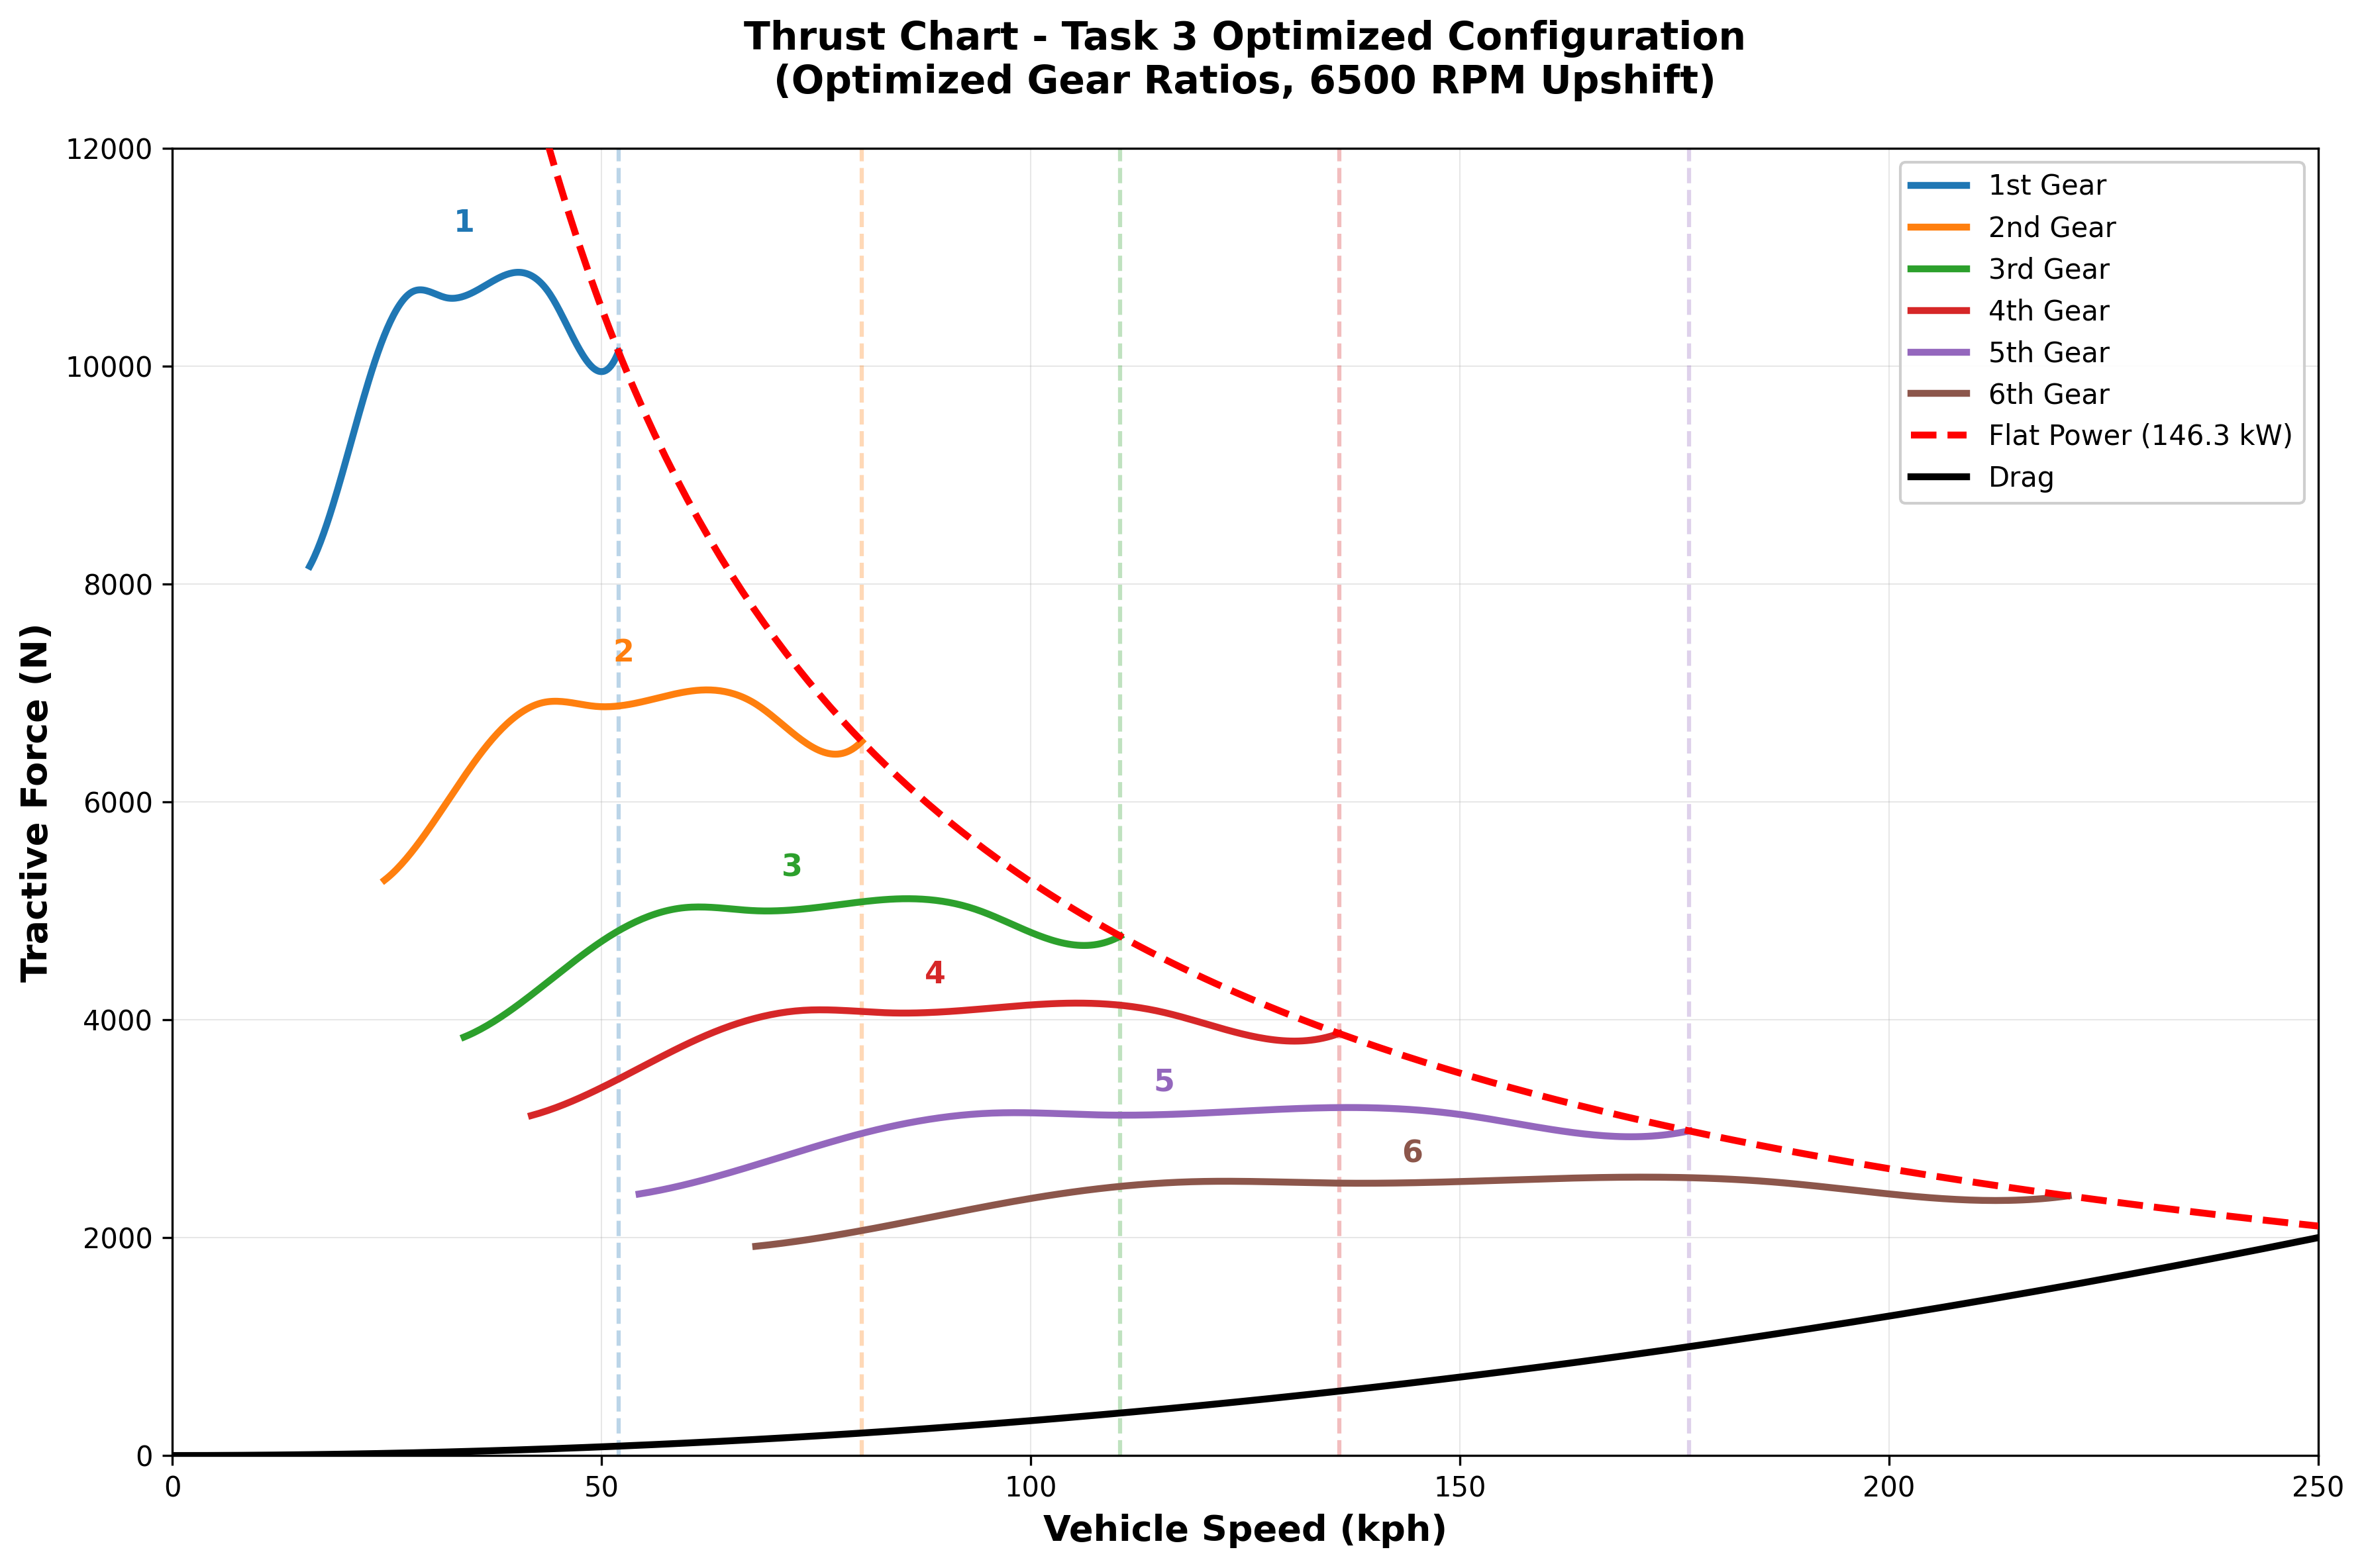
\includegraphics[width=0.75\textwidth]{task4/data/thrustcharts/thrust_chart_task3_optimized.png}
    \caption{Task 3 thrust chart (6500 RPM upshift). The optimized strategy maintains engine in the boost-developed region (3500--6500 RPM). Flatter gear curves compared to Task~2 reflect the turbocharged engine's superior low-to-mid range torque delivery, characteristic of forced induction.}
    \label{fig:task3_thrust_optimized}
\end{figure}

The thrust analysis reveals fundamental differences between the two configurations:

\begin{itemize}
    \item \textbf{Task~2:} Higher peak forces at high speeds due to superior peak power (179.5~kW vs 146.3~kW), but requires high-RPM operation for optimal performance
    \item \textbf{Task~3:} Flatter, more consistent force delivery across speed range due to broad turbo torque plateau (3500--6500~RPM)
    \item \textbf{Top speed:} Task~2 achieves ~208~kph in 6th gear, Task~3 reaches ~221~kph despite lower power, due to taller gear ratios exploiting the full 6500 RPM range
    \item \textbf{Low-speed advantage:} Task~3 delivers higher force at low speeds (below 80~kph), explaining superior 0--100~kph time (4.6s vs 5.2s)
    \item \textbf{High-speed advantage:} Task~2's higher peak power enables faster 0--160~kph time (10.3s vs 11.1s)
\end{itemize}

\subsection{Power Deployment Analysis}

\paragraph{Task~2 Power Sharing:}
The EM contribution is most significant during the 0--40~mph phase, providing up to 30\% of total system power during launch. By 80~mph, the EM contributes approximately 10--15\% of system power.

\paragraph{Task~3 Power Sharing:}
The turbocharged engine benefits from the more powerful Nissan EM61 motor. The EM provides approximately 35--40\% of system power during the 0--40~mph launch phase, significantly more than Task~2 due to the EM61's higher power capability (80~kW vs 25~kW). The EM61's contribution remains substantial at higher speeds (20--25\% of system power), helping to extend the effective power band where the turbocharged engine approaches its 6500~rpm limit.

\subsection{Weight Distribution Effects on Traction}

Weight distribution significantly affects vertical tire loads, and hence the friction limit. In this simulation, a 50/50 static weight distribution is assumed with no driver or passenger, and fuel load included. However, during dynamic launch or acceleration, weight shifts rearward, increasing the vertical load on rear tires and enhancing available traction.

If longitudinal weight transfer is considered, the rear axle may momentarily support 55--60\% of the vehicle weight. This increases $F_z$ at each driven wheel:
\begin{equation}
F_z' = \frac{0.6 \times 720 \times 9.81}{2} = 2116\, \text{N per wheel}
\end{equation}

Thus, the new friction limit becomes:
\begin{equation}
F_{x, \text{max}}' = 0.95 \cdot 2116 \approx 2010\, \text{N per wheel}
\end{equation}
\begin{equation}
T_{\text{wheel,max}}' = 2010 \cdot 0.302 \approx 607\, \text{Nm}
\end{equation}

This implies that during acceleration, the rear tires can tolerate greater wheel torque before slipping. Therefore, gear shift logic and torque maps should ideally account for transient weight transfer to utilize higher traction margins without inducing slip.

\subsection{Tire Property Effects on Simulation Results}

Tire properties play a critical role in determining vehicle performance during transient conditions, especially in acceleration tests such as the 0--100 mph simulation in Task 4. The tire behavior is modeled using the Pacejka "Magic Formula" in AVL CRUISE M, which defines the relationship between slip ratio and longitudinal force, incorporating nonlinear behavior, load sensitivity, and saturation effects.

The most influential tire parameters include:

\begin{itemize}
  \item \textbf{Friction coefficient} $(\mu)$: Determines the peak tractive force that can be generated before slip occurs.
  \item \textbf{Vertical stiffness} $(C_z)$: Affects how load is transferred between tires under acceleration, braking, or cornering.
  \item \textbf{Slip stiffness} $(C_x)$: Governs how quickly force builds up with increasing slip ratio.
  \item \textbf{Rolling radius} $(r)$: Directly influences torque transmission and effective gear ratio.
\end{itemize}

In the current simulation, tire size is set to 195/65R15, resulting in an approximate rolling radius of 0.302 m. With a rear-wheel drive layout and 50/50 static weight distribution, each rear tire supports roughly 1764 N under static conditions. During dynamic acceleration, this load increases due to longitudinal weight transfer, enhancing grip up to a point.

The implications of tire characteristics on simulation outputs are as follows:

\begin{itemize}
  \item \textbf{Acceleration Time:} A higher friction coefficient and optimized vertical load increase the peak tractive force, allowing for faster acceleration. Underestimating $\mu$ leads to premature wheel slip and torque limiting.
  \item \textbf{Wheel Slip Ratio:} Steeper slip curves result in quicker force response but may cause instability under high torque. Proper tuning ensures controlled slip in early gears.
  \item \textbf{Gear Shift Strategy:} If tires cannot transmit high torque at low gears, early upshifting may be required to avoid slipping, compromising acceleration.
  \item \textbf{Torque Limit Tuning:} Wheel torque limits are set based on tire grip; overestimation leads to unrealistic simulation results, while conservative values may underpredict performance.
\end{itemize}

Overall, accurate tire modeling ensures that the simulation reflects realistic vehicle dynamics, traction behavior, and energy efficiency. In Task 4, respecting the tire force envelope is crucial for evaluating whether engine torque and gear strategy can achieve the desired acceleration without exceeding the physical traction limits.

\subsection{Key Findings}

\begin{itemize}
    \item The Task~2 NA engine's high-RPM torque peak required aggressive shifting strategies and substantial EM compensation at low speeds, delivering strong high-speed performance
    \item The Task~3 turbocharged engine's early torque peak provided superior launch characteristics and consistent mid-range acceleration
    \item Identical gear ratios proved effective for both engines despite vastly different torque characteristics
    \item Optimized shifting strategies maintained both engines within optimal operating ranges for 70--90\% of acceleration events
    \item The P1 hybrid architecture effectively integrated with both powerplants using different electric motors: Valeo 48V (25~kW) for Task~2 and Nissan EM61 (80~kW) for Task~3
    \item Different EM power envelopes required tailored calibration strategies for each engine's torque characteristics
    \item Thrust analysis verified that gear ratio optimization successfully maintained engines in optimal RPM ranges while highlighting areas for traction-focused improvement
\end{itemize}

\subsection{Practical Implications}

\begin{itemize}
    \item \textbf{Circuit racing:} NA configuration advantageous through higher peak power
    \item \textbf{Launch performance:} Turbocharged configuration delivers superior low-to-mid speed characteristics
    \item \textbf{Both applications:} P1 hybrid architecture successfully enhances performance regardless of base ICE configuration
\end{itemize}

\subsection{Limitations and Future Work}

\subsubsection{Traction Limit Considerations}

While this study successfully optimized gear ratios for engine operating characteristics and demonstrated effective hybrid integration, several limitations warrant acknowledgment:

\paragraph{Gear Ratio Optimization Scope:}
Due to project time constraints, gear ratio optimization focused primarily on maintaining optimal engine RPM ranges (Task~2: 6500--8000~RPM, Task~3: 3500--6500~RPM) rather than explicit traction envelope matching. The thrust analysis revealed that lower gears generate tractive forces significantly exceeding theoretical tire grip limits:

\begin{itemize}
    \item 1st gear: Approximately 10,500~N peak force versus 4,238~N traction limit ($\mu = 1.2$, FWD, 360~kg front axle), representing 2.5$\times$ excess
    \item 2nd gear: Approximately 6,800~N peak force, still 1.6$\times$ above traction capacity
    \item Addition of P1 electric motor torque further compounds excess force in traction-limited scenarios, particularly during launch
\end{itemize}

\paragraph{Simulation Assumptions:}
The AVL Cruise-M transient simulations assume ideal traction management without explicit wheelspin modeling in the control strategy. Consequently:

\begin{itemize}
    \item Reported 0--100~mph times represent theoretical performance assuming perfect traction control intervention
    \item Actual acceleration times would likely be longer due to traction control limiting, wheelspin events, and driver modulation requirements
    \item Lower gear performance is optimistic, as peak forces exceed available grip by substantial margins
    \item The comparison between Task~2 and Task~3 remains valid as both configurations face similar traction limitations
\end{itemize}

\subsubsection{Recommendations for Future Development}

\paragraph{1. Traction-Optimized Gear Ratios:}
Future iterations should redesign lower gears with traction constraints as primary criteria:
\begin{itemize}
    \item 1st gear: Target ratio 2.5--2.7 (from current 3.4) to limit peak force near traction envelope ($\sim$4,500--5,000~N)
    \item 2nd gear: Target ratio 1.7--1.9 (from current 2.2) to operate closer to available grip
    \item 3rd--6th gears: Maintain current ratios as these operate in power-limited rather than traction-limited regime
\end{itemize}

This approach would improve real-world acceleration performance despite potentially longer simulated times, as traction-optimized ratios enable more effective power delivery to the road surface without excessive wheelspin.

\paragraph{2. Enhanced Traction Modeling:}
Implement dynamic traction management in simulation framework:
\begin{itemize}
    \item Tire slip ratio calculations for realistic wheelspin modeling using Pacejka Magic Formula parameters
    \item Explicit traction control system logic limiting torque to available grip based on real-time slip detection
    \item Variable friction coefficient accounting for vertical load transfer during acceleration
    \item Weight transfer effects on front axle loading for FWD configuration, particularly during high-torque launch phases
\end{itemize}

\paragraph{3. Multi-Objective Optimization Framework:}
Future gear ratio optimization should employ algorithms considering:
\begin{itemize}
    \item Traction envelope constraints as primary design criteria for gears 1--2
    \item Engine RPM optimization as primary objective for gears 3--6 (power-limited regime)
    \item Shift frequency minimization across target speed range to reduce drivetrain losses
    \item Hybrid torque blending strategies maximizing combined ICE+EM output without exceeding grip limits
    \item Launch control strategies for optimal weight transfer utilization
\end{itemize}


%========================
% REFERENCES
%========================

\begin{thebibliography}{99}

\bibitem{honda_f20c}
Wikipedia. (2025, September 5). \textit{Honda F20C engine}. \url{https://en.wikipedia.org/wiki/Honda_F20C_engine}

\bibitem{blair_racehead}
Blair, G. P. (n.d.). Designing performance - Back to basics. \textit{Racehead Engineering}. 
\url{https://racehead.com.au/designing-performance/back-to-basiscs/}

\bibitem{nascar_tech}
Baruth, J. (2010, August 5). NASCAR tech: It's a lot more than you think. \textit{The Truth About Cars}. \url{https://www.thetruthaboutcars.com/2010/08/nascar-tech-its-a-lot-more-than-you-think/}

\bibitem{bmep_comparison}
Boretti, A., Jiang, S., \& Scalzo, J. (2019). Design of direct injection jet ignition high performance naturally aspirated motorcycle engines. \textit{Designs}, \textit{3}(1), 11. \url{https://doi.org/10.3390/designs3010011}

\bibitem{honda_k20c}
Honda Motor Co. (2017). \textit{Civic Type R FK8 Technical Specifications}. Honda Engineering Documentation.

\bibitem{formula_ford}
Stone, R. (2012). \textit{Introduction to Internal Combustion Engines} (4th ed.). Palgrave Macmillan. ISBN 978-0230576636.

\bibitem{bmep_comparison}
Boretti, A., Jiang, S., \& Scalzo, J. (2019). Design of direct injection jet ignition high performance naturally aspirated motorcycle engines. \textit{Designs}, \textit{3}(1), 11. \url{https://doi.org/10.3390/designs3010011}

\bibitem{ford_ecoboost}
Ford Motor Company. (2017). \textit{1.0L EcoBoost Specification Sheet}. Ford Component Sales Technical Documentation. Retrieved from \url{https://www.ford.co.uk/content/dam/guxeu/uk/documents/home/experience-ford/about-ford/ford-component-sales/specification-details-data-sheets/10-ecoboost-np.pdf}

\bibitem{avl_cruise}
AVL List GmbH. (2024). \textit{AVL CRUISE M - Vehicle System and Driveline Simulation}. \url{https://www.avl.com/en/simulation-solutions/software-offering/simulation-tools/avl-cruise-m}

\bibitem{avl_boost}
AVL List GmbH. (2024). \textit{AVL BOOST - Engine Process Simulation}. \url{https://www.avl.com/en/simulation-solutions/software-offering/simulation-tools/avl-boost}

\bibitem{valeo_48v_motor}
Valeo. (2023). \textit{48V Electric Motor for Mild Hybrid Systems}. Valeo Powertrain Systems. \url{https://www.valeo.com/en/48v-hybridization/}

\bibitem{nissan_leaf_motor}
Wikipedia. (2025, January 15). \textit{Nissan Leaf - Electric motor}. \url{https://en.wikipedia.org/wiki/Nissan_Leaf#Powertrain}

\bibitem{nissan_em61_specs}
MarkLines Automotive Industry Portal. (2024). \textit{Nissan EM61 Motor Specifications - First Generation Leaf}. \url{https://www.marklines.com/en/vehicle/nissan/leaf}

\bibitem{ford_ecoboost}
Wikipedia. (2025, February 3). \textit{Ford EcoBoost engine}. \url{https://en.wikipedia.org/wiki/Ford_EcoBoost_engine}

\bibitem{garrett_turbo}
Garrett Motion. (2024). \textit{GT12 Series Turbochargers - Passenger Vehicle Applications}. \url{https://www.garrettmotion.com/passenger-vehicle/products/gt-series/}


\end{thebibliography}

\end{document}